% ============================================================================
% Journal of King Saud University - Computer and Information Sciences
% (Springer). Official Springer Nature LaTeX template, Basic/Name-Date
% reference style (sn-basic), matching the journal's author-year citation
% and alphabetized reference-list requirements:
% https://link.springer.com/journal/44443/submission-guidelines
% ============================================================================
\documentclass[pdflatex,sn-vancouver-num]{sn-jnl}

\usepackage[utf8]{inputenc}
\usepackage[T1]{fontenc}
\usepackage{amsmath,amssymb}
\usepackage{graphicx}
\usepackage{booktabs}
\usepackage{multirow}
\usepackage{xcolor}
\usepackage{tikz}
\usetikzlibrary{arrows.meta, positioning, fit, backgrounds, calc}
\usepackage{placeins}
\usepackage[export]{adjustbox}

\raggedbottom

% Uniform table font size across all tables in the paper, matching the
% official Springer sn-jnl template's own \tablebodyfont (8bp/9.5bp,
% class file sn-jnl.cls) rather than an ad hoc size. Applied via
% \adjustbox{max width=\textwidth}{...}, which shrinks a table further only
% if it would still overflow \textwidth at this size, and never enlarges a
% narrower table -- unlike \resizebox{\textwidth}{!}, which forced every
% table to fill the full width and made font size vary table to table
% depending on content. tableorg bypasses the class's own table environment
% (used to avoid a threeparttable/resizebox interaction bug), so
% \tablebodyfont is not applied automatically and must be invoked explicitly.
\newcommand{\uniformtablesize}{\tablebodyfont}

% Per-appendix table numbering (Table A1, A2, ...; Table B1, ...; etc.)
\newcommand{\appendixtablenumbering}[1]{%
  \renewcommand{\thetable}{#1\arabic{table}}%
  \renewcommand{\theHtable}{appendix-#1.\arabic{table}}%
  \setcounter{table}{0}%
}

% ============================================================================
% BLINDED MANUSCRIPT for double-blind review (Journal of King Saud University
% - Computer and Information Sciences). Author names, affiliations, and
% contact information are intentionally omitted here and submitted separately
% via titlepage.tex, per the journal's double-blind review policy:
% https://link.springer.com/journal/44443/submission-guidelines
% ============================================================================

\begin{document}

\title{Improving Lightweight Super-Resolution via Depth Compression: A Statistically-Validated Accuracy--Efficiency Trade-off for Ear Biometrics}

\abstract{Ear recognition is gaining attention as a complement to face recognition, but ear images are often captured well below the resolution lightweight super-resolution (SR) architectures such as SPAN were designed for. This paper asks how far such a model can be compressed before it stops helping, and how much of the resulting gap SR closes, answering both with span\_tiny, a depth-compressed SPAN variant (3 attention blocks instead of 6, a 46.0\% parameter reduction) evaluated across eleven backbones with multi-seed testing. On the primary dataset (EarVN1.0), span\_tiny and the uncompressed baseline both significantly improve identity accuracy over no-SR in nearly every backbone; the accuracy cost of compression reaches significance in only one of eleven backbones and is negligible overall (equivalence test, $p=0.008$). A frequency-domain test explains why: removing the lowest 10\% of the spectrum collapses accuracy to near chance in all eleven backbones, while keeping only that band preserves a quarter of it, so identity-relevant signal survives compression because it lives in coarse, low-frequency structure. Against a high-resolution ceiling, SR recovers only a fifth to a quarter of the gap, matched almost exactly by the uncompressed baseline. The compression-safety finding replicates on a second dataset, AWEx (336 subjects, three protocols, zero of eleven backbones showing a cost), and against five other lightweight SR architectures span\_tiny is never beaten, tying the top performers at a fraction of their parameter count. One exception: on low-resolution images, one backbone (ResNet-18) reverses this ordering, traced to a train/test resolution mismatch.}

\keywords{lightweight super-resolution, depth compression, ear recognition, low-resolution biometrics, equivalence testing}

\maketitle

% ============================================================================
\section{Introduction}
% ============================================================================

\subsection{Background}

Ear biometrics has drawn growing interest as a complement or alternative to face recognition, particularly since widespread mask-wearing made face-based identification unreliable in many settings~\cite{mehta2023ear}. The ear offers several properties useful for identification: its structure remains largely stable across adulthood, it carries a distinctive pattern of cartilage folds, and it changes little with facial expression, unlike the face. However, ear recognition in unconstrained settings (surveillance footage, images captured at a distance) routinely produces ear regions at very low pixel resolution, often well below what recognition backbones or SR networks were designed for.

Deep-learning-based SR began with Dong et al.'s SRCNN~\cite{dong2016srcnn}, a shallow end-to-end CNN mapping directly from LR to HR pixels, and was made computationally practical at higher resolutions by Shi et al.'s sub-pixel convolution~\cite{shi2016espcn}, which moved upsampling to the final layer via a learned pixel-shuffle operation, the same upsampling mechanism SPAN itself uses (Section~\ref{sec:arch}). A separate branch pursued perceptual realism over pixel fidelity: Ledig et al.'s SRGAN~\cite{ledig2017srgan} combined an adversarial loss with a perceptual feature loss to produce photo-realistic detail at high upscaling factors, an objective distinct from the pixel- and distillation-based training recipe used in this paper (Section~\ref{sec:recipe}), where the downstream task rather than perceptual quality is the target. Lightweight SR has advanced considerably since, driven largely by the NTIRE efficient super-resolution challenge series. SPAN~\cite{wan2024span} is among the most efficient recent designs. It won both the overall-performance and runtime tracks of NTIRE 2024 by replacing learned attention (of the kind popularized for vision by squeeze-and-excitation channel gating~\cite{hu2018senet}) with a symmetric, parameter-free activation applied directly to convolutional outputs. Other designs pursue efficiency through different mechanisms: RLFN~\cite{kong2022rlfn} simplifies feature aggregation, ECBSR~\cite{zhang2021ecbsr} uses hardware-friendly re-parameterized convolutions in the same general spirit as RepVGG's structural re-parameterization for classification backbones~\cite{ding2021repvgg}, SAFMN~\cite{sun2023safmn} relies on spatially-adaptive modulation instead of self-attention, and SMFANet~\cite{zheng2024smfanet} combines self-modulation with a lightweight feed-forward design. All of these architectures are designed and benchmarked at input resolutions of roughly 32--64\,px or higher, well above the $\sim$20$\times$20-pixel regime addressed in this paper, and none has been evaluated for further depth compression under statistically rigorous validation against a concrete downstream task.

\subsection{Research gap}

Two gaps motivate this work. First, most lightweight SR papers report PSNR and SSIM on standard benchmarks such as Set5, Set14, Urban100, and DIV2K. These metrics say little about whether a compressed model remains useful as a pre-processing step for a specific recognition task at extremely low input resolution. Some precedent exists for optimizing SR toward a downstream task rather than pixel fidelity: Ataer-Cansizoglu et al.~\cite{ataer2019identity} demonstrated this for low-resolution face verification. Almost no equivalent work exists for ear biometrics, and none addresses how far a lightweight architecture can be compressed before downstream accuracy degrades. Second, papers in this area typically report a single training run without a variance estimate, making it difficult to determine whether a reported accuracy gap reflects a genuine effect or seed-to-seed noise. This concern is more acute for downstream classification accuracy than for SR pixel metrics, since classification accuracy is a noisier signal, and a single run therefore provides weaker support for a claim than it would for PSNR.

\subsection{Contributions}

This paper's central contribution is span\_tiny, a depth-compressed variant of SPAN (\texttt{n\_blocks} reduced from 6 to 3) that cuts parameter count by 46.0\% and measured inference latency by 54.8\% (Table~\ref{tab:quality}; not a deployment benchmark, Section~\ref{sec:limitations}); the re-implementation matches 99.93\% of the original authors' published SPAN-S benchmark PSNR. Four results carry most of the paper's evidentiary weight. First, multi-seed ($n=5$), multi-backbone (eleven recognition architectures) testing shows both span\_tiny and the uncompressed baseline beat no-SR significantly in all eleven backbones on EarVN1.0, while the accuracy cost of compression itself reaches significance in only one, a finding that replicates on a second, independent dataset (AWEx, 336 subjects) across three evaluation protocols, with no backbone showing a significant cost under any of them. Second, a depth ablation isolating block count alone (span\_tiny vs.\ span\_large, an otherwise identical, uncompressed-depth counterpart) shows no significant difference in ten of eleven backbones on EarVN1.0 and all eleven on AWEx, the methodologically cleanest test of the central claim. Third, span\_tiny is never significantly beaten on downstream accuracy by five other lightweight SR architectures (RLFN, RLFN-adapted, ECBSR, SAFMN, SMFANet) trained under an identical distillation recipe, despite ranking low among them on raw PSNR/SSIM. Fourth, a direct frequency-domain ablation (Section~\ref{sec:freq-ablation}) answers not whether compression is safe but why: filtering span\_tiny's SR output and re-evaluating each backbone's already-trained recognition model, no retraining, shows removing the lowest 10\% of the spectrum collapses accuracy to 2.9--5.1\% of baseline, while retaining only that band preserves 22.3--33.6\% of it, with zero exceptions across all eleven backbones: direct, cross-backbone evidence that the recognition-relevant signal in a low-resolution ear crop is concentrated in coarse, low-frequency structure a shallow network already captures.

Several secondary results round out the picture without carrying the same weight: a loss-component ablation finds the identity term significantly reduces downstream accuracy (consistent with an independent hyperparameter sweep, Section~\ref{sec:recipe}) while the distillation term's own contribution is statistically indistinguishable from pixel-only training; three further mechanisms designed to improve on span\_tiny beyond its core block-count reduction (feature-level distillation, a saliency-weighted loss, learned/differentiable block pruning) each fail to help, with learned pruning performing significantly worse than the fixed block selection it replaces in nearly every backbone; and an ablation testing this paper's own initial candidate explanation for depth tolerance (that SPAN's attention mechanism carries no learned parameters) finds no support for it across 22 backbone--architecture combinations, which motivated the direct frequency-domain test above rather than leaving that account untested.

To support reproducibility, the complete source code, pipeline scripts, and a step-by-step reproduction guide are publicly available at \url{https://github.com/quangthai121121/earsr_span}.

\subsection{Paper organization}

The remainder of this paper is organized as follows. Section~\ref{sec:related} reviews related work on ear recognition, efficient super-resolution, SR for downstream recognition, and knowledge distillation. Section~\ref{sec:method} presents span\_tiny's architecture, the distillation recipe, and the statistical methodology used throughout. Section~\ref{sec:setup} details the experimental setup across both datasets. Section~\ref{sec:results} reports the main and contextual results, the negative-result ablations of Section~\ref{sec:novelty-ablations}, and the extended mechanism ablations of Section~\ref{sec:extended-ablations}. Section~\ref{sec:discussion} discusses mechanism and scope, Section~\ref{sec:limitations} states limitations, and Section~\ref{sec:conclusion} concludes.

% ============================================================================
\section{Related Work}
\label{sec:related}
% ============================================================================

\subsection{Ear recognition}

Ear recognition moved from handcrafted descriptors toward deep-learning approaches over the past decade, with the earliest CNN-based work already flagging a constraint that still shapes experimental design in this area: Alshazly et al.~\cite{alshazly2020unconstrained} trained an ensemble of CNNs for unconstrained ear recognition and found data augmentation and transfer learning essential given the small size of available ear datasets, including the dataset choices made in this paper (Section~\ref{sec:datasets}). A second line of work targets efficient, edge-deployable recognition, paralleling the push toward efficient SR discussed next (Section~\ref{sec:related-sr}): Mehta and Singh~\cite{mehta2023ear} developed a lightweight CNN for 2D ear recognition motivated by widespread mask-wearing making face-based identification unreliable, targeting CPU-only embedded hardware, and Lendering et al.~\cite{lendering2025edgeear} proposed EdgeEar, a hybrid CNN--transformer with low-rank linear layers that cuts parameter count by roughly 50$\times$ relative to prior state-of-the-art ear recognition models while achieving the lowest equal-error rate on the UERC2023 benchmark~\cite{emersic2023uerc}. A third, more recent line pushes accuracy and robustness directly: Peddi et al.~\cite{peddi2025proton} report rank-1 accuracy above 99\% with a prototype-node graph neural network for multi-impression ear recognition; Arun et al.~\cite{arun2025vitear} show that overlapping-patch tokenization substantially improves Vision Transformer ear verification, including on EarVN1.0; Ozturk et al.~\cite{ozturk2025bilateral} demonstrate that treating left and right ears as distinct classes during training improves CNN-based ear recognition, direct evidence for the left-right asymmetry this paper also relies on in choosing not to apply horizontal-flip augmentation (Section~\ref{sec:impl}); and Mohamed et al.~\cite{mohamed2024earbiometrics} report near-ceiling accuracy on EarVN1.0 itself under full-resolution, unconstrained-augmentation training, a regime very different from the extreme $20\times20$-pixel setting studied here (Section~\ref{sec:results}). Benzaoui et al.~\cite{benzaoui2023survey} provide a broader survey spanning 2D, 3D, and hybrid ear recognition approaches, databases, and open challenges.

Publicly available ear datasets vary substantially in scale, acquisition conditions, and subject count. EarVN1.0~\cite{hoang2019earvn} is a large-scale, in-the-wild dataset of 28{,}412 color images from 164 Vietnamese subjects (98 male, 66 female), collected under unconstrained illumination and pose. The Annotated Web Ears (AWE) dataset~\cite{emersic2017ear} and its extensions (collectively AWEx in this work) were assembled by the University of Ljubljana ear-recognition research group, the same group behind EdgeEar~\cite{lendering2025edgeear}, from web-crawled images of public figures. The base AWE set contains 1{,}000 images from 100 subjects. This paper extends it with the CVL Ear dataset (16 subjects, 804 images) and an additional ``New Images'' collection (220 subjects, 2{,}200 images) from the same research group, giving a combined pool of 336 subjects and 4{,}004 images (Section~\ref{sec:datasets}).

\subsection{Lightweight/efficient super-resolution}
\label{sec:related-sr}

Recent efficient SR research has been substantially driven by the NTIRE efficient super-resolution challenge series. RLFN~\cite{kong2022rlfn} simplifies feature aggregation to three convolutional layers per residual block, winning the runtime track of NTIRE 2022. ECBSR~\cite{zhang2021ecbsr} proposes edge-oriented convolution blocks that re-parameterize multiple operations into a single 3$\times$3 convolution at inference time, targeting real-time performance on commodity mobile SoCs. SAFMN~\cite{sun2023safmn} introduces a spatially-adaptive feature modulation mechanism that captures non-local dependencies without the computational cost of dot-product self-attention, achieving parameter counts roughly 3$\times$ smaller than IMDN at comparable quality. SMFANet~\cite{zheng2024smfanet} combines a self-modulation feature aggregation module with a partial-convolution feed-forward network to balance local and non-local feature interaction efficiently. SPAN~\cite{wan2024span}, the architecture compressed in this work, replaces learned attention with a parameter-free mechanism based on symmetric activation functions applied to convolutional outputs, winning both the overall-performance and runtime tracks of NTIRE 2024~\cite{ren2024ntire}. The challenge itself has continued past SPAN's 2024 edition, with the 2025 edition~\cite{ren2025ntire} reporting incremental gains from newer entrants rather than a change in the field's overall efficiency frontier. Several further lightweight designs have appeared since SPAN, exploring complementary directions: involution combined with blueprint-separable convolutions~\cite{khatami2025ibmdn}, hybrid channel/spatial attention under a fully separable-convolution backbone~\cite{cao2024hasn}, Mamba-based state-space blocks compressed via low-rank knowledge distillation for edge deployment~\cite{aalishah2025mambalitesr}, and lightweight transformers trained without access to genuine high-resolution supervision~\cite{moller2025lronly}. All of these, like the architectures above, target standard SR benchmarks at input resolutions well above the regime studied here, and none has been evaluated for depth compression below its original design point under a downstream recognition objective at extremely low input resolution ($\approx$20$\times$20\,px).

\subsection{Super-resolution for downstream recognition}

Recognition accuracy on low-resolution imagery does not follow directly from pixel-fidelity metrics. Wang et al.~\cite{wang2016vlrr} showed this directly for very-low-resolution recognition (face identification, digit recognition, and font recognition), finding that networks trained and evaluated with resolution-appropriate objectives outperform those optimized for a fixed higher resolution. A separate line of work optimizes SR explicitly for downstream recognition accuracy instead of pixel fidelity. Ataer-Cansizoglu et al.~\cite{ataer2019identity} trained an identity-preserving face SR network to minimize distance in a pre-trained face-recognition feature space instead of pixel space, and found that this recognition-aware objective outperformed conventional pixel-fidelity SR for very-low-resolution face verification. The same question has been asked for iris biometrics. Nguyen et al.~\cite{nguyen2011iris} showed that SR tailored for recognition at a distance improves iris matching more than generic SR does. Ribeiro et al.~\cite{ribeiro2019iris} asked directly whether photo-realistic reconstruction is necessary for iris recognition, and found that the two are related but not the same objective, matching the finding Ataer-Cansizoglu et al.\ report for faces. The qualitative results in this paper echo the same pattern (Figure~\ref{fig:qualitative}b, Section~\ref{sec:res-main}): a near-tied, relatively high PSNR turns out to be driven by accurate reconstruction of hair and background rather than of the ear itself. Ear biometrics has not yet been examined through this lens. The evaluation of span\_tiny directly on downstream identity accuracy, rather than on PSNR/SSIM alone, extends the same question to a modality where it has not previously been asked.

\subsection{Knowledge distillation in super-resolution}

Teacher--student distillation~\cite{hinton2015distilling} is a common strategy for training compact SR networks, typically combining a pixel-reconstruction loss with a feature- or output-level distillation loss against a larger teacher network. The idea of supervising a compact student's intermediate representations directly, rather than only its final output, traces to Romero et al.'s FitNets~\cite{romero2015fitnets}; the feature-level distillation term evaluated as ``KD v2'' in this paper's own negative-result ablation (Section~\ref{sec:novelty-ablations}) is a direct descendant of this idea, applied at the SR feature level instead of a classification backbone's. Lee et al.~\cite{lee2020privileged} distilled intermediate decoder features from a teacher trained with privileged access to the HR image, letting the student recover high-frequency detail it could not learn from LR input alone. Zhang et al.~\cite{zhang2024dukd} argued that a core assumption behind most SR distillation methods does not hold: because a teacher's own SR output is itself only a noisy approximation of the true HR image, naively matching student outputs to teacher outputs caps how much the student can improve. Their proposed data-upcycling scheme was designed specifically to work around this ceiling. Jiang et al.~\cite{jiang2024mtkd} instead pool supervision from multiple teacher SR networks simultaneously via a feature-alignment strategy that reconciles their differing representations, an orthogonal direction to the single-teacher recipe used in this paper; for a broader treatment of distillation mechanisms across modalities, see the recent survey by Mansourian et al.~\cite{mansourian2025kdsurvey}. This observation offers a useful lens on the findings reported here: the loss-ablation in Section~\ref{sec:res-loss} finds no statistically significant contribution of the distillation term to downstream accuracy at this compression level, which is consistent with distillation gains for SR being real but small and hard to detect against a noisy teacher signal, rather than with distillation being useless. The recipe used in this paper (Section~\ref{sec:recipe}) is simpler than either of these, and this paper additionally reports a rigorous ablation of its contribution to \emph{downstream recognition accuracy} specifically, a question this literature has not directly addressed.

\subsection{Positioning}

To our knowledge, no prior work combines further depth compression of a state-of-the-art parameter-free-attention SR architecture, evaluation at an extremely low input resolution (20$\times$20\,px) substantially below the design regime of the compared architectures, and multi-seed, multi-backbone statistical validation against a downstream ear-recognition task, confirmed across two independent datasets. This combination of experimental conditions is not itself the contribution: what it enables is a testable account of \emph{why} depth compression is tolerable here at all: that the recognition-relevant signal in a low-resolution ear crop is concentrated in coarse, low-frequency structure a shallower network already captures, a candidate explanation tested directly, both against two architectures with learned (rather than parameter-free) attention and via direct frequency-domain ablation of what a trained recognition model's own predictions depend on, rather than assumed (Section~\ref{sec:disc-depth}). This paper addresses both the experimental combination and this candidate mechanistic account.

% ============================================================================
\section{Methodology}
\label{sec:method}
% ============================================================================

\subsection{Problem formulation}

Given a high-resolution ear crop, a low-resolution counterpart is generated via bicubic downsampling at a fixed scale factor $\times4$ (HR 80$\times$80 $\to$ LR 20$\times$20 on EarVN1.0; HR 76$\times$76 $\to$ LR 19$\times$19 on AWEx, since \texttt{hr\_size} is auto-selected per dataset, Section~\ref{sec:datasets}). An SR model upsamples the LR image back to the dataset's HR size, and the resulting image is passed to a recognition backbone trained to predict subject identity and, secondarily, gender. Three domains are compared throughout: \texttt{lr} (no SR, the LR image bicubically upsampled and fed directly to the recognition backbone, establishing the no-SR baseline), \texttt{span\_baseline} (the uncompressed SPAN architecture, referred to as \texttt{sr\_baseline} in project logs), and \texttt{span\_tiny} (the depth-compressed variant proposed here, referred to as \texttt{sr\_improved}).

The SPAN-family names used throughout this paper are collected in Table~\ref{tab:terminology} for reference, since the same underlying architecture is instantiated in several configurations that differ only in block count or in which of the two implementations (custom re-implementation vs.\ original authors' code) is used, and these are each introduced separately across this and later sections.

\begin{tableorg}[htbp]
\centering
\caption{SPAN-family terminology used throughout this paper. All configurations share the same overall architecture (Figure~\ref{fig:arch}); they differ only in block count (\texttt{n\_blocks}) and in which of two implementations is used (Section~\ref{sec:arch}).}
\label{tab:terminology}
\adjustbox{max width=\textwidth}{\uniformtablesize%
\begin{tabular}{lll}
\toprule
Paper name & Blocks / implementation & Role \\
\midrule
\texttt{span\_tiny} & 3 blocks, custom re-implementation & This paper's proposed, depth-compressed model \\
\texttt{span\_baseline} & 6 blocks, original authors' code & Uncompressed reference in the main comparison (Table~\ref{tab:main}) \\
\texttt{span\_large} & 6 blocks, custom re-implementation & Uncompressed counterpart isolating depth alone (Table~\ref{tab:depth}) \\
\texttt{lr} & -- (no SR) & Bicubic-upsampled input, no-SR baseline \\
\bottomrule
\end{tabular}
}
\end{tableorg}

\subsection{span\_tiny architecture}
\label{sec:arch}

span\_tiny is a depth-compressed variant of SPAN~\cite{wan2024span}. Where the uncompressed baseline uses \texttt{n\_blocks=6} Swift Parameter-free Attention Blocks (SPABs) at \texttt{feat=48} channels, span\_tiny uses \texttt{n\_blocks=3} at the same channel width, reducing deploy-mode parameters from 0.4263M to 0.230M ($-46.0\%$). Each SPAB (Figure~\ref{fig:arch}a) passes its input $x$ through three sequential 3$\times$3 convolutions, the first two followed by GELU, to obtain raw features $h$. These raw features feed two parallel, independently-computed paths: a residual sum $u = x + h$, and a parameter-free attention map $v = \mathrm{sigmoid}(h) - 0.5$, a fixed activation symmetric about the origin with no learned parameters. The block output is formed by element-wise multiplication applied last, $\text{output} = u \otimes v$: the residual is added before, not after, the attention modulation. Each SPAN stack additionally carries a block-level global residual, in which the feature map immediately after the initial shallow feature-extraction convolution is added back after the final feature-aggregation convolution, immediately before pixel-shuffle upsampling (Figure~\ref{fig:arch}b,c). Halving the number of SPABs removes attention \emph{computation} across the removed blocks but not attention \emph{parameters}, since the mechanism has none. This property is proposed in Section~\ref{sec:disc-depth} as a partial explanation for why the ablation in Section~\ref{sec:res-depth} shows minimal accuracy degradation from depth reduction.

Before applying span\_tiny to the ear-recognition task, the re-implementation was validated against the original authors' published results. On the SPAN-S benchmark configuration reported in~\cite{wan2024span} (Table~1), the re-implementation reproduces 99.93\% of the reported PSNR, indicating that observed differences in the ear-recognition experiments reflect the compression itself rather than an implementation discrepancy.

span\_tiny and span\_large (the uncompressed-depth counterpart used in the depth ablation, Section~\ref{sec:res-depth}) are both instantiated from the same custom \texttt{SPAN} class shown in Figure~\ref{fig:arch}a, using plain 3$\times$3 convolutions and differing only in \texttt{n\_blocks} (3 vs.\ 6). This makes the span\_tiny-vs-span\_large comparison (Table~\ref{tab:depth}) a clean, single-variable isolation of depth. By contrast, \texttt{span\_baseline} (used in Table~\ref{tab:main} as the uncompressed reference and referred to as \texttt{span\_official} in project logs) is instantiated from the original authors' SPAN codebase, which internally uses a reparameterizable Conv3XC convolution design, in the same structural-reparameterization spirit as RepVGG~\cite{ding2021repvgg}, rather than plain 3$\times$3 convolutions. Both implementations are architecturally equivalent at deploy time, since Conv3XC collapses to an equivalent single convolution after re-parameterization, and both are validated against the same published SPAN-S benchmark numbers, but they are not byte-for-byte the same low-level implementation. This is the source of the small parameter-count difference between span\_large (0.417M, plain-conv 6-block) and span\_baseline (0.4263M, Conv3XC-based 6-block) visible in Table~\ref{tab:quality}, despite both being nominally 6-block, 48-channel configurations. Table~\ref{tab:depth} (span\_tiny vs.\ span\_large) is therefore treated as the methodologically cleaner test of the depth-compression hypothesis, while Table~\ref{tab:main} (span\_tiny vs.\ span\_baseline) answers the closely related but distinct practical question of how the compressed model compares against deploying the official pre-trained baseline. This distinction is made explicit here so that neither table is over-interpreted as isolating a variable it does not fully isolate.

% ---------------------------------------------------------------------------
\begin{figure}[htbp]
\centering
\adjustbox{max width=\textwidth}{\uniformtablesize%
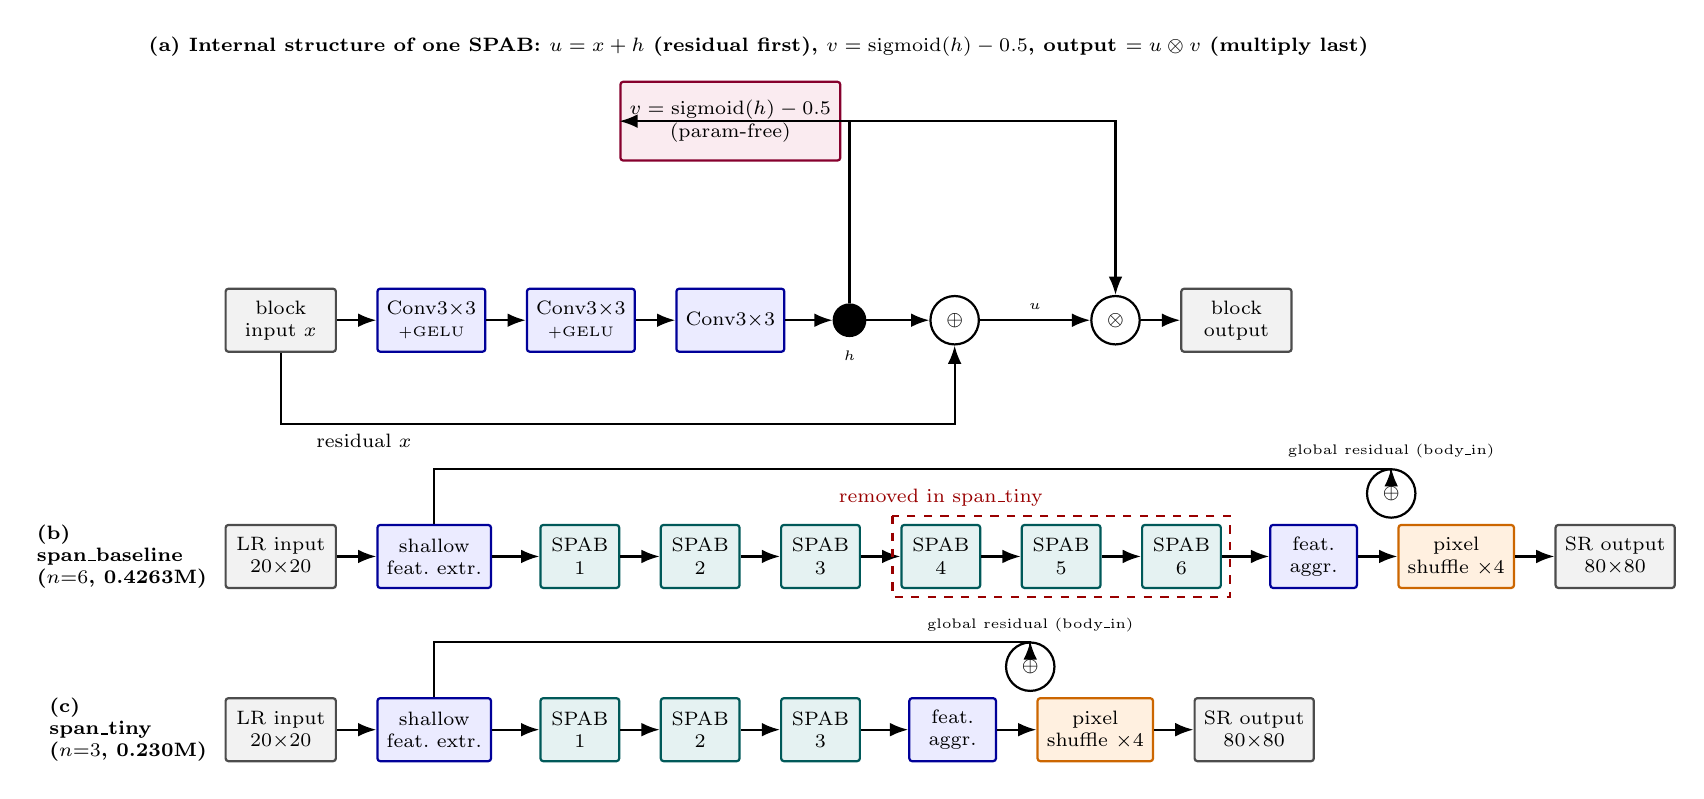
\begin{tikzpicture}[
  font=\scriptsize,
  >=Latex,
  node distance=5mm,
  io/.style       ={rectangle, draw=black!70, thick, rounded corners=1pt, minimum height=8mm, minimum width=14mm, align=center, fill=black!5},
  conv/.style     ={rectangle, draw=blue!60!black, thick, rounded corners=1pt, minimum height=8mm, minimum width=11mm, align=center, fill=blue!8},
  spab/.style     ={rectangle, draw=teal!70!black, thick, rounded corners=1pt, minimum height=8mm, minimum width=10mm, align=center, fill=teal!10},
  up/.style       ={rectangle, draw=orange!80!black, thick, rounded corners=1pt, minimum height=8mm, minimum width=14mm, align=center, fill=orange!12},
  arr/.style      ={->, thick},
]

% ---------- Panel (a): internal SPAB block structure ----------
\begin{scope}[local bounding box=inset]
\node[io] (bin) {block\\input $x$};
\node[conv, right=of bin] (c1) {Conv3$\times$3\\{\tiny+GELU}};
\node[conv, right=of c1] (c2) {Conv3$\times$3\\{\tiny+GELU}};
\node[conv, right=of c2] (c3) {Conv3$\times$3};
\node[circle, draw=black, thick, minimum size=4mm, right=6mm of c3, fill=black] (hpt) {};
\node[below=0.5mm of hpt, font=\tiny] {$h$};

\node[rectangle, draw=purple!70!black, thick, rounded corners=1pt, minimum height=10mm, minimum width=22mm, fill=purple!8, align=center, above=16mm of c3] (sig) {$v=\mathrm{sigmoid}(h)-0.5$\\\scriptsize(param-free)};
\node[circle, draw=black, thick, minimum size=5mm, right=8mm of hpt] (add) {$\oplus$};
\node[circle, draw=black, thick, minimum size=5mm, right=14mm of add] (mult) {$\otimes$};
\node[io, right=of mult] (bout) {block\\output};

\draw[arr] (bin) -- (c1);
\draw[arr] (c1) -- (c2);
\draw[arr] (c2) -- (c3);
\draw[arr] (c3) -- (hpt);
\draw[arr] (hpt) -- (add);
\draw[arr] (hpt.north) |- (sig.west);
\draw[arr] (sig.east) -| (mult.north);
\draw[arr] (add) -- node[above,font=\tiny]{$u$} (mult);
\draw[arr] (bin.south) -- ++(0,-9mm) -| node[pos=0.05,below,xshift=2mm]{residual $x$} (add.south);
\draw[arr] (mult) -- (bout);
\end{scope}

\node[above=2mm of inset, font=\bfseries\scriptsize] {(a) Internal structure of one SPAB: $u=x+h$ (residual first), $v=\mathrm{sigmoid}(h)-0.5$, output $=u\otimes v$ (multiply last)};

% ---------- Panel (b): span_baseline (n_blocks=6) ----------
\begin{scope}[yshift=-30mm]
\node[io] (lr) {LR input\\20$\times$20};
\node[conv, right=of lr] (sfe) {shallow\\feat.\ extr.};
\node[spab, right=6mm of sfe] (b1) {SPAB\\1};
\node[spab, right=of b1] (b2) {SPAB\\2};
\node[spab, right=of b2] (b3) {SPAB\\3};
\node[spab, right=of b3] (b4) {SPAB\\4};
\node[spab, right=of b4] (b5) {SPAB\\5};
\node[spab, right=of b5] (b6) {SPAB\\6};
\node[conv, right=6mm of b6] (agg) {feat.\\aggr.};
\node[up, right=of agg] (ps) {pixel\\shuffle $\times$4};
\node[io, right=of ps] (sr) {SR output\\80$\times$80};

\draw[arr] (lr)--(sfe); \draw[arr] (sfe)--(b1); \draw[arr] (b1)--(b2); \draw[arr] (b2)--(b3);
\draw[arr] (b3)--(b4); \draw[arr] (b4)--(b5); \draw[arr] (b5)--(b6); \draw[arr] (b6)--(agg);
\draw[arr] (agg)--(ps); \draw[arr] (ps)--(sr);
\node[circle, draw=black, thick, minimum size=4mm, right=1mm of agg, yshift=8mm] (gadd) {$\oplus$};
\draw[arr] (sfe.north) -- ++(0,7mm) -| node[pos=0.5,above,font=\tiny]{global residual (body\_in)} (gadd.north);
\node[left=1mm of lr, font=\bfseries\scriptsize, align=left] {(b)\\span\_baseline\\($n{=}6$, 0.4263M)};
\end{scope}

% ---------- Panel (c): span_tiny (n_blocks=3) ----------
\begin{scope}[yshift=-52mm]
\node[io] (lr2) {LR input\\20$\times$20};
\node[conv, right=of lr2] (sfe2) {shallow\\feat.\ extr.};
\node[spab, right=6mm of sfe2] (t1) {SPAB\\1};
\node[spab, right=of t1] (t2) {SPAB\\2};
\node[spab, right=of t2] (t3) {SPAB\\3};
\node[conv, right=6mm of t3] (agg2) {feat.\\aggr.};
\node[up, right=of agg2] (ps2) {pixel\\shuffle $\times$4};
\node[io, right=of ps2] (sr2) {SR output\\80$\times$80};

\draw[arr] (lr2)--(sfe2); \draw[arr] (sfe2)--(t1); \draw[arr] (t1)--(t2); \draw[arr] (t2)--(t3);
\draw[arr] (t3)--(agg2); \draw[arr] (agg2)--(ps2); \draw[arr] (ps2)--(sr2);
\node[circle, draw=black, thick, minimum size=4mm, right=1mm of agg2, yshift=8mm] (gadd2) {$\oplus$};
\draw[arr] (sfe2.north) -- ++(0,7mm) -| node[pos=0.5,above,font=\tiny]{global residual (body\_in)} (gadd2.north);
\node[left=1mm of lr2, font=\bfseries\scriptsize, align=left] {(c)\\span\_tiny\\($n{=}3$, 0.230M)};
\end{scope}

\draw[dashed, red!60!black, thick] ($(b4.north west)+(-1mm,1mm)$) rectangle ($(b6.south east)+(1mm,-1mm)$);
\node[red!60!black, font=\scriptsize, above=1mm of b4] {removed in span\_tiny};

\end{tikzpicture}%
}
\caption{SPAN architecture and depth compression, verified directly against the implementation. (a) Internal structure of a single Swift Parameter-free Attention Block (SPAB): three convolutions (first two followed by GELU) produce raw features $h$; $h$ feeds two parallel paths, a residual sum $u = x + h$ and a parameter-free attention map $v = \mathrm{sigmoid}(h) - 0.5$, which are combined by \emph{element-wise multiplication last}, $\text{output} = u \otimes v$ (residual add precedes, not follows, the attention multiply). Each SPAB stack also carries a block-level global residual (labelled ``global residual (body\_in)''): the feature map right after shallow feature extraction is added back after the final feature-aggregation convolution, before pixel-shuffle upsampling. (b) span\_baseline (via the official SPAN implementation, \texttt{span\_official}) chains 6 SPABs. (c) span\_tiny removes the last 3 SPABs, reducing deploy-mode parameters by 46.0\% (0.4263M $\to$ 0.230M) while keeping every other component identical. Note: span\_tiny and span\_large (Section~\ref{sec:res-depth}) are both built from the same custom \texttt{SPAN} re-implementation class shown here (plain 3$\times$3 convolutions), differing only in \texttt{n\_blocks}; \texttt{span\_baseline}/\texttt{span\_official} uses the original authors' reparameterizable Conv3XC design internally, which is why its deploy-mode parameter count (0.4263M) differs slightly from span\_large's (0.417M) despite both nominally being 6-block, 48-channel configurations. See the methodological note in Section~\ref{sec:arch}.}
\label{fig:arch}
\end{figure}
% ---------------------------------------------------------------------------

\subsection{Training recipe: Track A vs.\ Track B}
\label{sec:recipe}

Two training tracks are used throughout:

\begin{itemize}
\item \textbf{Track A} (pixel-loss only, L1 reconstruction loss against the HR ground truth): used exclusively to cross-check SR-quality numbers against values reported in the SR literature. Track A results are not used for any comparative claim between architectures.
\item \textbf{Track B} (distillation recipe, used for all comparative claims): a pre-trained, well-converged \texttt{span\_official} (the original authors' SPAN implementation) serves as teacher, with loss weights $\lambda_{\text{pixel}}=1.0$, $\lambda_{\text{distill}}=1.0$, $\lambda_{\text{identity}}=0.0$. All primary comparisons in this paper (Sections~\ref{sec:res-main}, \ref{sec:res-depth}, \ref{sec:res-context}, \ref{sec:res-awex}) use Track B models, trained under an identical recipe, ensuring a fair comparison across architectures.
\end{itemize}

The choice of $\lambda_{\text{identity}}=0.0$ was checked by a hyperparameter sweep across six values (0.0, 0.05, 0.1, 0.2, 0.3, 0.5; MobileNetV2, $n=5$ seeds each). Every $\lambda_{\text{identity}}>0$ produced a lower mean downstream accuracy than $\lambda_{\text{identity}}=0.0$, a consistent direction across all five non-zero values, but the effect only reaches Bonferroni-corrected significance at the largest value tested, $\lambda_{\text{identity}}=0.5$ (Cohen's $d=-2.17$, $p_{\text{Bonf}}=0.0416$); $\lambda_{\text{identity}}=0.2$ reaches a trend level ($p_{\text{Bonf}}=0.0626$), and the remaining values (0.05, 0.1, 0.3) are non-significant ($d$ $-$0.30 to $-$1.48). This consistent-direction-but-mostly-underpowered pattern supports the decision to exclude the identity-loss term from the main recipe without overstating the strength of any single comparison.

Full hyperparameter and implementation details are given in Section~\ref{sec:impl}.

\subsection{Recognition backbones}

Downstream identity recognition is evaluated on eleven backbone architectures, chosen to span the major design families of lightweight recognition networks rather than a single lineage: hand-designed mobile-efficient CNNs (MobileNetV2~\cite{sandler2018mobilenetv2}, ShuffleNetV2-1.0x~\cite{ma2018shufflenetv2}, SqueezeNet-1.1~\cite{iandola2016squeezenet}), neural-architecture-search-derived designs (EfficientNet-B0~\cite{tan2019efficientnet}, MobileNetV3-Small and MobileNetV3-Large~\cite{howard2019mobilenetv3}), cheap-operation and design-space-search families (GhostNet-100~\cite{han2020ghostnet}, RegNetY-400MF~\cite{radosavovic2020regnet}), a structural-reparameterization backbone (MobileOne-S0~\cite{vasu2023mobileone}), a CPU-specific lightweight design (LCNet-100~\cite{cui2021lcnet}), and a general-purpose CNN pre-dating the mobile-efficiency era (ResNet-18~\cite{he2016resnet}). The first five (EfficientNet-B0, GhostNet-100, MobileNetV2, MobileNetV3-Small, ResNet-18) were used from the outset; the remaining six were added subsequently specifically to test whether this paper's findings generalize across architecture families rather than being an artifact of the original five.

\subsection{Statistical methodology}
\label{sec:stats}

For every comparison between two SR domains (e.g., span\_tiny vs.\ lr), downstream recognition accuracy is measured across $n=5$ random seeds (42, 123, 2024, 44, 999), holding the SR model itself fixed. SR models are trained once per configuration, at a fixed seed of 42, and only the downstream recognition training is repeated across seeds for the main result tables; training a full SR model at every recognition seed was judged computationally infeasible at the scale of this study. This leaves open whether the specific SR checkpoint used could itself be an unmeasured source of variance. Section~\ref{sec:sr-seed-variance} measures this directly for the three core architectures. The paired difference in mean accuracy is reported alongside a paired-sample $t$-test (\texttt{scipy.stats.ttest\_rel}) and a paired effect size (Cohen's $d_z = \text{mean(difference)}/\text{std(difference)}$)~\cite{cohen1988statistical}. Because multiple backbones and multiple pairwise comparisons are tested within each result table, a Bonferroni correction~\cite{dunn1961multiple} is applied across the comparisons within each family. $p_{\text{Bonf}} < 0.05$ is adopted as the threshold for a ``statistically significant'' claim, with $0.05 \leq p_{\text{Bonf}} < 0.10$ distinguished as ``suggestive of a trend'' and never described as significant in this paper.

$n=5$ seeds per condition reflects a deliberate breadth-over-depth trade-off under a single-GPU budget (Section~\ref{sec:impl}): extending coverage to eleven recognition backbones, two independent datasets, and three AWEx transfer protocols already multiplies the total number of training runs into the thousands, and increasing $n$ per cell further would have required narrowing that coverage substantially instead. At this sample size, a non-significant paired $t$-test alone cannot distinguish a true absence of effect from a real effect the test simply lacks the power to detect. Wherever this paper describes a comparison as safe or accuracy-neutral rather than merely non-significant, that claim is instead backed by an equivalence test: a paired two one-sided tests (TOST) procedure~\cite{schuirmann1987tost,lakens2017equivalence}, using a pre-specified equivalence margin of $\pm 1$ percentage point of accuracy, chosen to match the informal threshold (``under one percentage point'') this paper already uses elsewhere to describe a cost as small. TOST tests, in each one-sided direction, whether the true paired difference exceeds the margin; declaring equivalence requires rejecting both one-sided nulls simultaneously ($p_{\text{TOST}} = \max(p_{\text{lower}}, p_{\text{upper}}) < 0.05$). A comparison can therefore fail to reach significance under the $t$-test above and still not be confirmed equivalent under TOST; this combination is reported as inconclusive rather than folded into either a ``significant'' or a ``safe'' verdict.

\subsection{SR-training-seed variance validation}
\label{sec:sr-seed-variance}

The multi-seed protocol above holds the SR model fixed at one checkpoint (seed 42) and repeats only the downstream recognition training, leaving open whether the SR checkpoint's own training seed is itself a meaningful source of variance. To check this, span\_tiny, span\_baseline, and span\_large were each retrained at four further SR-training seeds (123, 2024, 44, 999), across all eleven recognition backbones (full per-backbone ratios in Appendix M, Table~\ref{tab:sr-seed-variance}): the SR-training-seed standard deviation exceeds the downstream-recognition-seed standard deviation in 26 of 33 backbone$\times$architecture combinations. For Table~\ref{tab:main}'s central comparison specifically, a fully crossed design (all five SR-training seeds against all five downstream-recognition seeds, both domains, 550 observations) analyzed with a linear mixed-effects model attributes 20.2\% of total variance to the SR-training seed and 0.0\% to the downstream-recognition seed (pushed to the boundary of the parameter space under REML), confirming SR-training-seed variance as the larger source. This motivates a direct check of whether the central claim survives when both variance sources are modeled jointly instead of one held fixed: a pooled linear-contrast test for the \texttt{span\_tiny}$-$\texttt{span\_baseline} effect, averaged across all eleven backbones, gives an estimated effect of $-0.0011$ ($p=0.7759$), and, since non-significance alone is not evidence of equivalence (Section~\ref{sec:stats}), this pooled estimate was additionally submitted to TOST against the same $\pm 1$ percentage point margin, confirming statistical equivalence ($p_{\text{TOST}}=0.00774<0.05$), direct evidence the central compression-safety claim is not an artifact of holding the SR-training seed fixed in the main tables. span\_tiny's own point estimates in Table~\ref{tab:main} are unaffected; this extra source of variance applies to the pipeline generally, not to the comparison baseline alone, and is discussed further in Section~\ref{sec:limitations}.

\subsection{Data and training integrity validation}
\label{sec:integrity}

During experimentation on the second dataset (AWEx), two training-pipeline issues were identified and corrected by inspecting raw training logs rather than relying solely on aggregated summary statistics, a practice adopted throughout this study after aggregated summaries were found to occasionally mask anomalies visible only in per-epoch logs. First, the \texttt{span\_official} teacher model exhibited NaN losses during from-scratch training on AWEx, traced to numerical overflow under mixed-precision (FP16) training; disabling automatic mixed precision for this architecture resolved it. Second, a stale teacher checkpoint retained in an auto-generated fine-tuning configuration caused an initial transfer-learning run to regress relative to its zero-shot starting point; retraining after the fix corrected this, in the expected direction. All results reported in Section~\ref{sec:res-awex} use the corrected, post-fix data; full numeric detail on both issues is given in Appendix~L.

% ============================================================================
\section{Experimental Setup}
\label{sec:setup}
% ============================================================================

\subsection{Datasets}
\label{sec:datasets}

\textbf{EarVN1.0} (primary dataset)~\cite{hoang2019earvn}: 164 subjects, used with an automatically-selected low-resolution generation threshold (\texttt{hr\_source\_min=41}, the 20th percentile of the dataset's native resolution distribution). LR images are generated by bicubic downsampling from an 80$\times$80 HR crop to 20$\times$20 (scale $\times4$).

\textbf{AWEx} (secondary dataset, generalization check): 336 subjects, 4{,}004 images, assembled from three sources released by the same research group (University of Ljubljana): the original AWE set (100 subjects, 1{,}000 images), the CVL Ear dataset (16 subjects, 804 images), and an additional ``New Images'' collection (220 subjects, 2{,}200 images)~\cite{emersic2017ear}. All 336 subjects are pooled into a single set with a custom per-subject train/validation/test split (2{,}260/408/572 images), rather than AWEx's official open-set split (train = AWE+CVL, test = New Images, with disjoint subject identities). The official split is designed for open-set verification, whereas this study addresses closed-set identity classification, matching the protocol used for EarVN1.0. \texttt{hr\_source\_min} is likewise selected automatically (38, the 20th percentile of AWEx's native resolution distribution); the different numeric value relative to EarVN1.0 reflects the two datasets' differing native resolution distributions under an identical selection algorithm, not a protocol inconsistency.

The unmodified AWE dataset (100 subjects, exactly 10 images/subject, $\approx$5.7 images/subject after splitting) was initially used as the generalization check. Inter-seed variance in downstream accuracy proved comparable in magnitude to the mean effect sizes under study, precluding reliable conclusions even after applying transfer learning and backbone-freezing to reduce variance. The larger, pooled AWEx set was adopted instead, for greater statistical power.

Table~\ref{tab:dataset-stats} reports native-resolution percentiles (short side, pixels) and split sizes for both datasets, measured directly on the full raw image sets before thresholding.

\begin{tableorg}[htbp]
\centering
\caption{Descriptive statistics for both datasets (native short-side resolution percentiles and split sizes), measured on the full raw image sets.}
\label{tab:dataset-stats}

\adjustbox{max width=\textwidth}{\uniformtablesize%
\begin{tabular}{lcc}
\toprule
Statistic & EarVN1.0 (28{,}412 images) & AWEx (4{,}004 images) \\
\midrule
Native short side: min / p5 / p10       & 13 / 27 / 32\,px    & 12 / 27 / 31\,px \\
Native short side: p20 / p25 / p50      & 41 / 46 / 77\,px    & 38 / 41 / 60\,px \\
Native short side: p75 / p90 / max      & 122 / 161 / 472\,px & 95 / 149 / 557\,px \\
\texttt{hr\_source\_min} (p20 threshold)  & 41\,px (80.85\% kept) & 38\,px (80.92\% kept) \\
\texttt{hr\_size} / LR size (auto-selected, $\times4$) & 80 / 20\,px         & 76 / 19\,px \\
\texttt{too\_small\_max} (real-LR holdout) & $<$20\,px (173 images) & $<$20\,px (32 images) \\
Train / validation / test images        & 16{,}077 / 3{,}415 / 3{,}480 & 2{,}260 / 408 / 572 \\
Subjects (identities)                    & 164 (all represented in every split) & 336 (all represented in every split) \\
Gender distribution (subjects)           & 98 male / 66 female & not available (see note below) \\
\bottomrule
\end{tabular}
}

\end{tableorg}
Gender labels for EarVN1.0 follow the folder-range convention documented by the dataset's original authors (subjects 1--98 male, 99--164 female)~\cite{hoang2019earvn}, and the resulting 98/66 split above is computed directly from \texttt{splits.json} (consistent across all three splits: 62.1\%/37.9\% in train, 62.0\%/38.0\% in val, 62.1\%/37.9\% in test). AWEx carries no equivalent ground truth: it is assembled from three source collections whose subjects are renumbered by directory-listing order during preprocessing (Section~\ref{sec:datasets}), an ordering with no relationship to gender, so no gender distribution or gender-classification result is reported for AWEx anywhere in this paper.

\subsection{Evaluation protocol}

SR image quality is evaluated with PSNR and SSIM~\cite{wang2004ssim} computed on the ear region of interest (ROI) only, and with LPIPS~\cite{zhang2018lpips} (using ImageNet-normalized features), against a consistent bicubic-upsampling protocol. Rank-1 identity accuracy is the primary metric reported throughout this paper; rank-5, AUC, and EER are computed for every evaluation and reported for Table~\ref{tab:main}'s central comparison in Appendix F, Table~\ref{tab:biometric-metrics}, while full confusion matrices are retained for error analysis but not presented here. Gender-classification accuracy is reported where the underlying dataset provides real gender ground truth (Section~\ref{sec:datasets}).

\subsection{Baselines}

The following SR configurations are compared: \texttt{edsr\_teacher} (an EDSR-based~\cite{lim2017edsr} upper-bound reference), \texttt{span\_baseline}/\texttt{span\_official} (uncompressed SPAN), \texttt{span\_large} (depth-ablation counterpart to span\_tiny), and, in the contextual comparison of Sections~\ref{sec:res-context}/\ref{sec:res-awex}, \texttt{rlfn}, \texttt{rlfn\_adapted}, \texttt{ecbsr}, \texttt{safmn}, and \texttt{smfanet}, each trained under both Track A and Track B where applicable. \texttt{rlfn\_adapted} uses a modified ESA-pooling kernel/stride configuration (kernel=3, stride=2) rather than the original authors' setting (kernel=7, stride=3), because at 20$\times$20 input resolution the original configuration was found to degenerate toward a near-channel-attention mechanism. \texttt{rlfn\_adapted} is therefore used as the primary RLFN baseline throughout, with the unmodified \texttt{rlfn} reported only as a secondary reference.

\subsection{Implementation details}
\label{sec:impl}

All models are trained with Adam~\cite{kingma2015adam} at a fixed learning rate (no scheduler), relying on early stopping (patience 10 epochs on the relevant validation metric, maximum 500 epochs) rather than a decay schedule to control convergence. Batch size is 64 throughout. Learning rates differ by training stage: $1\times10^{-3}$ for the uncompressed SPAN teacher and other from-scratch Track-A/Track-B SR baselines; $1\times10^{-4}$ for span\_tiny's distillation recipe and for learned block pruning (with a further $10\times$ reduction for the post-harden fine-tuning stage, Section~\ref{sec:novelty-ablations}); $3\times10^{-4}$ (weight decay $5\times10^{-4}$) for all recognition-backbone training. Automatic mixed precision is used for recognition training on CUDA, but deliberately \emph{not} for SR training, after the FP16 numerical-overflow issue described in Section~\ref{sec:integrity}. Data augmentation is deliberately minimal: LR-domain images are bicubically resized to the target resolution (a no-op for the \texttt{hr}/\texttt{sr\_baseline}/\texttt{sr\_improved} domains, whose images are already exported at the correct size); no random cropping, color jitter, or flipping is applied. A random-horizontal-flip augmentation used in earlier development was deliberately removed, since flipping an ear image can turn a left-ear morphology into one resembling a right ear. Ears, unlike faces, are not left-right symmetric~\cite{ozturk2025bilateral}, making this augmentation biometrically invalid for this modality rather than a free source of extra training diversity.

All eleven recognition backbones are initialized from ImageNet-pretrained weights (via \texttt{torchvision} for nine backbones, \texttt{timm} for GhostNet-100/MobileOne-S0/LCNet-100) rather than trained from scratch, following the transfer-learning necessity Alshazly et al.~\cite{alshazly2020unconstrained} report for ear recognition given the small size of available ear datasets.

All experiments were run with PyTorch 2.11.0 (CUDA 13.0, cuDNN 9.19), torchvision 0.26.0, and timm 1.0.26, on a single NVIDIA GeForce RTX 3080 (10\,GB, compute capability 8.6).

% ============================================================================
\section{Results}
\label{sec:results}
% ============================================================================

Before turning to the individual comparisons, it is worth stating explicitly what these accuracy numbers mean in absolute terms, since a reader unfamiliar with this specific regime may otherwise read rank-1 accuracy in the 0.40--0.56 range on EarVN1.0 (Table~\ref{tab:main}) and 0.09--0.21 on AWEx (Section~\ref{sec:res-awex}) as surprisingly low. Both figures reflect the difficulty of the task itself rather than a weakness of any SR method tested here: recognition is closed-set identity classification over 164 subjects (EarVN1.0) or 336 subjects (AWEx, Section~\ref{sec:datasets}) from a $20\times20$-pixel input (Section~\ref{sec:method}), roughly an order of magnitude below the input resolution typical face- or ear-recognition benchmarks use, and rank-1 accuracy over this many closed-set classes at this resolution is inherently far from the near-ceiling numbers such benchmarks report. Table~\ref{tab:hr-ceiling} makes the point directly: even given the true, uncompressed high-resolution image (no super-resolution step at all), the achievable ceiling on EarVN1.0 tops out at 0.58--0.74 across backbones, and span\_tiny closes only 12.5--25.9\% of the gap between no-SR and that ceiling (Section~\ref{sec:hr-ceiling}). The absolute accuracy level is therefore a property of the resolution/identity-count regime under study, not a deficiency of the compression method evaluated here; this paper's claims throughout concern the \emph{relative} ordering and cost among SR domains at this fixed, extreme resolution, not the absolute accuracy achievable at it.

\subsection{Main result (EarVN1.0): accuracy ordering across eleven recognition backbones}
\label{sec:res-main}

Table~\ref{tab:main} reports downstream rank-1 identity accuracy for the \texttt{lr} (no-SR), \texttt{span\_tiny}, and \texttt{span\_baseline} domains across all eleven recognition backbones (the original five plus six added afterward to test generality across architecture families), together with paired statistical tests for the two comparisons central to this paper's claim.

\begin{tableorg}[htbp]
\centering
\caption{Downstream identity accuracy (rank-1) on EarVN1.0, $n=5$ seeds. ``tiny$>$lr'' and ``tiny vs.\ baseline'' report paired Cohen's $d$ and Bonferroni-corrected $p$-values (family of 3 comparisons per backbone: lr--baseline, lr--tiny, baseline--tiny). ``TOST'' is the equivalence test for tiny vs.\ baseline (Section~\ref{sec:stats}, $\pm 1$ percentage point margin); ``not equiv.'' means equivalence is not confirmed at $n=5$, which is a distinct claim from ``significant''; see accompanying text.}
\label{tab:main}
\adjustbox{max width=\textwidth}{\uniformtablesize%
\begin{tabular}{lcccllc}
\toprule
Backbone & lr & span\_tiny & span\_baseline & tiny $>$ lr ($d$, $p_{\text{Bonf}}$) & tiny vs.\ baseline ($d$, $p_{\text{Bonf}}$) & TOST ($p_{\text{TOST}}$) \\
\midrule
EfficientNet-B0     & 0.5125 & 0.5485 & 0.5604 & $d{=}8.38$, $p{=}0.0001$ (sig.) & $d{=}{-}2.45$, $p{=}0.0163$ (sig., tiny lower) & 0.79 (not equiv.) \\
GhostNet-100        & 0.4675 & 0.5115 & 0.5205 & $d{=}9.10$, $p{=}0.0001$ (sig.) & $d{=}{-}1.36$, $p{=}0.1163$ (n.s.) & 0.38 (not equiv.) \\
LCNet-100           & 0.4279 & 0.4852 & 0.5018 & $d{=}3.92$, $p{=}0.0028$ (sig.) & $d{=}{-}1.15$, $p{=}0.1857$ (n.s.) & 0.82 (not equiv.) \\
MobileNetV2         & 0.4444 & 0.5026 & 0.5125 & $d{=}7.75$, $p{=}0.0002$ (sig.) & $d{=}{-}0.74$, $p{=}0.5135$ (n.s.) & 0.50 (not equiv.) \\
MobileNetV3-Large   & 0.4492 & 0.5072 & 0.5052 & $d{=}2.50$, $p{=}0.0150$ (sig.) & $d{=}0.17$, $p{=}1.0$ (n.s., tiny higher) & 0.09 (not equiv.) \\
MobileNetV3-Small   & 0.4002 & 0.4423 & 0.4398 & $d{=}4.41$, $p{=}0.0018$ (sig.) & $d{=}0.27$, $p{=}1.0$ (n.s., tiny higher) & 0.07 (not equiv.) \\
MobileOne-S0        & 0.4550 & 0.4898 & 0.4852 & $d{=}2.12$, $p{=}0.0272$ (sig.) & $d{=}0.41$, $p{=}1.0$ (n.s., tiny higher) & 0.17 (not equiv.) \\
RegNetY-400MF       & 0.4530 & 0.5107 & 0.5210 & $d{=}6.34$, $p{=}0.0004$ (sig.) & $d{=}{-}0.68$, $p{=}0.6058$ (n.s.) & 0.52 (not equiv.) \\
ResNet-18           & 0.4575 & 0.4825 & 0.4882 & $d{=}2.20$, $p{=}0.0239$ (sig.) & $d{=}{-}0.66$, $p{=}0.6379$ (n.s.) & 0.16 (not equiv.) \\
ShuffleNetV2-1.0x   & 0.4451 & 0.4928 & 0.4907 & $d{=}5.58$, $p{=}0.0007$ (sig.) & $d{=}0.28$, $p{=}1.0$ (n.s., tiny higher) & 0.04 (equiv.) \\
SqueezeNet-1.1      & 0.4011 & 0.4352 & 0.4416 & $d{=}3.63$, $p{=}0.0038$ (sig.) & $d{=}{-}0.65$, $p{=}0.6545$ (n.s.) & 0.23 (not equiv.) \\
\bottomrule
\end{tabular}%
}

\end{tableorg}

\texttt{span\_tiny $>$ lr} reaches statistical significance ($p_{\text{Bonf}} < 0.05$) in all eleven backbones, with large effect sizes throughout (Cohen's $d$ 2.1--9.1). \texttt{span\_baseline $>$ lr} is significant in all eleven backbones as well ($d$ 2.6--10.6, not tabulated separately). The accuracy cost of compression itself, \texttt{span\_tiny} vs.\ \texttt{span\_baseline}, reaches significance in only 1/11 backbones (EfficientNet-B0, a 1.2-percentage-point cost); the other 10 are statistically indistinguishable, with span\_tiny fractionally \emph{higher} than the baseline in four of them (MobileNetV3-Large, MobileNetV3-Small, MobileOne-S0, ShuffleNetV2-1.0x). Each of these 10 was additionally tested for equivalence (TOST, $\pm 1$ percentage point margin, Section~\ref{sec:stats}): one reaches the threshold for confirmed equivalence at $n=5$ seeds, ShuffleNetV2-1.0x ($p_{\text{TOST}}{=}0.04$); the remaining nine do not ($p_{\text{TOST}}$ 0.07--0.82), MobileNetV3-Small coming closest among them. This paper therefore reports the compression cost as \emph{not detected as significant} in ten of eleven backbones (a real and useful finding, since it means no measured evidence points to a cost there) and \emph{confirmed accuracy-neutral} in one of those ten; the depth ablation below (Table~\ref{tab:depth}), which isolates the same question with a cleaner single-variable comparison, provides a further, methodologically cleaner check of the same question.

\subsubsection{How much of the resolution gap does SR actually close?}
\label{sec:hr-ceiling}

Table~\ref{tab:main} establishes that SR helps relative to no-SR and that compression costs little relative to the uncompressed baseline, but neither comparison says how much headroom remains: what is the best downstream accuracy achievable if resolution itself were not a limitation? To answer this, each backbone was additionally trained and evaluated directly on the true high-resolution (HR) crops (no super-resolution step at all), at the same $n{=}5$-seed protocol as every other domain in Table~\ref{tab:main}, a theoretical ceiling rather than a competing method. Table~\ref{tab:hr-ceiling} reports it; $p_{\text{Bonf}}$ here is corrected across a 6-comparison family per backbone ($\binom{4}{2}$ over hr/lr/span\_baseline/span\_tiny), distinct from Table~\ref{tab:main}'s 3-comparison family, since this is a separate four-domain analysis that does not alter Table~\ref{tab:main}'s own figures.

\begin{tableorg}[htbp]
\centering
\caption{HR ceiling vs.\ the three reconstructed domains, downstream identity accuracy, EarVN1.0, $n=5$ seeds, all eleven recognition backbones. ``\% closed'' is $(\text{domain}-\texttt{lr})/(\text{hr}-\texttt{lr})\times100$, the share of the no-SR-to-ceiling gap recovered by that domain. The last column is the hr-vs-span\_tiny comparison, Bonferroni-corrected over the 6-comparison family; $d$ is the paired-sample effect size and is often large throughout this table (rather than isolated to one row) because \texttt{hr} and the reconstructed domains share the same 5 seeds, so seed-driven variation moves them together and the paired-difference standard deviation is typically much smaller than either domain's own standard deviation, discussed further in the text for the most extreme case.}
\label{tab:hr-ceiling}

\adjustbox{max width=\textwidth}{\uniformtablesize%
\begin{tabular}{lccccccc}
\toprule
Backbone & hr (ceiling) & lr & span\_baseline & span\_tiny & \% closed (baseline) & \% closed (tiny) & hr vs.\ tiny ($d$, $p_{\text{Bonf}}$) \\
\midrule
EfficientNet-B0     & 0.7421 & 0.5125 & 0.5604 & 0.5485 & 20.9\% & 15.7\% & $d{=}{-}17.73$, $p{<}0.0001$ \\
GhostNet-100        & 0.7041 & 0.4675 & 0.5205 & 0.5115 & 22.4\% & 18.6\% & $d{=}{-}10.97$, $p{=}0.0001$ \\
LCNet-100           & 0.6734 & 0.4279 & 0.5018 & 0.4852 & 30.1\% & 23.3\% & $d{=}{-}12.08$, $p{=}0.0001$ \\
MobileNetV2         & 0.6876 & 0.4444 & 0.5125 & 0.5026 & 28.0\% & 23.9\% & $d{=}{-}13.33$, $p{<}0.0001$ \\
MobileNetV3-Large   & 0.7332 & 0.4492 & 0.5052 & 0.5072 & 19.7\% & 20.4\% & $d{=}{-}4.16$, $p{=}0.0045$ \\
MobileNetV3-Small   & 0.5795 & 0.4002 & 0.4398 & 0.4423 & 22.1\% & 23.5\% & $d{=}{-}2.71$, $p{=}0.0225$ \\
MobileOne-S0        & 0.6486 & 0.4550 & 0.4852 & 0.4898 & 15.6\% & 18.0\% & $d{=}{-}4.08$, $p{=}0.0048$ \\
RegNetY-400MF       & 0.6913 & 0.4530 & 0.5210 & 0.5107 & 28.5\% & 24.2\% & $d{=}{-}17.94$, $p{<}0.0001$ \\
ResNet-18           & 0.6570 & 0.4575 & 0.4882 & 0.4825 & 15.4\% & 12.5\% & $d{=}{-}46.83$, $p{<}0.0001$ \\
ShuffleNetV2-1.0x   & 0.6294 & 0.4451 & 0.4907 & 0.4928 & 24.7\% & 25.9\% & $d{=}{-}6.44$, $p{=}0.0008$ \\
SqueezeNet-1.1      & 0.5922 & 0.4011 & 0.4416 & 0.4352 & 21.2\% & 17.8\% & $d{=}{-}13.39$, $p{<}0.0001$ \\
\bottomrule
\end{tabular}%
}

\end{tableorg}

The gap is large and consistent: on all eleven backbones, the HR ceiling sits roughly 18--28 percentage points above \texttt{lr}, and \texttt{span\_tiny} closes only 12.5--25.9\% of it (mean 20.4\%), \texttt{span\_baseline} closing a similar 15.4--30.1\% (mean 22.6\%); the two track each other closely throughout, consistent with the paper's central claim that compression costs little, since both start from the same modest fraction of the available headroom. The hr-vs-span\_tiny gap is significant after Bonferroni correction in 11 of 11 backbones (as is hr-vs-span\_baseline, $d$ ranging from $-5.86$ to $-20.84$), confirming the ceiling is real and not an artifact of measurement noise. The largest effect, ResNet-18 at $d{=}{-}46.83$, is a paired-sample $d$ specifically, not evidence of an unusually reliable or different result: \texttt{hr} and \texttt{span\_tiny} are trained with the same 5 seeds, so seed-driven variation (data split, initialization) moves both similarly, leaving an especially small paired-difference standard deviation for this backbone (0.37 percentage points) relative to the size of the gap itself (17.45 points, 95\% CI $[16.99, 17.91]$); the confidence interval is in fact among the tightest in the table, not the widest, which is the more informative way to read this row than the effect size alone.

This result directly answers a question the paper's other comparisons do not: SR recovers a real but modest fraction, roughly a fifth to a quarter, of the accuracy that genuine full resolution would provide, across all eleven backbones tested. This does not bear on the paper's central claim, which concerns the relative cost of \emph{compressing} the SR model, not the absolute gap between any SR reconstruction and true high resolution: closing that larger gap is a harder problem this paper's compression question does not attempt to solve.

Figure~\ref{fig:qualitative} shows qualitative examples on real EarVN1.0 test images. Across the full 20-sample export, the per-image PSNR gap (span\_baseline $-$ span\_tiny) ranges from $-0.062$\,dB, with span\_tiny marginally ahead (Figure~\ref{fig:qualitative}a), to $+2.645$\,dB, the largest gap observed (Figure~\ref{fig:qualitative}e). Samples (a)--(e) are selected to span this full range rather than to favor either model. A follow-up export at $n=200$ samples, an order of magnitude larger and independently drawn (not a superset of the original 20), confirms this range is not an artifact of a small, unrepresentative sample: the largest gap unfavorable to span\_tiny across all 200 samples is $+1.19$\,dB, smaller in magnitude than the $+2.645$\,dB case already shown here, and the single largest gap of either sign across the 200 samples in fact favors span\_tiny ($-2.251$\,dB). Two patterns are visible. First, the visual gap between span\_baseline and span\_tiny tracks the PSNR gap: it is imperceptible when the two are close (Figure~\ref{fig:qualitative}a--b) and visible mainly as reduced fine-structure sharpness in the antihelix/concha region when the gap is largest (Figure~\ref{fig:qualitative}e), consistent with a small, non-catastrophic accuracy cost rather than a qualitatively different failure mode. Second, Figure~\ref{fig:qualitative}b illustrates a limitation of pixel-fidelity metrics noted in Section~\ref{sec:related}: the ear itself is largely occluded by hair in this sample, so the near-tied, relatively high PSNR (30.92 vs.\ 30.89\,dB) is driven substantially by accurate reconstruction of the large, low-detail hair and background regions rather than by ear-specific structure. PSNR and downstream identity accuracy are related but not interchangeable signals.

\begin{figure}[htbp]
\centering

\includegraphics[width=0.48\textwidth]{figures/sample_06.png}\\[0.5mm]
{\footnotesize (a) baseline 28.654\,dB/SSIM 0.8968, span\_tiny 28.716\,dB/SSIM 0.8824: span\_tiny marginally ahead on PSNR}\\[1.5mm]
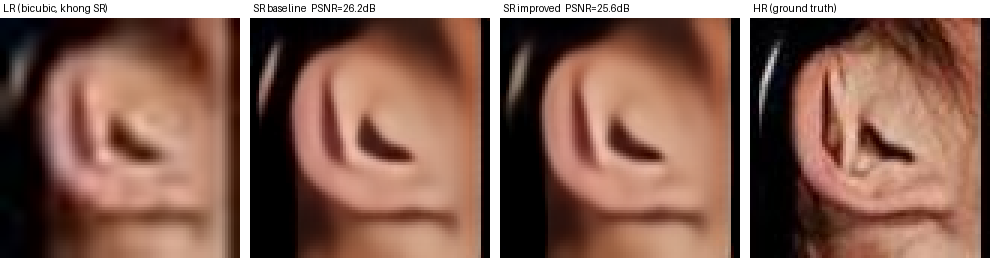
\includegraphics[width=0.48\textwidth]{figures/sample_03.png}\\[0.5mm]
{\footnotesize (b) baseline 30.920\,dB/SSIM 0.8580, span\_tiny 30.890\,dB/SSIM 0.8544: near-tie, ear largely occluded by hair}\\[1.5mm]
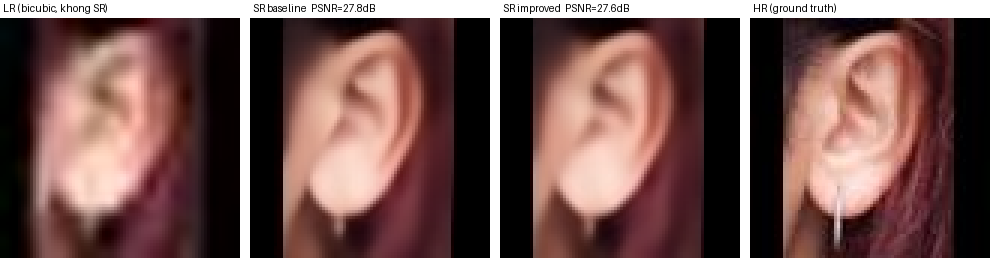
\includegraphics[width=0.48\textwidth]{figures/sample_02.png}\\[0.5mm]
{\footnotesize (c) baseline 25.656\,dB/SSIM 0.8576, span\_tiny 25.252\,dB/SSIM 0.8395: lowest-PSNR pair in the 20-sample export}\\[1.5mm]
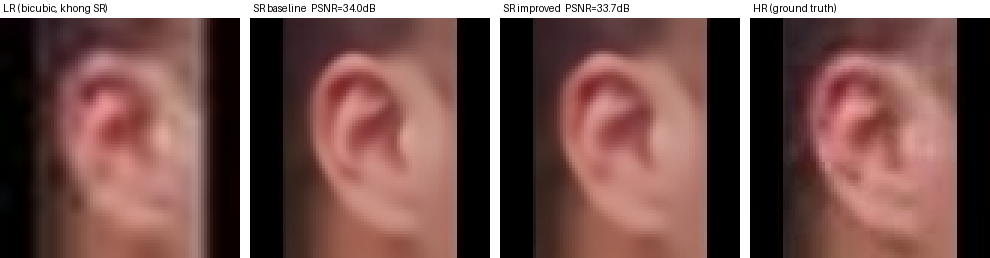
\includegraphics[width=0.48\textwidth]{figures/sample_18.png}\\[0.5mm]
{\footnotesize (d) baseline 34.946\,dB/SSIM 0.9067, span\_tiny 33.716\,dB/SSIM 0.8908: highest-PSNR pair in the 20-sample export}\\[1.5mm]
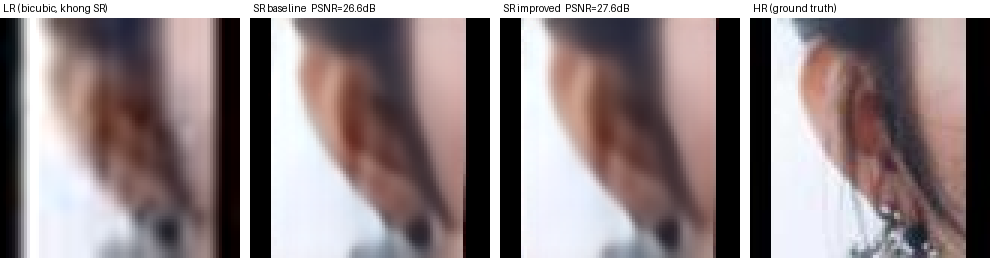
\includegraphics[width=0.48\textwidth]{figures/sample_10.png}\\[0.5mm]
{\footnotesize (e) baseline 31.413\,dB/SSIM 0.9075, span\_tiny 28.768\,dB/SSIM 0.8813: largest observed gap across all 20 exported EarVN1.0 samples}
\caption{Qualitative comparison on five EarVN1.0 test images, each showing (left to right) the bicubic-upsampled LR input (no SR), span\_baseline output, span\_tiny output, and the HR ground truth. Samples (a)--(e) were selected from a 20-sample export to span the full observed per-image PSNR gap, from span\_tiny marginally ahead (a) to the largest gap in favor of span\_baseline (e), together with the lowest- and highest-PSNR pairs observed (c, d), using the exact logged values rather than a curated set of favorable examples.}
\label{fig:qualitative}
\end{figure}

These per-image values are computed over the full image frame, including any letterbox padding, whereas the dataset-level averages in Table~\ref{tab:quality} are computed on the ear region of interest only (Section~\ref{sec:setup}). The two are therefore not directly comparable in absolute terms; the same distinction applies to the AWEx qualitative comparison (Figure~\ref{fig:qualitative-awex}).

\subsection{Ablation: depth (span\_tiny vs.\ span\_large)}
\label{sec:res-depth}

\begin{tableorg}[htbp]
\centering
\caption{span\_tiny vs.\ span\_large, downstream identity accuracy, EarVN1.0, $n=5$ seeds, all eleven recognition backbones. Difference and $d$ are span\_large $-$ span\_tiny; $p_{\text{Bonf}}$ corrected across the 6-comparison family reported by this ablation's own aggregation (Section~\ref{sec:stats}). $p_{\text{TOST}}$ is the equivalence test ($\pm 1$ percentage point margin); ``equiv.'' requires $p_{\text{TOST}}<0.05$, a stricter and distinct claim from ``n.s.''}
\label{tab:depth}

\adjustbox{max width=\textwidth}{\uniformtablesize%
\begin{tabular}{lcccccc}
\toprule
Backbone & span\_tiny & span\_large & Difference & Cohen's $d$ & $p_{\text{Bonf}}$ & $p_{\text{TOST}}$ \\
\midrule
EfficientNet-B0     & 0.5485 & 0.5568 & +0.0083 & 3.17 & 0.0125 (sig.) & 0.11 (not equiv.) \\
GhostNet-100        & 0.5115 & 0.5140 & +0.0025 & 1.33 & 0.244  & \textbf{0.0004 (equiv.)} \\
LCNet-100           & 0.4852 & 0.4966 & +0.0114 & 0.65 & 1.0    & 0.57 (not equiv.) \\
MobileNetV2         & 0.5026 & 0.5044 & +0.0018 & 0.29 & 1.0    & \textbf{0.0235 (equiv.)} \\
MobileNetV3-Large   & 0.5072 & 0.5171 & +0.0099 & 0.41 & 1.0    & 0.50 (not equiv.) \\
MobileNetV3-Small   & 0.4423 & 0.4473 & +0.0050 & 0.37 & 1.0    & 0.23 (not equiv.) \\
MobileOne-S0        & 0.4898 & 0.4837 & $-$0.0060 & $-$0.59 & 1.0 & 0.22 (not equiv.) \\
RegNetY-400MF       & 0.5107 & 0.5147 & +0.0040 & 0.54 & 1.0    & 0.07 (not equiv.) \\
ResNet-18           & 0.4825 & 0.4863 & +0.0038 & 0.45 & 1.0    & 0.09 (not equiv.) \\
ShuffleNetV2-1.0x   & 0.4928 & 0.4923 & $-$0.0005 & $-$0.03 & 1.0 & 0.13 (not equiv.) \\
SqueezeNet-1.1      & 0.4352 & 0.4330 & $-$0.0021 & $-$0.48 & 1.0 & \textbf{0.0087 (equiv.)} \\
\bottomrule
\end{tabular}%
}

\end{tableorg}

10/11 backbones show no statistically significant difference between span\_tiny (0.230M parameters) and span\_large (0.417M parameters). The exception, EfficientNet-B0, shows a small but statistically significant cost ($p_{\text{Bonf}}{=}0.0125$), span\_large ahead by 0.83 percentage points, and this cost is also not confirmed within the equivalence margin by TOST ($p_{\text{TOST}}{=}0.11$), a consistent, real (if small) cost on this backbone by both tests. Of the remaining ten, TOST confirms genuine equivalence within $\pm 1$ percentage point for three (GhostNet-100, $p_{\text{TOST}}{=}0.0004$; MobileNetV2, $p_{\text{TOST}}{=}0.0235$; SqueezeNet-1.1, $p_{\text{TOST}}{=}0.0087$); the other seven (LCNet-100, MobileNetV3-Large, MobileNetV3-Small, MobileOne-S0, RegNetY-400MF, ResNet-18, ShuffleNetV2-1.0x) are non-significant under the paired $t$-test but do not reach the TOST threshold either, and are reported as inconclusive. The paper's central claim is therefore precisely this: reducing depth from 6 to 3 SPABs is confirmed accuracy-neutral in 3/11 backbones, shows a small but real cost in 1/11, and remains an open question at this sample size in the remaining 7/11, not a blanket claim of zero cost everywhere, and stronger where it is made than a non-significance argument alone would support. On AWEx (Section~\ref{sec:res-awex}), the same comparison is statistically non-significant in 11/11 backbones, though at a smaller sample for the original five ($n=3$ seeds) and the standard $n=5$ for the six added later; see Section~\ref{sec:limitations}.

\subsubsection{Locating the compression boundary: a full depth sweep}
\label{sec:depth-sweep}

The comparison above isolates a single point on the depth axis (3 vs.\ 6 blocks) and therefore cannot say how far compression can be pushed before it costs accuracy, only that this particular cut does not. To answer that question directly, span\_tiny's two intermediate block counts (1, 2, 4, 5) were each trained under the identical pinned recipe used for span\_tiny itself (Section~\ref{sec:recipe}, isolating block count as the only varying factor) and evaluated at $n=5$ seeds on MobileNetV2, the representative backbone used for other screening-scale checks in this study, then extended to four further backbones spanning distinct architecture families (ResNet-18, EfficientNet-B0, GhostNet-100, ShuffleNetV2-1.0x) to test whether a compression boundary identified on a single screening backbone generalizes. Figure~\ref{fig:depth-sweep} plots all five backbones' six-point curves together; full mean$\pm$std.\ values and per-point TOST verdicts are in Appendix E, Table~\ref{tab:depth-sweep} and Table~\ref{tab:depth-sweep-pairwise}.

\begin{figure}[htbp]
\centering
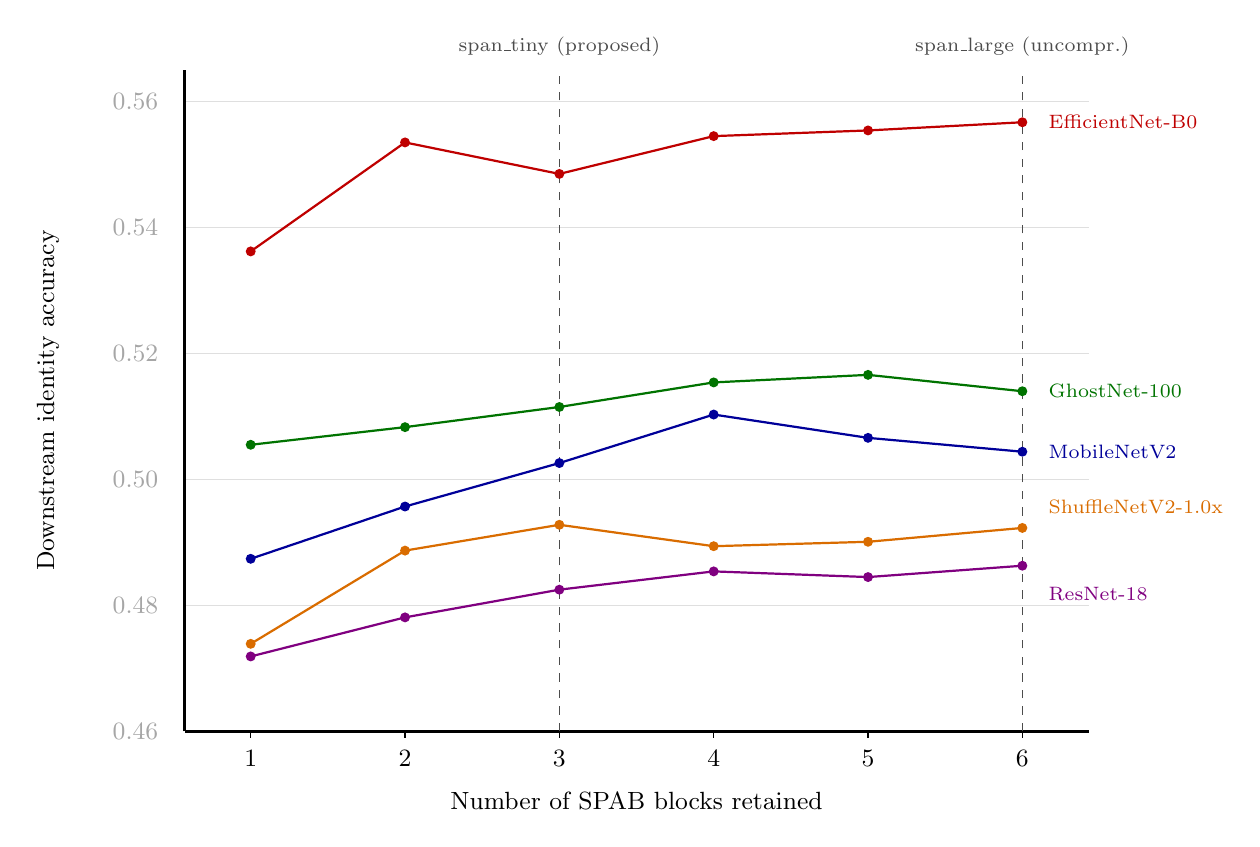
\begin{tikzpicture}[x=1.4cm, y=1cm, font=\small]
    \def\ymin{0}
    \def\ymax{8.4}
    \def\xmin{-0.6}
    \def\xmax{7.6}

    \foreach \acc/\ypos in {0.46/0.0, 0.48/1.6, 0.50/3.2, 0.52/4.8, 0.54/6.4, 0.56/8.0} {
        \draw[gray!25] (\xmin,\ypos) -- (\xmax,\ypos);
        \node[anchor=east, gray!70] at (\xmin-0.15,\ypos) {\acc};
    }

    \draw[thick] (\xmin,\ymin) -- (\xmax,\ymin);
    \draw[thick] (\xmin,\ymin) -- (\xmin,\ymax);

    \foreach \n/\xpos in {1/0.0, 2/1.4, 3/2.8, 4/4.2, 5/5.6, 6/7.0} {
        \draw (\xpos,\ymin) -- (\xpos,\ymin-0.08);
        \node[anchor=north] at (\xpos,\ymin-0.12) {\n};
    }
    \node[anchor=north] at (3.5,\ymin-0.65) {Number of SPAB blocks retained};
    \node[anchor=south, rotate=90] at (\xmin-1.05,4.2) {Downstream identity accuracy};

    \draw[dashed, gray!60!black] (2.8,\ymin) -- (2.8,\ymax);
    \node[anchor=south, gray!60!black, font=\scriptsize] at (2.8,\ymax+0.05) {span\_tiny (proposed)};
    \draw[dashed, gray!60!black] (7.0,\ymin) -- (7.0,\ymax);
    \node[anchor=south, gray!60!black, font=\scriptsize] at (7.0,\ymax+0.05) {span\_large (uncompr.)};

    \draw[thick, blue!60!black]      (0.0,2.192) -- (1.4,2.856) -- (2.8,3.408) -- (4.2,4.024) -- (5.6,3.728) -- (7.0,3.552);
    \draw[thick, red!75!black]       (0.0,6.096) -- (1.4,7.480) -- (2.8,7.080) -- (4.2,7.560) -- (5.6,7.632) -- (7.0,7.736);
    \draw[thick, green!45!black]     (0.0,3.640) -- (1.4,3.864) -- (2.8,4.120) -- (4.2,4.432) -- (5.6,4.528) -- (7.0,4.320);
    \draw[thick, violet]             (0.0,0.952) -- (1.4,1.448) -- (2.8,1.800) -- (4.2,2.032) -- (5.6,1.960) -- (7.0,2.104);
    \draw[thick, orange!85!black]    (0.0,1.112) -- (1.4,2.296) -- (2.8,2.624) -- (4.2,2.352) -- (5.6,2.408) -- (7.0,2.584);

    \foreach \x/\y in {0.0/2.192, 1.4/2.856, 2.8/3.408, 4.2/4.024, 5.6/3.728, 7.0/3.552} { \fill[blue!60!black] (\x,\y) circle (1.8pt); }
    \foreach \x/\y in {0.0/6.096, 1.4/7.480, 2.8/7.080, 4.2/7.560, 5.6/7.632, 7.0/7.736} { \fill[red!75!black] (\x,\y) circle (1.8pt); }
    \foreach \x/\y in {0.0/3.640, 1.4/3.864, 2.8/4.120, 4.2/4.432, 5.6/4.528, 7.0/4.320} { \fill[green!45!black] (\x,\y) circle (1.8pt); }
    \foreach \x/\y in {0.0/0.952, 1.4/1.448, 2.8/1.800, 4.2/2.032, 5.6/1.960, 7.0/2.104} { \fill[violet] (\x,\y) circle (1.8pt); }
    \foreach \x/\y in {0.0/1.112, 1.4/2.296, 2.8/2.624, 4.2/2.352, 5.6/2.408, 7.0/2.584} { \fill[orange!85!black] (\x,\y) circle (1.8pt); }

    \node[anchor=west, blue!60!black, font=\scriptsize] at (7.15,3.552) {MobileNetV2};
    \node[anchor=west, red!75!black, font=\scriptsize] at (7.15,7.736) {EfficientNet-B0};
    \node[anchor=west, green!45!black, font=\scriptsize] at (7.15,4.320) {GhostNet-100};
    \node[anchor=west, violet, font=\scriptsize] at (7.15,1.75) {ResNet-18};
    \node[anchor=west, orange!85!black, font=\scriptsize] at (7.15,2.85) {ShuffleNetV2-1.0x};
\end{tikzpicture}
\caption{Downstream identity accuracy as a function of retained SPAB block count, EarVN1.0, $n=5$ seeds, five backbones (mean values; std.\ dev.\ and per-point TOST verdicts in Table~\ref{tab:depth-sweep} and Table~\ref{tab:depth-sweep-pairwise}). Note the non-monotonic dip for EfficientNet-B0 at exactly 3 blocks (span\_tiny's own choice), and the comparatively flat, low-slope curves for ResNet-18 and ShuffleNetV2-1.0x, for which no block count in the 2--5 range is TOST-confirmed equivalent to the 6-block reference.}
\label{fig:depth-sweep}
\end{figure}

The curve is not monotonic in the range that matters, and this holds across backbones, not only MobileNetV2. Only the most aggressive cut tested, to a single block, produces a cost that reaches significance after Bonferroni correction in three of five backbones (MobileNetV2, EfficientNet-B0, ShuffleNetV2-1.0x), while GhostNet-100 and ResNet-18 show no significant cost even there. EfficientNet-B0's curve is additionally non-monotonic: the 3-block cut (span\_tiny's own choice) shows a significant cost while the \emph{less}-compressed 2-block point does not, a local dip at exactly span\_tiny's chosen depth rather than a clean monotonic decline. GhostNet-100 is the most permissive of the five, TOST-confirmed equivalent to the uncompressed reference from 3 blocks onward; ResNet-18 and ShuffleNetV2-1.0x sit at the opposite end, with no block count in the 2--5 range TOST-confirmed equivalent for either. The confirmed floor of safe compression this study can establish is therefore backbone-dependent rather than a single number: 3 blocks for MobileNetV2 and GhostNet-100 (span\_tiny's own choice, TOST-confirmed equivalent for both), an open question across the entire 2--5 block range for ResNet-18 and ShuffleNetV2-1.0x, and a backbone where the 3-block point specifically underperforms relative to both fewer and more blocks for EfficientNet-B0. This does not change the paper's proposed configuration, since span\_tiny's 3-block design has additionally been validated across all eleven backbones and two datasets (Table~\ref{tab:depth}, Section~\ref{sec:res-awex}); it does show that a full depth curve, even extended across five architecturally distinct backbones, does not settle the compression-boundary question in general: the same $n=5$ statistical-power limitation documented throughout this paper (Section~\ref{sec:limitations}) applies here too.

\subsection{Ablation: loss components}
\label{sec:res-loss}

On MobileNetV2, the six pairwise comparisons among four training-loss configurations (pixel, pixel+distill, pixel+identity, pixel+distill+identity) resolve into two statistically-tied clusters: \{pixel+distill, pixel-only\} both significantly or near-significantly outperform \{pixel+distill+identity, pixel+identity\} (3/4 cross-cluster comparisons significant, 1/4 at trend level), while the two within-cluster comparisons are both non-significant (full results, all eleven backbones, in Appendix G, Table~\ref{tab:loss}). Extending this ablation to ten further backbones shows the pattern is backbone-dependent rather than universal: two backbones echo the same direction (ShuffleNetV2-1.0x at trend level, LCNet-100 at significance on one comparison), while the remaining eight show no comparison reaching even trend level. The standalone $\lambda_{\text{identity}}$ sweep (Section~\ref{sec:recipe}, MobileNetV2-only) corroborates the same negative direction. Read together, the identity-loss term reliably hurts downstream accuracy on MobileNetV2 and, more weakly, on two of the ten other backbones tested, and shows no detectable effect on the remaining eight, a genuinely backbone-dependent effect rather than a general property of the mechanism. By contrast, the distillation term's own marginal contribution (pixel+distill vs.\ pixel-only) remains statistically indistinguishable from pixel-only training on all eleven backbones, TOST-confirmed equivalent on four of them.

\subsection{Contextual comparison with other lightweight SR architectures}
\label{sec:res-context}

Table~\ref{tab:quality} reports SR image-quality metrics for all evaluated architectures, at $n=5$ SR-training seeds for the three core SPAN-family variants and $n=1$ for the rest (Section~\ref{sec:limitations}). Table~\ref{tab:context} reports downstream accuracy comparisons against span\_tiny under the shared Track B distillation recipe, all eleven recognition backbones, $n=5$ seeds.

\begin{tableorg}[htbp]
\centering
\caption{SR image quality on EarVN1.0 (ROI-only, $\times4$). span\_baseline/span\_tiny/span\_large, EDSR, and the four Track-B-distilled contextual architectures (RLFN-adapted, ECBSR, SAFMN, SMFANet) report mean$\pm$std across the same $n=5$ SR-training seeds (42, 123, 2024, 44, 999) used for the SR-seed-variance analysis (Section~\ref{sec:sr-seed-variance}); the Track-A and half-depth rows remain $n=1$ (single training run per configuration, not yet extended to multiple SR-training seeds, Section~\ref{sec:limitations}). MACs/FLOPs are hardware-independent complexity measures (FLOPs $=2\times$MACs), computed once per architecture at a fixed $20\times20$ input resolution and therefore identical across seeds.}
\label{tab:quality}

\adjustbox{max width=\textwidth}{\uniformtablesize%
\begin{tabular}{lccccccc}
\toprule
Model & PSNR (dB) & SSIM & LPIPS$\downarrow$ & Params (M, deploy) & MACs (G) & FLOPs (G) & Latency (ms) \\
\midrule
EDSR (teacher) ($n=5$)                  & 27.385 $\pm$ 0.089 & 0.8293 $\pm$ 0.0023 & 0.1248 $\pm$ 0.0048 & 4.9292 & 1.9699 & 3.9398 & 0.895 \\
span\_baseline ($n=5$)                  & 26.950 $\pm$ 0.317 & 0.8178 $\pm$ 0.0102 & 0.1442 $\pm$ 0.0106 & 0.4263 & 0.1701 & 0.3402 & 0.566 \\
\textbf{span\_tiny} ($n=5$)             & \textbf{27.055 $\pm$ 0.043} & \textbf{0.8196 $\pm$ 0.0012} & \textbf{0.1556 $\pm$ 0.0018} & \textbf{0.230} & \textbf{0.0918} & \textbf{0.1835} & \textbf{0.256} \\
span\_large ($n=5$)                     & 27.191 $\pm$ 0.034 & 0.8243 $\pm$ 0.0009 & 0.1515 $\pm$ 0.0015 & 0.417  & 0.1664 & 0.3328 & 0.464 \\
RLFN (Track A, unmodified, secondary)   & 27.210 & 0.8245 & 0.1379 & 0.3278 & 0.1239 & 0.2479 & 0.684 \\
RLFN-adapted (Track A)                  & 27.192 & 0.8251 & 0.1335 & 0.3278 & 0.1241 & 0.2482 & 0.681 \\
ECBSR (Track A)                         & 26.074 & 0.7883 & 0.1722 & 0.0167 & 0.0067 & 0.0133 & 0.137 \\
SAFMN (Track A)                         & 27.355 & 0.8287 & 0.1350 & 0.2395 & 0.0940 & 0.1881 & 1.824 \\
SMFANet (Track A)                       & 20.906 & 0.6038 & 0.3104 & 0.0844 & 0.0303 & 0.0605 & 1.851 \\
RLFN-adapted (Track B, distilled) ($n=5$) & 27.034 $\pm$ 0.061 & 0.8188 $\pm$ 0.0018 & 0.1539 $\pm$ 0.0015 & 0.3278 & 0.1241 & 0.2482 & 0.710 \\
ECBSR (Track B, distilled) ($n=5$)      & 25.957 $\pm$ 0.070 & 0.7846 $\pm$ 0.0021 & 0.1839 $\pm$ 0.0037 & 0.0167 & 0.0067 & 0.0133 & 0.135 \\
SAFMN (Track B, distilled) ($n=5$)      & 27.217 $\pm$ 0.043 & 0.8243 $\pm$ 0.0014 & 0.1516 $\pm$ 0.0025 & 0.2395 & 0.0940 & 0.1881 & 1.799 \\
SMFANet (Track B, distilled) ($n=5$)    & 26.330 $\pm$ 0.108 & 0.7967 $\pm$ 0.0038 & 0.1812 $\pm$ 0.0065 & 0.0844 & 0.0303 & 0.0605 & 1.878 \\
SAFMN half-depth (Track B, distilled)   & 27.002 & 0.8176 & 0.1564 & 0.1281 & 0.0503 & 0.1007 & 1.103 \\
SMFANet half-depth (Track B, distilled) & 26.140 & 0.7900 & 0.1935 & 0.0477 & 0.0173 & 0.0347 & 1.125 \\
\bottomrule
\end{tabular}%
}

\end{tableorg}

Within the SPAN family itself, span\_tiny's mean PSNR (27.055$\pm$0.043\,dB) is nominally higher than span\_baseline's (26.950$\pm$0.317\,dB) despite roughly half the parameters, a gap smaller than it first appears once span\_baseline's substantially larger seed-to-seed variance is accounted for (nearly $7\times$ span\_tiny's standard deviation), and plausibly related to span\_baseline's fine-tuning from a fixed pretrained initialization (Section~\ref{sec:arch}) into a $20\times20$-input regime well outside that pretraining's original design range, versus span\_tiny's from-scratch training specifically for this resolution; this is offered as a plausible account of the direction, not a confirmed mechanism, and does not affect the compression-safety claim, which concerns downstream accuracy rather than PSNR. span\_tiny is the second-fastest model, behind only ECBSR, and third-smallest by parameter count and by MACs/FLOPs alike, behind ECBSR and SMFANet on both hardware-independent measures. On PSNR, extending the four Track-B contextual architectures to the same $n=5$ SR-training seeds as span\_tiny (rather than the single run used in an earlier comparison) gives a closer picture than a point estimate alone suggested: span\_tiny (27.055$\pm$0.043\,dB) and RLFN-adapted (27.034$\pm$0.061\,dB) are statistically indistinguishable point estimates, both behind only SAFMN (27.217$\pm$0.043\,dB) and both clearly ahead of SMFANet (26.330$\pm$0.108\,dB) and ECBSR (25.957$\pm$0.070\,dB). span\_tiny's PSNR is therefore not top-ranked, but it is no longer accurate to call it low-ranked either; as Table~\ref{tab:context} shows next, its downstream-accuracy standing (tied with the top two, significantly ahead of the bottom two) now broadly tracks this PSNR grouping rather than contradicting it, though the two measures are not identical: span\_tiny's case rests on matching the top performers at a fraction of their parameter count and latency, not on outranking them on either metric. SMFANet's pixel-loss-only (Track A) result (20.906\,dB, still $n=1$) was investigated directly rather than assumed to be an error. The checkpoint itself was confirmed healthy, and the low score reflects SMFANet's difficulty converging under pure pixel supervision at 20$\times$20 resolution. With distillation supervision (Track B), SMFANet recovers to 26.330\,dB (+5.4\,dB), and Track B results are therefore used for all comparative claims involving SMFANet. The half-depth SAFMN/SMFANet rows support the attention-parameterization ablation (Section~\ref{sec:extended-ablations}).

\begin{tableorg}[htbp]
\centering
\caption{span\_tiny vs.\ four other Track-B lightweight SR architectures, downstream accuracy, EarVN1.0, all eleven recognition backbones, $n=5$ seeds. $d$ is span\_tiny minus the other architecture (positive $=$ span\_tiny ahead); $p_{\text{Bonf}}$ corrected across the 6-comparison family reported by each backbone's own aggregation (Section~\ref{sec:stats}). ``(equiv.)'' indicates TOST-confirmed equivalence within $\pm 1$ percentage point.}
\label{tab:context}

\adjustbox{max width=\textwidth}{\uniformtablesize%
\begin{tabular}{lcccc}
\toprule
Backbone & vs.\ RLFN-adapted & vs.\ SAFMN & vs.\ ECBSR & vs.\ SMFANet \\
\midrule
EfficientNet-B0     & $d{=}{-}0.79$, n.s.\ & $d{=}{-}0.89$, n.s.\ & $d{=}{+}3.37$, \textbf{sig.} & $d{=}{+}6.97$, \textbf{sig.} \\
GhostNet-100        & $d{=}{-}0.98$, n.s.\ & $d{=}{+}0.24$, n.s.\ (tiny ahead, equiv.) & $d{=}{+}2.94$, \textbf{sig.} & $d{=}{+}2.30$, \textbf{sig.} \\
LCNet-100           & $d{=}{-}0.15$, n.s.\ (equiv.) & $d{=}{-}0.39$, n.s.\ & $d{=}{+}2.72$, \textbf{sig.} & $d{=}{-}0.14$, n.s.\ \\
MobileNetV2         & $d{=}{-}0.17$, n.s.\ & $d{=}{-}0.24$, n.s.\ (equiv.) & $d{=}{+}3.79$, \textbf{sig.} & $d{=}{+}2.08$, trend \\
MobileNetV3-Large   & $d{=}{-}0.14$, n.s.\ (equiv.) & $d{=}{-}0.69$, n.s.\ & $d{=}{+}0.73$, n.s.\ & $d{=}{+}2.56$, \textbf{sig.} \\
MobileNetV3-Small   & $d{=}{-}0.22$, n.s.\ & $d{=}{+}0.11$, n.s.\ (tiny ahead) & $d{=}{+}2.41$, \textbf{sig.} & $d{=}{+}1.37$, n.s.\ (tiny ahead) \\
MobileOne-S0        & $d{=}{+}0.17$, n.s.\ (tiny ahead) & $d{=}{+}1.10$, n.s.\ (tiny ahead) & $d{=}{+}1.65$, n.s.\ & $d{=}{+}1.28$, n.s.\ (tiny ahead) \\
RegNetY-400MF       & $d{=}{+}0.07$, n.s.\ (tiny ahead, equiv.) & $d{=}{+}0.53$, n.s.\ (tiny ahead) & $d{=}{+}4.39$, \textbf{sig.} & $d{=}{+}2.47$, \textbf{sig.} \\
ResNet-18           & $d{=}{-}0.56$, n.s.\ & $d{=}{+}0.18$, n.s.\ (tiny ahead, equiv.) & $d{=}{+}1.85$, trend & $d{=}{+}1.49$, n.s.\ (tiny ahead) \\
ShuffleNetV2-1.0x   & $d{=}{-}0.18$, n.s.\ & $d{=}{-}0.02$, n.s.\ (equiv.) & $d{=}{+}2.97$, \textbf{sig.} & $d{=}{+}1.77$, trend \\
SqueezeNet-1.1      & $d{=}{-}0.11$, n.s.\ (equiv.) & $d{=}{-}0.69$, n.s.\ & $d{=}{+}2.61$, \textbf{sig.} & $d{=}{+}2.11$, trend \\
\bottomrule
\end{tabular}%
}

\end{tableorg}

Across all eleven backbones, span\_tiny is never significantly beaten by any of the four architectures compared. Against RLFN-adapted, span\_tiny is statistically tied in 11/11 backbones, nominally ahead in 2/11 (MobileOne-S0, RegNetY-400MF), and TOST confirms genuine equivalence in 4/11 (LCNet-100, MobileNetV3-Large, RegNetY-400MF, SqueezeNet-1.1, $p_{\text{TOST}}$ 0.0047--0.0382); the remaining 7/11 are tied but not TOST-confirmed, so that comparison stays an open, underpowered question for those backbones rather than a confirmed tie. Against SAFMN, span\_tiny is likewise tied in 11/11, nominally ahead in 5/11 (GhostNet-100, MobileNetV3-Small, MobileOne-S0, RegNetY-400MF, ResNet-18), and TOST-confirmed equivalent in 4/11 (GhostNet-100, MobileNetV2, ResNet-18, ShuffleNetV2-1.0x, $p_{\text{TOST}}$ 0.0025--0.0401). Against ECBSR, span\_tiny wins with significance in 8/11 backbones, at trend level in a ninth (ResNet-18, $p_{\text{Bonf}}{=}0.0862$), and is statistically tied in the remaining two (MobileNetV3-Large, MobileOne-S0), the first backbones in this comparison, across either the original five or the six added later, where span\_tiny does not clearly beat ECBSR. Against SMFANet, span\_tiny wins with significance in 4/11, at trend level in 3/11 (MobileNetV2, ShuffleNetV2-1.0x, SqueezeNet-1.1), and is tied in the remaining 4/11, nominally ahead in three of those (MobileNetV3-Small, MobileOne-S0, ResNet-18) and nominally (non-significantly) behind in one (LCNet-100). This broadly tracks, rather than contradicts, the PSNR/SSIM picture in Table~\ref{tab:quality} once all five architectures are measured at the same $n=5$ standard (span\_tiny statistically indistinguishable from RLFN-adapted, both behind only SAFMN, both clearly ahead of ECBSR/SMFANet): on the metric the paper is actually organized around, span\_tiny is competitive with the best-performing alternatives and significantly outperforms the two weakest ones in most, though no longer quite all, backbones. The stronger evidence in this paper that pixel-fidelity metrics are an imperfect proxy for recognition-relevant SR quality comes not from this cross-architecture ranking but from the qualitative, within-image analysis (Section~\ref{sec:res-main}), where a near-tied PSNR is shown to be driven by accurate reconstruction of hair and background rather than the ear region the recognition task actually depends on. This comparison remains contextual to the paper's central claim (Sections~\ref{sec:res-main}--\ref{sec:res-depth}), which concerns depth compression \emph{within} the SPAN family, not a claim that span\_tiny is the best-performing lightweight SR architecture in absolute terms.

\subsection{Auxiliary validation: real low-resolution holdout}
\label{sec:res-lr-holdout}

On a held-out set of 173 genuinely low-resolution ear images (rather than synthetically downsampled ones), an initial screen on mobilenet\_v2 alone found that downstream accuracy \emph{reverses} the main result's ordering (no-SR scoring above both SR variants). Extending this check to all eleven recognition backbones (Appendix H, Table~\ref{tab:lr-holdout}), at $n=5$ seeds each, shows this reversal is \emph{not} a general property of the real-low-resolution regime: only 3 of 11 backbones show the reversal direction at all, and of these only one reaches this paper's significance threshold, ResNet-18 ($d{=}{-}1.84$, $p_{\text{Bonf}}{=}0.044$); two backbones (MobileNetV3-Small, LCNet-100) trend in the \emph{opposite} direction, SR nominally helping. This argues against the reversal being a property of the images or the SR output themselves: all eleven backbones see the exact same 173 images and reconstructions, so a uniform artifact would produce a uniform direction, and it does not. \texttt{span\_tiny} vs.\ \texttt{span\_baseline} itself remains non-significant on every backbone (not tabulated separately), consistent with the compression-safety claim holding on this holdout too, independent of whether a given backbone shows the reversal.

The likely mechanism is a resolution mismatch: every one of the 173 holdout images has a native short side strictly below 20\,px, below what the SR models were trained to receive as input, so a model trained to confidently reconstruct fine detail from one specific, clean synthetic degradation can hallucinate plausible-looking but incorrect high-frequency structure, whereas plain bicubic upsampling (no-SR) never attempts this reconstruction, a known failure mode of models trained on synthetic degradation transferring poorly to real-world degradation. This hallucination risk is not uniformly harmful: ResNet-18 is the only backbone with a statistically solid reversal, and is independently the one backbone flagged elsewhere in this paper (Section~\ref{sec:res-awex-transfer}) as not fitting the compression-safety pattern cleanly on AWEx's frozen-backbone-transfer protocol, a completely different dataset and distribution shift, yet the same backbone stands out under both, consistent with a general-fragility account: of the eleven backbones, ResNet-18 alone uses full (non-depthwise-separable) convolutions and predates the mobile-efficiency-driven design choices common to the other ten. Two more specific candidate accounts were checked and did not hold up (architecture family does not cleanly separate the reversing backbones from the rest; the magnitude of a backbone's own clean-data SR benefit does not predict reversal). This general-fragility account is offered as the most consistent candidate explanation, not a confirmed mechanism, and is discussed further as a boundary condition on the paper's central claim in Section~\ref{sec:limitations} rather than evidence against it, since the main claim concerns the synthetic bicubic-downsampling regime (Section~\ref{sec:method}), not arbitrary real-world low-resolution images. Gender accuracy on this holdout, and a crossed-seed replication check, remain MobileNetV2-only observations pending further work.

\subsubsection{Mitigation for the boundary condition: degradation-augmented training}
\label{sec:degradation-mitigation}

Rather than leaving the resolution-mismatch boundary condition as an unaddressed limitation, a direct mitigation was implemented and tested: both span\_tiny and span\_baseline were retrained with the LR input generated by a randomized real-world-style degradation pipeline (Gaussian blur, additive noise, and JPEG compression) rather than clean bicubic downsampling alone, following the classical degradation-modeling approach used in BSRGAN~\cite{zhang2021designing} rather than the more elaborate two-stage pipeline of Real-ESRGAN~\cite{wang2021realesrgan}. Only the training-time LR generation changes; the validation split, the distillation recipe, and the frozen teacher are unchanged, isolating the effect of degradation diversity specifically. This retraining does not disturb the paper's central claim, on the original screening backbone (MobileNetV2) and four further backbones (ResNet-18, EfficientNet-B0, GhostNet-100, ShuffleNetV2-1.0x): no significant span\_tiny-vs-span\_baseline difference for four of five, a trend-level cost for the fifth (EfficientNet-B0, already flagged as an exception under the original recipe, Table~\ref{tab:depth}); TOST does not confirm equivalence for any of the five, consistent with the corresponding EarVN1.0 backbones in Table~\ref{tab:main} (full statistics in Appendix I, Table~\ref{tab:degradation-sanity}).

Re-evaluated on the same 173-image real-low-resolution holdout (full results in Appendix I, Tables~\ref{tab:degradation-holdout}--\ref{tab:degradation-holdout-pairwise-newbackbones}), the mitigation's effect is asymmetric and backbone-dependent. On the original screening backbone (MobileNetV2): span\_baseline does not benefit, and on gender accuracy the gap to no-SR becomes significantly \emph{worse} than under the original recipe ($d{=}{-}3.08$ vs.\ $d{=}{-}1.43$); span\_tiny instead shows a consistent, if not individually significant, improvement on both metrics, including a reversal to nominally beating no-SR on gender accuracy (0.8509 vs.\ 0.8451). A candidate mechanism for this asymmetry (that span\_baseline's larger capacity permits more confident, incorrect high-frequency reconstruction under distribution shift) was tested via a paired Laplacian-variance sharpness analysis across all 173 images and found no support: the paired effect between the two architectures is negligible under both recipes, and sharpness gain correlates \emph{positively}, not negatively, with identity accuracy (Spearman $\rho{=}0.20$), the opposite of what the account predicts; the cause of the asymmetry is left open.

Extended to four further backbones, the mitigation's effectiveness is itself backbone-dependent: two backbones (GhostNet-100, ShuffleNetV2-1.0x) show no reversal at all, with SR now significantly \emph{helping} both span\_baseline and span\_tiny; EfficientNet-B0 shows no effect in either direction. ResNet-18 is the one backbone where the mitigation clearly does not help: span\_baseline remains significantly worse than no-SR on both identity and gender accuracy even under the degradation-augmented recipe, with span\_tiny nominally, but not significantly, closer. This is the same backbone identified above as the only one with a statistically solid reversal under the \emph{original} recipe, and the same backbone independently flagged elsewhere (Section~\ref{sec:res-awex-transfer}) as not fitting the compression-safety pattern cleanly on AWEx's frozen-backbone-transfer protocol: a mitigation designed and validated on one screening backbone does not automatically transfer to the specific backbone independently identified as most fragile to this class of distribution shift, itself informative: whatever makes ResNet-18 more sensitive to the resolution mismatch is not remedied by more diverse synthetic degradation alone, at least not under the recipe tested here.

\subsection{Cross-dataset generalization (AWEx)}
\label{sec:res-awex}

All AWEx results below were generated after every correction described in Section~\ref{sec:integrity} and every statistical-methodology refinement described in Section~\ref{sec:stats} had already been incorporated; no AWEx figure from an earlier, uncorrected stage of this study is reused anywhere in this paper.

\subsubsection{From-scratch track}

Models were trained from scratch on AWEx (no transfer of weights or teacher checkpoints from EarVN1.0), across all eleven recognition backbones (full per-backbone results in Appendix J, Table~\ref{tab:awex-scratch}). \texttt{tiny vs.\ baseline} is non-significant in 11/11 backbones, TOST-confirmed equivalent within $\pm 1$ percentage point for 2 (MobileNetV2, MobileNetV3-Small); the remaining 9 are non-significant without being confirmed equivalent. \texttt{baseline}$>$\texttt{lr} reaches significance in 7/11 backbones and trend level in one more; \texttt{tiny}$>$\texttt{lr} reaches significance in 5/11 and trend level in one more. \texttt{span\_tiny} vs.\ \texttt{span\_large} on this track shows no statistically significant difference in 11/11 backbones (Section~\ref{sec:res-depth}), further corroborating the depth-compression finding on a second, independent dataset. An earlier stage of this study, predating the corrections in Section~\ref{sec:integrity}, had reported an off-trend ResNet-18 result on this track; this does not replicate under the corrected setup and is not carried forward as a limitation.

An HR-ceiling check identical in protocol to Section~\ref{sec:hr-ceiling} was also run on AWEx (from-scratch track, $n=5$ seeds, all eleven backbones; full table in Appendix J, Table~\ref{tab:awex-hr-ceiling}). The pattern is far weaker and noisier than on EarVN1.0, consistent with AWEx's already-documented small per-subject sample size (Section~\ref{sec:disc-power}): \texttt{hr}$>$\texttt{lr} reaches significance in 7 of 11 backbones, and \texttt{hr} vs.\ \texttt{span\_tiny} in only 2 of 11, both behaving as a ceiling should. One backbone (MobileNetV3-Small) shows a trend-level reversal instead (\texttt{span\_tiny} nominally above the \texttt{hr} ceiling); this was investigated directly rather than left unexamined: confusion-matrix recomputation rules out a computation error, and training logs show \texttt{hr}'s validation-to-test generalization gap is roughly five times larger than \texttt{span\_tiny}'s on this backbone, consistent with the classification head overfitting AWEx's very small per-subject validation split when trained directly on uncompressed images, not evidence that a super-resolved image carries more identity information than its source. This AWEx check is read as a weaker-power replication of the EarVN1.0 finding, not a contradiction of it: every backbone reaching significance on any ceiling comparison agrees with the expected direction, and the one reversal does not itself reach significance.

Appendix J, Table~\ref{tab:awex-quality} reports SR image quality for the from-scratch track: all four models score within a coherent 24.5--25.6\,dB band with no anomaly, in contrast to an earlier stage of this study in which \texttt{span\_large} had scored anomalously low with no corresponding downstream-accuracy effect, an anomaly not present under the current measurements. The contextual comparison against RLFN/ECBSR/SAFMN/SMFANet (Table~\ref{tab:quality}, Table~\ref{tab:context}) was run on EarVN1.0 only in this phase of the study; extending it to AWEx is noted as a direction for future work (Section~\ref{sec:limitations}).

\subsubsection{Transfer-learning tracks (primary result for AWEx)}
\label{sec:res-awex-transfer}

Given AWEx's smaller per-subject sample size, two transfer-learning protocols initialized from EarVN1.0-trained weights are evaluated: full fine-tuning of the entire recognition backbone, and a frozen-backbone variant that only fine-tunes the classification head. Both are reported as primary results, because they answer a related but distinct question and do not agree in every respect (full per-backbone results in Appendix J, Table~\ref{tab:awex-transfer} and Table~\ref{tab:awex-transfer-frozen}).

Under full fine-tuning, \texttt{span\_baseline} $>$ \texttt{lr} reaches significance in 8/11 backbones and trend level in a ninth, and \texttt{span\_tiny} $>$ \texttt{lr} in 3/11. Critically for this paper's central claim, \texttt{span\_tiny} vs.\ \texttt{span\_baseline} is non-significant in 11/11 backbones. TOST does not confirm genuine equivalence for any of the eleven backbones under this protocol, a weaker showing than the from-scratch track's 2/11 confirmed; the finding replicates at the ``not detected as significant'' level across all eleven.

Under the frozen-backbone protocol, \texttt{span\_baseline} $>$ \texttt{lr} reaches significance in 6/11 backbones and trend level in two more; \texttt{span\_tiny} $>$ \texttt{lr} reaches significance in 5/11. As with full fine-tuning, \texttt{span\_tiny} vs.\ \texttt{span\_baseline} reaches this paper's significance threshold in 0/11 backbones, with one at trend level (not TOST-confirmed). The compression-safety finding is therefore confirmed, at the ``not detected as significant'' strength, under both transfer protocols and the from-scratch track alike: 0/11 backbones show a significant accuracy cost from compression under any of the three protocols tested on AWEx; genuine equivalence is TOST-confirmed for 2 of the 33 backbone$\times$protocol combinations overall. The two protocols disagree on secondary detail (under frozen backbone, \texttt{span\_tiny} is nominally above \texttt{span\_baseline} in 4/11 backbones, never significantly), but ResNet-18 remains, across all three AWEx protocols and now across all eleven backbones, the one case where \texttt{span\_tiny} falls nominally below \texttt{lr} under any protocol, a backbone-specific limitation (Section~\ref{sec:limitations}), not evidence against the compression-safety claim.

An identical real-low-resolution-holdout check to Section~\ref{sec:res-main} was also run on AWEx (mobilenet\_v2, frozen-backbone checkpoints, $n=1$): no-SR $=0.0$, span\_baseline$=0.0625$, span\_tiny$=0.0938$. Unlike the EarVN1.0 holdout, both SR variants clearly beat no-SR here rather than reversing it; span\_tiny is nominally ahead of span\_baseline. With $n=1$ and only 32 images (Section~\ref{sec:limitations}), this is not treated as contradicting the EarVN1.0 finding, only as insufficient evidence on its own either way.

Figure~\ref{fig:qualitative-awex} shows qualitative examples on AWEx test images, from the transfer-learning track (full fine-tuning protocol, Table~\ref{tab:awex-transfer}), using the SR checkpoints fine-tuned specifically for that protocol. Across the 15 exported AWEx test samples, the per-image PSNR gap (span\_baseline $-$ span\_tiny) ranges from $-0.042$\,dB (sample index 13, span\_tiny fractionally ahead) to $+1.358$\,dB (sample index 8, the largest gap observed), a narrower range than in an earlier export tied to a different (frozen-backbone) checkpoint, consistent with this being a genuinely different SR checkpoint rather than a re-labeling of the same one. The five panels shown are selected by PSNR-gap quartile across the full 15-sample export (minimum, Q1, median, Q3, maximum) rather than by visual inspection, so the selection is not biased toward either model; none of the five is grayscale.

\begin{figure}[htbp]
\centering
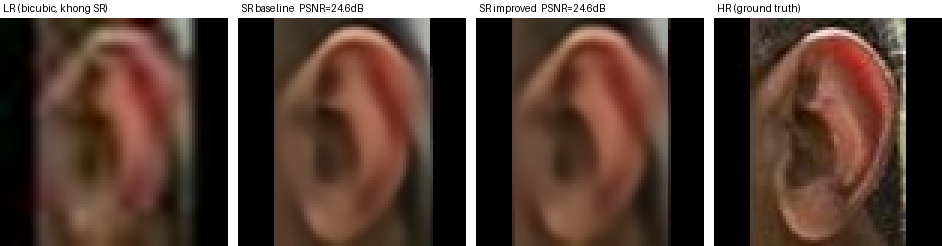
\includegraphics[width=0.48\textwidth]{figures_awex/sample_13.png}\\[0.5mm]
{\footnotesize (a) baseline 24.602\,dB/SSIM 0.7787, span\_tiny 24.644\,dB/SSIM 0.7733: span\_tiny marginally ahead, minimum gap observed}\\[1.5mm]

\includegraphics[width=0.48\textwidth]{figures_awex/sample_03.png}\\[0.5mm]
{\footnotesize (b) baseline 25.318\,dB/SSIM 0.8643, span\_tiny 25.092\,dB/SSIM 0.8557: gap 0.226\,dB (Q1)}\\[1.5mm]
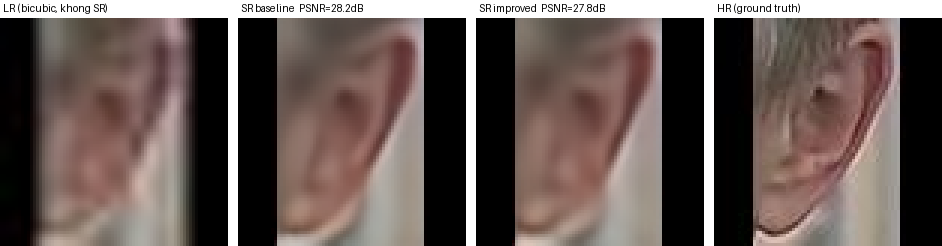
\includegraphics[width=0.48\textwidth]{figures_awex/sample_14.png}\\[0.5mm]
{\footnotesize (c) baseline 28.190\,dB/SSIM 0.8278, span\_tiny 27.827\,dB/SSIM 0.8168: gap 0.363\,dB (median)}\\[1.5mm]
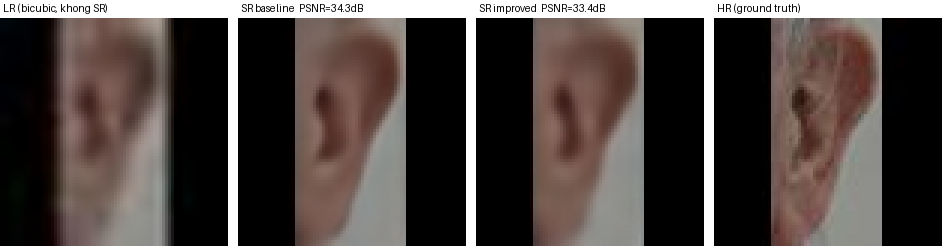
\includegraphics[width=0.48\textwidth]{figures_awex/sample_00.png}\\[0.5mm]
{\footnotesize (d) baseline 34.258\,dB/SSIM 0.9302, span\_tiny 33.351\,dB/SSIM 0.9218: gap 0.907\,dB (Q3)}\\[1.5mm]
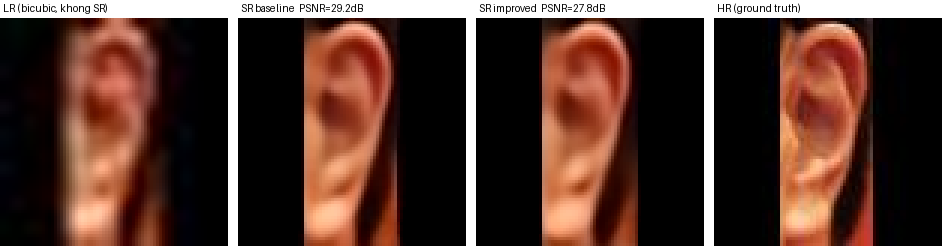
\includegraphics[width=0.48\textwidth]{figures_awex/sample_08.png}\\[0.5mm]
{\footnotesize (e) baseline 29.204\,dB/SSIM 0.8962, span\_tiny 27.846\,dB/SSIM 0.8745: largest gap observed across all 15 exported AWEx samples}
\caption{Qualitative comparison on five AWEx test images, each showing (left to right) the bicubic-upsampled LR input (no SR), span\_baseline output, span\_tiny output, and the HR ground truth. Samples (a)--(e) are selected by PSNR-gap quartile (minimum, Q1, median, Q3, maximum) across the 15-sample export, from span\_tiny marginally ahead (a) to the largest gap in favor of span\_baseline (e).}
\label{fig:qualitative-awex}
\end{figure}
\FloatBarrier

The paper's central compression-safety claim (\texttt{span\_tiny} statistically indistinguishable from \texttt{span\_baseline}) is confirmed on a second, independent dataset under \emph{three} separate protocols (from-scratch, full-fine-tune transfer, frozen-backbone transfer), with 0/11 backbones showing a significant cost under any of them; equivalence testing (TOST) confirms this is genuinely negligible for 2 of the 33 backbone$\times$protocol combinations (MobileNetV2 and MobileNetV3-Small, both on the from-scratch track), with the remainder reported as not detected as significant rather than confirmed safe. The secondary question, whether SR helps over no-SR at all, is directionally positive across most backbone$\times$protocol combinations but noisier and protocol-dependent in exactly which backbones reach significance, consistent with AWEx's smaller per-subject training sample ($\approx$6.7 images/subject vs.\ substantially more on EarVN1.0) rather than a contradiction of the EarVN1.0 findings; this distinction is discussed further in Section~\ref{sec:disc-power}. ResNet-18 is the one backbone that does not fit this pattern cleanly on AWEx (Section~\ref{sec:res-awex-transfer}), a limitation discussed further in Section~\ref{sec:limitations}.

\subsection{Additional mechanisms tested for further improvement: a negative-result ablation study}
\label{sec:novelty-ablations}

None of the three candidate mechanisms for improving span\_tiny's downstream accuracy further (a richer distillation loss, a saliency-weighted identity-critical loss, and learned/differentiable block pruning as an alternative to span\_tiny's fixed, hand-picked block selection) improves on the main recipe. Each was screened at reduced scale first, then validated to the same statistical standard as the main result ($n=5$ seeds, all eleven recognition backbones, EarVN1.0).

\subsubsection{Feature-level distillation (``KD v2'')}

This mechanism adds a feature-level distillation term (matching intermediate SPAN features between student and teacher) to the existing pixel+distillation recipe (Appendix A, Table~\ref{tab:kdv2-ablation}). No backbone shows a statistically significant difference in either direction, and the sign of the effect is inconsistent across backbones (positive in 5/11, negative in 6/11), with small effect sizes centered near zero, a genuine absence of effect rather than an underpowered trend.

\subsubsection{Saliency-weighted identity-critical loss}

This mechanism reweights the pixel-reconstruction loss by a saliency map derived from identity-relevant image regions, intended to concentrate SR fidelity where it matters most for recognition (Appendix B, Table~\ref{tab:saliency-ablation}). Again no backbone reaches significance, with a positive trend in 9/11 backbones that never clears Bonferroni correction.

\subsubsection{Learned/differentiable block pruning}

Rather than span\_tiny's fixed choice to keep the first three of six SPABs, this mechanism learns which blocks to keep via a differentiable gating mechanism with a sparsity penalty, in the same general family as scaling-factor-based structured pruning (Network Slimming~\cite{liu2017slimming}) applied at block granularity. At the sparsity level matching span\_tiny's parameter count exactly (0.230M, 3 blocks), learned pruning is significantly \emph{worse} than the fixed, hand-picked selection in 10/11 backbones, with large effect sizes throughout ($d$ $-$2.1 to $-$6.0); the one exception, MobileNetV3-Large, is non-significant rather than reversed (Appendix C, Table~\ref{tab:pruning-ablation}). A negative result for the differentiable-pruning mechanism specifically, not for depth compression in general, which Table~\ref{tab:depth} shows is close to accuracy-neutral when the retained blocks are chosen by hand.

Summarizing across the three: feature-level distillation and the saliency-weighted loss are statistically null in either direction, and learned pruning is significantly negative in the large majority of backbones. The paper's validated contribution remains span\_tiny's original depth-count reduction (Sections~\ref{sec:res-main}--\ref{sec:res-depth}).

\subsection{Extended ablations toward mechanistic and design generality}
\label{sec:extended-ablations}

The results above establish that depth compression is accuracy-neutral for span\_tiny specifically. Three further questions were identified to test whether this finding reflects a general mechanism or an architecture-specific coincidence, and whether the specific design choices made for span\_tiny are themselves well-supported. All three have now been run to completion, on EarVN1.0, to the same $n=5$-seed standard as the main result and extended to all eleven recognition backbones: the first (attention-parameterization) and third (block-removal position) directly, and the second (recognition-embedding-space distillation) by recognizing, on inspection, that it already has an answer from an existing result under a different name, described below.

\subsubsection{Attention-parameterization ablation: completed, hypothesis not supported}

Section~\ref{sec:disc-depth} proposes that SPAN tolerates depth reduction because its attention mechanism carries no learned parameters, so removing blocks removes computation but not learned capacity. If this account is correct, an architecture with \emph{learned} attention/modulation should show a measurably larger accuracy cost from an equivalent proportional depth reduction than span\_tiny does. SAFMN~\cite{sun2023safmn} and SMFANet~\cite{zheng2024smfanet}, both using learned modulation mechanisms, were each halved in block count and evaluated under the identical Track B recipe, $n=5$ seeds, all eleven recognition backbones (SR-quality rows in Table~\ref{tab:quality}). Appendix D, Table~\ref{tab:attn-ablation} reports, per backbone, $\Delta_{\text{arch}}$ (that architecture's own full-depth-minus-half-depth accuracy) against $\Delta_{\text{SPAN}}$ (span\_large minus span\_tiny, from Table~\ref{tab:depth}), and a paired test on their difference.

$\Delta_{\text{SPAN}}$ itself ($-$0.0021--0.0114 across backbones, Table~\ref{tab:depth}) is small throughout, and neither SAFMN nor SMFANet loses significantly more than SPAN does from an equivalent proportional depth reduction in \emph{any} of the 22 backbone$\times$architecture combinations tested, all eleven backbones included ($p_{\text{Bonf}}{=}1.0$ throughout). If anything, the diff-of-diffs is negative (SPAN loses as much or more) in 12/22 combinations: SAFMN and SMFANet, despite using learned modulation mechanisms, tolerate an equivalent depth reduction just as well as span\_tiny does, and this null result now holds with zero exceptions across the full eleven-backbone set rather than only the original five. The parameter-free-attention account proposed in Section~\ref{sec:disc-depth} therefore finds no support here and is revised there accordingly: depth tolerance at this compression level and resolution appears to be a broader property of lightweight SR architectures under this training recipe, not a consequence specific to SPAN's parameter-free design.

\subsubsection{Direct test of the low-frequency-signal hypothesis}
\label{sec:freq-ablation}

The ablation above rejects one specific candidate mechanism (fixed, parameter-free attention) but does not itself provide positive evidence for the replacement account proposed in its place (Section~\ref{sec:disc-depth}): that the recognition-relevant signal in a low-resolution ear crop is concentrated in coarse, low-frequency structure a shallower network already captures. This was tested directly. An FFT-based frequency filter was applied to span\_tiny's SR output, either lowpass (retaining only frequencies below a cutoff) or highpass (retaining only frequencies above it) at eight cutoff levels each, and the filtered images were evaluated with each backbone's already-trained recognition checkpoint (\texttt{recognition\_sr\_improved\_<backbone>}), no retraining, testing what a model trained on unfiltered images actually depends on at inference time, on the full 3480-image EarVN1.0 test set, $n=5$ seeds, all eleven recognition backbones.

\begin{figure}[htbp]
\centering
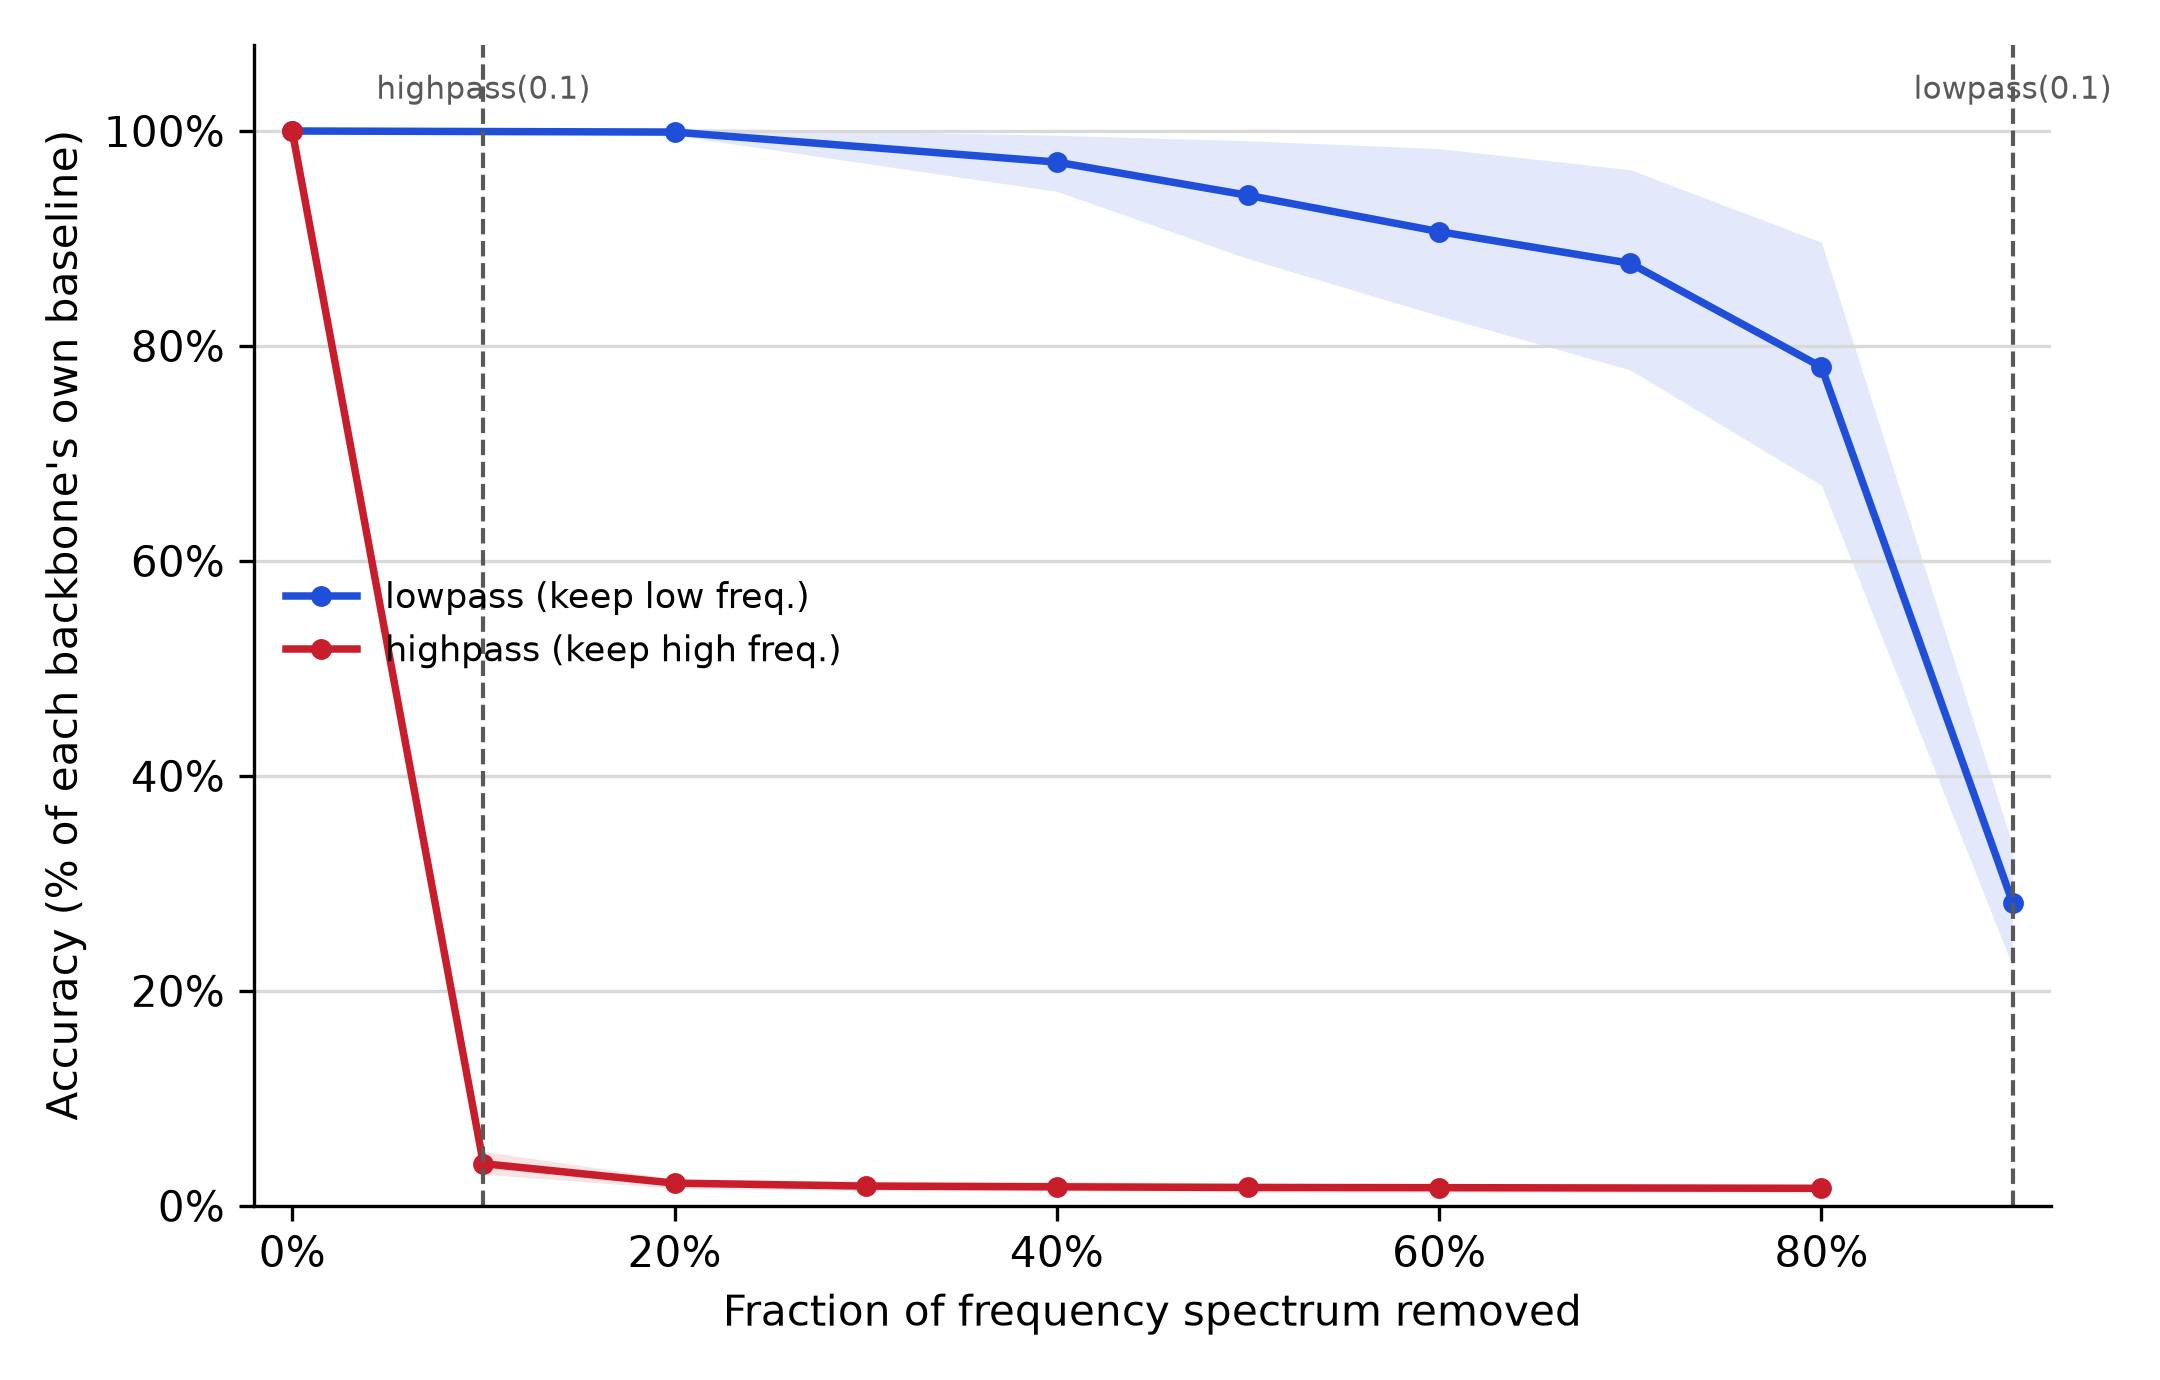
\includegraphics[width=0.85\textwidth]{figures/fig_freq_ablation.png}
\caption{Downstream identity accuracy, normalized to each backbone's own unfiltered baseline ($=100\%$), as a function of the fraction of the frequency spectrum removed, EarVN1.0, $n=5$ seeds, all eleven recognition backbones. Solid lines are the mean across all eleven backbones; shaded bands are the min--max range across backbones at each point; the asymmetry between the two curves holds with zero exceptions, on every backbone tested (per-backbone values at the two labeled cutoffs in Appendix K, Table~\ref{tab:freq-ablation}).}
\label{fig:freq-ablation}
\end{figure}

The two most informative points from the sweep, matched for severity (90\% of the spectrum removed in each direction), are reported per backbone in Table~\ref{tab:freq-ablation}: removing the lowest 10\% of the spectrum (highpass, cutoff 0.1) collapses accuracy to 2.9--5.1\% of the unfiltered baseline across all eleven backbones, near the chance level for this task, while retaining only the lowest 10\% of the spectrum (lowpass, cutoff 0.1) preserves 22.3--33.6\% of baseline accuracy: six to eight times more of each backbone's own baseline survives removing 90\% of the high-frequency content than removing 90\% of the low-frequency content, and this asymmetry holds with zero exceptions across all eleven backbones. The two no-op filter settings (lowpass cutoff$=1.0$, highpass cutoff$=0.0$), computed independently, return identical accuracy for every backbone, a built-in internal consistency check on the filtering pipeline itself. This is a direct confirmation of the low-frequency-signal account: not an inference from a rejected alternative, but a measurement of what an already-trained recognition model's own predictions actually depend on.

A complementary spectral comparison asked the converse question: does depth compression itself remove more high-frequency content than low-frequency content from the SR output? Radially-averaged power spectral density, computed on the same test set across span\_tiny, span\_baseline, span\_large, no-SR, and HR, shows no such asymmetry: span\_tiny's spectrum is nearly indistinguishable from span\_baseline's and span\_large's at every frequency band (summed absolute difference under 0.0003 in each half of the spectrum), smaller than the difference between any of the three SR variants and either the no-SR or HR reference. Depth compression does not measurably alter the frequency content of the SR output itself; the evidence above for the low-frequency-signal account comes from what the recognition model depends on, not from a detectable spectral signature of compression.

\subsubsection{Block-removal position ablation: completed, no significant effect}
\label{sec:position-ablation}

span\_tiny retains the first three of six SPABs (Figure~\ref{fig:arch}), a choice made for implementation convenience rather than validated against alternatives. Two further 3-block variants, holding total block count fixed, test whether removal position matters independently of removal count: one retaining the last three blocks instead (removing blocks 1--3), and one retaining an interleaved subset (blocks 1, 3, 5).

Testing this meaningfully requires more than relabelling a freshly-initialized 3-block network: since span\_tiny is trained end-to-end from a random initialization under output-level distillation only, a 3-block student trained this way has no internal notion of ``which blocks of a virtual 6-block network it occupies''. Three variants trained identically would be expected to differ only by seed noise, not by the position nominally assigned to them. To give position a training signal, each variant instead uses a position-targeted feature-hint loss: the student's final-block output is matched, via a learned $1\times1$ adapter and the same instance-normalized $L_1$ formulation already used for the feature-KD term (Section~\ref{sec:novelty-ablations}), against the teacher's output at a specific block index representing the depth that variant is meant to occupy (block 3 for the current first-three-blocks recipe, block 6 for a last-three-blocks recipe, block 5 for an interleaved 1-3-5 recipe). All three variants use this same mechanism, differing only in which teacher block is targeted, so the comparison isolates position specifically rather than confounding it with the presence or absence of positional supervision. The teacher for this ablation is span\_large rather than span\_baseline/span\_official: both are 6-block, but only span\_large shares the same re-implementation class as span\_tiny (Section~\ref{sec:arch}), giving well-defined intermediate block outputs to target; span\_official's internal structure is external, third-party code without a guaranteed matching interface.

Downstream identity accuracy for the three variants, across all eleven recognition backbones at $n=5$ seeds, is reported in Appendix K, Table~\ref{tab:position-ablation}. None of the three pairwise comparisons reaches significance in any backbone ($p_{\text{Bonf}}$ 0.15--1.0 across all 33 backbone$\times$pair combinations), with effect sizes small throughout. An apparent lean toward keep-last found in an initial five-backbone screen does not hold up as a majority once extended to eleven (keep-last highest in 5/11, keep-first in 2/11, interleaved in 4/11), consistent with this being sampling noise rather than a real trend, now that it is more evenly split, not a weakening of the null result. A separate nominally-significant difference flagged at an initial $n=3$-seed pass (EfficientNet-B0) also did not replicate once extended to $n=5$, the same seed-extension protocol applied throughout this study catching a small-sample false positive before it was reported as a finding. Block-removal position does not detectably affect downstream accuracy at this compression level, on any backbone tested.

\subsubsection{Recognition-embedding-space distillation}

Recognition-aware SR objectives (Ataer-Cansizoglu et al.~\cite{ataer2019identity}; the iris-recognition literature, Section~\ref{sec:related}) suggest aligning the SR loss with a downstream recognition embedding rather than pixel or teacher-feature reconstruction: $\mathcal{L}_{\text{embed}} = 1 - \cos\big(f(\mathrm{SR}(x)),\, f(\mathrm{HR})\big)$, where $f(\cdot)$ is a frozen backbone's penultimate-layer embedding. This is, on inspection, mathematically identical to the identity-loss term already evaluated in Section~\ref{sec:res-loss}: the two configurations it calls for are exactly the pixel+identity and pixel+distill+identity rows already reported in Table~\ref{tab:loss}, not a new experiment. Both fall in the lower-performing cluster there, so the recognition-aware-objective account does not hold in this setting, unlike the face- and iris-recognition results that motivate it.

% ============================================================================
\section{Discussion}
\label{sec:discussion}
% ============================================================================

The design goal of this work was not maximal downstream accuracy but a specific, pre-defined criterion: preserve the ordering \texttt{lr $<$ span\_tiny $<$ span\_baseline} while substantially reducing parameter count and latency, and in particular keep the compression-specific cost (\texttt{span\_tiny} vs.\ \texttt{span\_baseline}) small and, ideally, confirmed negligible. On EarVN1.0 this cost is non-significant in 10/11 backbones (Table~\ref{tab:main}), and TOST equivalence testing confirms 1 of those 10 as negligible at $n=5$ (ShuffleNetV2-1.0x); the depth-isolated comparison (Table~\ref{tab:depth}) gives the cleaner answer, non-significant in 10/11 backbones and TOST-confirmed equivalent in 3 of those 10, with the remaining 7 inconclusive rather than settled. On AWEx it is non-significant in 11/11 backbones under all three protocols tested (from-scratch, full-fine-tune transfer, and frozen-backbone transfer; Section~\ref{sec:res-awex}), the single most consistent result in the paper by the non-significance criterion alone; TOST tells a more modest story there, however, confirming genuine equivalence in only 2 of the 33 backbone$\times$protocol combinations (both on the from-scratch track), with the remainder non-significant but not confirmed negligible. This forms the paper's central empirical claim: no detected cost almost everywhere, confirmed negligible cost in a subset, and an open question in the rest at this sample size.

\label{sec:disc-depth}
Section~\ref{sec:arch} proposed that SPAN tolerates depth reduction because its attention mechanism carries no learned parameters: removing SPABs removes attention \emph{computation} but not learned attention \emph{capacity}, since there is none to lose. This account makes a testable directional prediction (an architecture with \emph{learned} attention/modulation should lose more from an equivalent depth cut), and Section~\ref{sec:extended-ablations} tested it directly against SAFMN and SMFANet, with no exception across every backbone$\times$architecture combination tested. The prediction was not confirmed, so the parameter-free-attention account is not supported by this test and is retracted as the explanation. A more likely account, consistent with both this ablation and the loss-ablation result below, is that at this extreme compression level and input resolution (20$\times$20\,px), the recognition-relevant signal in an ear crop is concentrated in relatively coarse, low-frequency structure that a shallower network already captures adequately, regardless of its attention mechanism's parameterization, making depth reduction broadly tolerable across this class of lightweight SR architectures rather than a property specific to SPAN. Unlike the parameter-free-attention account it replaces, this one was tested directly rather than left as an untested hypothesis: frequency-filtering span\_tiny's SR output and re-evaluating each backbone's already-trained recognition checkpoint shows accuracy depends almost entirely on that low-frequency band, with zero exceptions across all eleven backbones (Section~\ref{sec:freq-ablation}), direct evidence of what the recognition model depends on, rather than an inference from a rejected alternative. A complementary spectral comparison, however, finds no corresponding difference in frequency content between the SR outputs of compressed and uncompressed models themselves, so this account is supported as a description of the recognition model's own input dependence, not as a demonstrated property of what depth compression removes from the image.

Two pieces of evidence here point past SPAN specifically. Depth tolerance holds for two other architecturally distinct designs, SAFMN's spatial modulation and SMFANet's self-modulation, not only SPAN's parameter-free mechanism, and the frequency-dependency result holds across all eleven recognition backbones tested, not a single representative one. Read together, they suggest something broader than either result on its own: once input resolution is pushed this far below what an SR architecture was designed for, how much high-frequency detail it reconstructs may simply stop mattering for a downstream recognition task, because there is little recoverable identity signal left in that band regardless. If that account is correct, it should hold for lightweight SR architectures beyond the three tested here, and for recognition tasks beyond ear biometrics, wherever input resolution is pushed similarly far below design intent. This paper does not test that broader claim: the frequency-domain measurement in Section~\ref{sec:freq-ablation} was performed on span\_tiny's output alone, not on SAFMN's or SMFANet's, so whether their reconstructions show the same frequency-dependency pattern is still open. Checking it would need nothing more than the same filtering procedure applied to a different SR model's output, and would go a good way toward telling apart two possibilities: that depth compression is forgiving at extreme resolutions for reasons that generalize across architectures and tasks, or that the ear-recognition case studied here happens to work out for one dataset and one architecture family.

Section~\ref{sec:res-loss} finds two distinct results that should not be conflated: on MobileNetV2, the identity-loss term \emph{significantly reduces} downstream accuracy (3/6 pairwise comparisons significant, 1/6 at trend level, corroborated independently by the $\lambda_{\text{identity}}$ sweep in Section~\ref{sec:recipe} on the same backbone); extending this ablation to ten further backbones (eleven in total) shows the effect is backbone-dependent rather than universal, echoed more weakly (one at trend level only) on two of the ten (ShuffleNetV2-1.0x, LCNet-100), and undetectable on the remaining eight, so it should be read as a real but backbone-dependent finding rather than either a MobileNetV2-specific artifact or a general property of the mechanism. The distillation term's own marginal contribution, by contrast, remains statistically indistinguishable from pixel-only training across all eleven backbones tested, TOST-confirmed equivalent on four of them (EfficientNet-B0, GhostNet-100, RegNetY-400MF, SqueezeNet-1.1). For the latter, null result, three explanations seem plausible: the pixel-reconstruction signal alone may already be close to sufficient at this parameter scale; seed-to-seed variance may exceed the true effect size; or, as Zhang et al.~\cite{zhang2024dukd} argue for SR distillation generally, a teacher's own output is only an approximation of the true HR image, which caps how much signal the distillation term can supply. The data collected here cannot distinguish between these. Neither result undermines the paper's central claim, which concerns architectural depth, not loss-function choice; span\_tiny's training recipe (Track B, pixel+distillation, $\lambda_{\text{identity}}{=}0$) remains justified independently by its role in stabilizing convergence for other architectures in the contextual comparison (Section~\ref{sec:res-context}) and by the identity-loss ablation's own negative finding for that specific term.

SMFANet failed to converge well under pixel-loss-only supervision (20.906\,dB, Table~\ref{tab:quality}) but recovered strongly under distillation supervision (+5.4\,dB). The marginal contribution of distillation to span\_tiny's own downstream accuracy was not statistically detectable, but this case shows that distillation supervision is not uniformly redundant across architectures at this extreme input resolution. Some architectures appear to depend on it to converge at all.

\label{sec:disc-position}
Beyond the SPAN family, span\_tiny is second-fastest and third-smallest among six compared architectures, and, once all four contextual architectures are measured at the same $n=5$ SR-training-seed standard as span\_tiny (Table~\ref{tab:quality}), is statistically indistinguishable from RLFN-adapted on PSNR/SSIM, both behind only SAFMN and both clearly ahead of ECBSR/SMFANet: not top-ranked, but no longer accurately described as low-ranked either. On downstream recognition accuracy, the metric this paper is organized around, span\_tiny is never significantly beaten by any of the other four architectures across any of the eleven recognition backbones, is statistically tied with the two most accurate ones (RLFN-adapted, SAFMN), and significantly \emph{outperforms} the two least accurate ones in most backbones (ECBSR: 8/11 significant, 1/11 trend, 2/11 tied; SMFANet: 4/11 significant, 3/11 trend, 4/11 tied) (Table~\ref{tab:context}). This PSNR/SSIM grouping and this accuracy grouping now largely agree (SAFMN/RLFN-adapted/span\_tiny cluster together on both, ECBSR/SMFANet trail on both), so the sharper point is not that raw image quality misidentifies span\_tiny specifically, but that it is worth stating plainly what span\_tiny's position does and does not mean: it is not evidence that span\_tiny is the best lightweight SR architecture in absolute terms (SAFMN and RLFN-adapted remain fully competitive, at higher latency for SAFMN and a comparable one for RLFN-adapted), but it is evidence that a compressed architecture can match top-performing, larger alternatives on the metric that actually matters for this task without matching or exceeding them on pixel fidelity. The re-implementation's timing broadly matches the original SPAN paper's comparison against SAFMN on standard SR benchmarks ($\approx$13\,ms/28.66\,dB vs.\ $\approx$72\,ms/$\approx$28.60\,dB on Set14 $\times4$ in~\cite{wan2024span}), an independent data point supporting the general efficiency trade-off observed here, alongside the new evidence that this trade-off does not come at a downstream-accuracy cost relative to the weaker-PSNR alternatives.

\label{sec:disc-power}
The weaker and more protocol-dependent statistical significance of \texttt{SR $>$ lr} on AWEx (Section~\ref{sec:res-awex}) compared to EarVN1.0 (Table~\ref{tab:main}, significant in all eleven backbones for both span\_tiny and span\_baseline) follows from AWEx's smaller per-subject training sample ($\approx$6.7 images/subject, versus substantially more on EarVN1.0), not from a weaker or contradictory effect. It is not evidence of no effect. This applies specifically to the \emph{secondary} question (does SR help over no-SR); the paper's \emph{central} claim, that compression itself is safe, is the more consistent finding across both datasets and is confirmed under all three protocols tested on AWEx with 0/11 backbones showing a significant cost in any of them; if anything, this claim is \emph{more} thoroughly replicated on AWEx (three independent protocols) than the secondary question is.

Two anomalies flagged at an earlier stage of this study are resolved under the corrected experimental setup and are not carried forward: an off-trend ResNet-18 result on the AWEx from-scratch track (Section~\ref{sec:res-awex}), and span\_large's anomalously low PSNR on AWEx (previously $\approx$19\,dB; now 24.4\,dB, in line with the other three core architectures, Table~\ref{tab:awex-quality}). One new finding is reported as an investigated boundary condition rather than an unexplained anomaly: a backbone-dependent reversal of the ordering on the EarVN1.0 real-low-resolution holdout (Section~\ref{sec:res-lr-holdout}), which reaches statistical significance on only one of the eleven backbones tested (ResNet-18) while two more show it non-significantly and the rest do not, and is traced to every holdout image's native resolution falling below the SR models' trained input size, an artifact some recognition backbones are evidently more robust to than others. One genuine open item remains: ResNet-18's inconsistent secondary-question evidence across all three AWEx protocols (Section~\ref{sec:res-awex-transfer}), for which no confirmed explanation exists and which is carried forward as a limitation rather than a subject for speculation.

% ============================================================================
\section{Limitations}
\label{sec:limitations}
% ============================================================================

Several limitations concern AWEx specifically; none affects the central compression-safety claim, confirmed there with zero of eleven backbones showing a significant cost under any protocol. AWEx's smaller per-subject sample size ($\approx$6.7 images/subject) limits power for the secondary question of whether SR helps over no-SR at all (Section~\ref{sec:res-awex}), underpowered rather than null (Section~\ref{sec:disc-power}). ResNet-18 shows the weakest, least consistent evidence that SR helps on AWEx, and is independently the one backbone with a statistically solid analogous reversal on EarVN1.0's real-low-resolution holdout (Section~\ref{sec:res-lr-holdout}); a general-fragility account is offered as a candidate, not confirmed, explanation for both. The AWEx depth ablation runs at $n=3$ seeds for the five original backbones (vs.\ $n=5$ elsewhere), and the context comparison, attention-parameterization ablation, and three additional-mechanism ablations were validated on EarVN1.0 only, left untested on AWEx. Finally, AWEx uses a custom closed-set split rather than its official open-set split, appropriate to this study's closed-set framing and stated explicitly to avoid any impression of an undisclosed deviation.

The loss-component ablation (Section~\ref{sec:res-loss}), extended to all eleven backbones, shows the identity-loss term's cost is clearest on MobileNetV2, echoed more weakly on two further backbones, and undetectable on the remaining eight, a real but backbone-dependent finding, untested on AWEx. The unmodified \texttt{rlfn} baseline has $n=3$ seeds and is validated on the original five backbones only.

Latency figures (Table~\ref{tab:quality}) come from the development machine rather than a representative resource-constrained device, so they should be read as relative comparisons, not deployment-ready benchmarks. PSNR/SSIM/LPIPS for the core SPAN-family variants, the EDSR teacher, and the four Track-B contextual architectures are now reported at $n=5$ SR-training seeds on EarVN1.0 (Table~\ref{tab:quality}); on AWEx, the EDSR teacher remains $n=1$ and the contextual architectures were never run there. The Track-A and half-depth rows on EarVN1.0 also remain $n=1$, secondary reference points rather than part of the central comparison. Whether the downstream multi-seed results depend on the SR-training seed was checked directly (Section~\ref{sec:sr-seed-variance}): SR-training-seed variance exceeds downstream-recognition-seed variance in 26 of 33 backbone/architecture combinations (20.2\% vs.\ an estimated 0.0\% of total variance on the central comparison), a general property of the pipeline rather than a caveat specific to the comparison baseline; this does not overturn any conclusion, since point estimates are unaffected, but means the reported downstream-seed standard deviations understate total SR-training-attributable uncertainty.

Multiple-comparison correction throughout uses Bonferroni~\cite{dunn1961multiple} rather than the less conservative Holm-Bonferroni~\cite{holm1979sequential}: simpler to verify from a single multiplier, and since every reported $p_{\text{Bonf}}$ is already conservative, this paper's non-significant findings are, if anything, understated rather than overstated, while its significant findings would remain significant under the less conservative alternative.

Finally, the paper's main claim is validated specifically for the synthetic bicubic-downsampling regime (Section~\ref{sec:method}), not assumed to extend further: an auxiliary check on genuinely low-resolution real-world images (Section~\ref{sec:res-lr-holdout}) shows the opposite ordering on some backbones, traced to a resolution mismatch between these images and the training-time degradation, a boundary condition on where the claim has been shown to hold, not a refutation of it. Extended to all eleven backbones, the reversal reaches significance on only one (ResNet-18), with two more backbones instead showing SR nominally helping at trend level, evidence this boundary condition is backbone-dependent rather than a property of the images themselves. Gender accuracy on this holdout remains mobilenet\_v2-only. The degradation-augmented mitigation (Section~\ref{sec:degradation-mitigation}), extended to four further backbones including ResNet-18, remains partial and backbone-dependent: it does not rescue ResNet-18 (the one backbone where the reversal is solidly established), helps two of the other three significantly, and shows no effect on the fourth; the remaining six backbones are untested.

% ============================================================================
\section{Conclusion}
\label{sec:conclusion}
% ============================================================================

This paper asked a narrower question than most efficient-SR work: not whether a compressed model is the most accurate option available, but whether compressing SPAN's depth by half still leaves a model worth using ahead of no SR at all, without paying a real accuracy price for the compression itself. Across eleven recognition backbones and two independent datasets, span\_tiny answers both parts of that question affirmatively: it beats \texttt{no-SR} with statistical significance in every EarVN1.0 backbone, and the specific cost of compression is non-significant almost everywhere on both datasets, TOST-confirmed negligible in a subset, including at the pooled level once both seed-variance sources are modeled jointly (TOST, $p=0.008$; Sections~\ref{sec:res-main}, \ref{sec:res-depth}, \ref{sec:res-awex}, \ref{sec:sr-seed-variance}). Three further results carry the rest of the paper's evidentiary weight, detailed in Sections~\ref{sec:res-depth}--\ref{sec:freq-ablation} and interpreted in Section~\ref{sec:discussion}: a full depth sweep shows the confirmed floor of safe compression is backbone-dependent rather than a single number; span\_tiny is never significantly beaten on downstream accuracy by four other lightweight SR architectures despite matching, not exceeding, their PSNR/SSIM at a fraction of their parameter count; and a direct frequency-domain test confirms the recognition-relevant signal survives compression because it lives in coarse, low-frequency structure a shallow network already captures. Three further mechanisms tested to improve on span\_tiny (a richer distillation loss, a saliency-weighted loss, learned block pruning) showed no improvement, and an auxiliary check on genuinely low-resolution images identified a resolution-mismatch boundary condition on the paper's scope, discussed together with a partial mitigation in Sections~\ref{sec:res-lr-holdout}--\ref{sec:limitations}. None of this changes the central result.

The clearest open question raised by this work is whether the low-frequency account proposed in Section~\ref{sec:discussion} holds beyond SPAN and beyond ear recognition: applying the same frequency-filtering measurement to SAFMN's and SMFANet's SR output, and to a second recognition task at a comparably extreme input resolution, would show whether depth tolerance under severe downsampling is a general property of lightweight SR or a coincidence of this dataset and architecture family. Beyond that, extending this work would involve latency measured on an actual edge device rather than development hardware, confidence intervals for the SR-quality metrics still measured at a single run (Section~\ref{sec:limitations}), extending the six-architecture context comparison and the three additional-mechanism ablations to AWEx, and, if a suitable third dataset becomes available, an independent check on generalization beyond EarVN1.0 and AWEx.

% ============================================================================
\clearpage
\section*{Declarations}
% ============================================================================

\begingroup
\setlength{\parskip}{0pt}%
\noindent\textbf{Funding.} \quad The authors declare that no funding, grants, or other financial support was received for this research.
\par\vspace{8pt plus 1pt minus 1pt}%
\noindent\textbf{Conflict of interest.} \quad The authors declare that they have no relevant financial or non-financial interests to disclose.
\par\vspace{8pt plus 1pt minus 1pt}%
\noindent\textbf{Ethics approval and consent to participate.} \quad Not applicable. This study does not involve human participants or animals: it did not involve the collection of any new data from human subjects, and all experiments were conducted on publicly available, previously published datasets (EarVN1.0, AWE/AWEx) that were de-identified by their original authors under their own data-collection protocols; no additional institutional ethics approval was required for this secondary use.
\par\vspace{8pt plus 1pt minus 1pt}%
\noindent\textbf{Consent for publication.} \quad Not applicable.
\par\vspace{8pt plus 1pt minus 1pt}%
\noindent\textbf{Data availability.} \quad EarVN1.0 is available via Mendeley Data (\url{https://doi.org/10.17632/yws3v3mwx3.4}) under the terms specified by the original authors~\cite{hoang2019earvn}, which reserve all rights to the database and prohibit commercial use or redistribution; access is therefore via the original repository only, not bundled with this paper. AWE/AWEx access requires a signed request form submitted to the University of Ljubljana ear-recognition research group, for research use only.
\par\vspace{8pt plus 1pt minus 1pt}%
\noindent\textbf{Materials availability.} \quad Not applicable.
\par\vspace{8pt plus 1pt minus 1pt}%
\noindent\textbf{Code availability.} \quad The complete source code, pipeline scripts, and a step-by-step reproduction guide are publicly available at \url{https://github.com/quangthai121121/earsr_span}. The repository is updated to the exact code that produced the results reported here, covering dataset preparation, SR-model training under both recipes, recognition-backbone training and evaluation, every ablation and mitigation experiment reported in this paper, and the aggregation scripts that regenerate every table and figure directly from the raw per-seed result files, so that no number reported here is transcribed by hand. Pre-trained checkpoints are not redistributed due to repository size limits, but can be regenerated from the included training scripts and configuration files.
\par
\endgroup

% ============================================================================
\section*{Author Contributions}
% ============================================================================

Conceptualization: T.L.Q. and V.T.H.; Methodology: T.L.Q. and D.L.T.T.; Software: T.L.Q.; Validation: T.L.Q. and D.L.T.T.; Formal analysis: T.L.Q. and D.L.T.T.; Investigation: T.L.Q.; Data curation: T.L.Q.; Visualization: T.L.Q.; Writing--original draft: T.L.Q.; Writing--review and editing: D.L.T.T. and V.T.H.; Supervision: V.T.H.; Project administration: V.T.H.; Resources: V.T.H. All authors have read and agreed to the published version of the manuscript.

% ============================================================================
\clearpage
\appendix
\label{sec:supplementary}

\section*{Supplementary Material}

The thirteen appendices below (A--M) report full per-backbone tables, and in two cases full narrative detail, for results that are discussed and interpreted in the main text but whose complete detail was moved here to keep the main text within length. Appendices A--D report three candidate mechanisms for improving span\_tiny's design that were not adopted in the final recipe, plus an attention-parameterization ablation (Sections~\ref{sec:novelty-ablations}--\ref{sec:extended-ablations}); Appendices E--K report full results for the depth sweep, biometric metrics, loss-component ablation, real low-resolution holdout, degradation-augmented mitigation, AWEx cross-dataset generalization, and the frequency/block-position ablations (Sections~\ref{sec:res-depth}--\ref{sec:extended-ablations}); Appendix L reports the full numeric detail behind the data and training integrity validation summarized in Section~\ref{sec:integrity}; Appendix M reports the full per-backbone ratios and narrative detail behind the SR-training-seed variance validation summarized in Section~\ref{sec:sr-seed-variance}.

\section*{Appendix A Feature-level distillation (``KD v2'')}
\appendixtablenumbering{A}

No backbone shows a statistically significant difference from span\_tiny's main recipe in either direction ($p_{\text{Bonf}}$ 0.35--1.0), and the sign of the effect is inconsistent across backbones (positive in 5/11, negative in 6/11); Table~\ref{tab:kdv2-ablation} reports the full per-backbone results underlying this null finding (Section~\ref{sec:novelty-ablations}).

\begin{tableorg}[htbp]
\centering
\caption{KD v2 ablation vs.\ span\_tiny's main recipe, downstream accuracy, EarVN1.0, $n=5$ seeds, all eleven recognition backbones.}
\label{tab:kdv2-ablation}
\adjustbox{max width=\textwidth}{\uniformtablesize%
\begin{tabular}{lcccc}
\toprule
Backbone & span\_tiny & span\_tiny+KDv2 & Cohen's $d$ & $p_{\text{Bonf}}$ \\
\midrule
EfficientNet-B0     & 0.5485 & 0.5512 & 0.26  & 1.0    \\
GhostNet-100        & 0.5115 & 0.5142 & 0.30  & 1.0    \\
LCNet-100           & 0.4852 & 0.4869 & 0.09  & 1.0    \\
MobileNetV2         & 0.5026 & 0.4906 & $-$0.89 & 0.3542 \\
MobileNetV3-Large   & 0.5072 & 0.4999 & $-$0.65 & 0.657  \\
MobileNetV3-Small   & 0.4423 & 0.4352 & $-$0.42 & 1.0    \\
MobileOne-S0        & 0.4898 & 0.4873 & $-$0.15 & 1.0    \\
RegNetY-400MF       & 0.5107 & 0.5017 & $-$0.75 & 0.503  \\
ResNet-18           & 0.4825 & 0.4848 & 0.69  & 0.5992 \\
ShuffleNetV2-1.0x   & 0.4928 & 0.4889 & $-$0.42 & 1.0    \\
SqueezeNet-1.1      & 0.4352 & 0.4407 & 0.19  & 1.0    \\
\bottomrule
\end{tabular}
}
\end{tableorg}
\FloatBarrier

\section*{Appendix B Saliency-weighted identity-critical loss}
\appendixtablenumbering{B}

No backbone reaches significance against span\_tiny's main recipe, with small-to-moderate effect sizes (0.05--1.17 in absolute value) and a positive trend in 9/11 backbones that never clears Bonferroni correction; RegNetY-400MF comes closest ($p_{\text{Bonf}}{=}0.178$) but is still far from significant. Table~\ref{tab:saliency-ablation} reports the full per-backbone results (Section~\ref{sec:novelty-ablations}).

\begin{tableorg}[htbp]
\centering
\caption{Saliency-weighted loss ablation vs.\ span\_tiny's main recipe, downstream accuracy, EarVN1.0, $n=5$ seeds, all eleven recognition backbones.}
\label{tab:saliency-ablation}
\adjustbox{max width=\textwidth}{\uniformtablesize%
\begin{tabular}{lcccc}
\toprule
Backbone & span\_tiny & span\_tiny+saliency & Cohen's $d$ & $p_{\text{Bonf}}$ \\
\midrule
EfficientNet-B0     & 0.5485 & 0.5559 & 0.90  & 0.3462 \\
GhostNet-100        & 0.5115 & 0.5150 & 0.42  & 1.0    \\
LCNet-100           & 0.4852 & 0.4866 & 0.08  & 1.0    \\
MobileNetV2         & 0.5026 & 0.5053 & 0.29  & 1.0    \\
MobileNetV3-Large   & 0.5072 & 0.5373 & 0.75  & 0.502  \\
MobileNetV3-Small   & 0.4423 & 0.4441 & 0.11  & 1.0    \\
MobileOne-S0        & 0.4898 & 0.4821 & $-$0.73 & 0.536  \\
RegNetY-400MF       & 0.5107 & 0.5198 & 1.17  & 0.178  \\
ResNet-18           & 0.4825 & 0.4800 & $-$0.29 & 1.0    \\
ShuffleNetV2-1.0x   & 0.4928 & 0.4934 & 0.05  & 1.0    \\
SqueezeNet-1.1      & 0.4352 & 0.4364 & 0.10  & 1.0    \\
\bottomrule
\end{tabular}
}
\end{tableorg}
\FloatBarrier

\section*{Appendix C Learned/differentiable block pruning}
\appendixtablenumbering{C}

Learned pruning is significantly worse than span\_tiny's fixed, hand-picked block selection in 10/11 backbones at an identical parameter count, with large effect sizes throughout ($d$ $-$2.1 to $-$6.0); the one exception, MobileNetV3-Large, is non-significant ($d{=}{-}0.39$, $p_{\text{Bonf}}{=}1.0$) rather than reversed. Table~\ref{tab:pruning-ablation} reports the full per-backbone results (Section~\ref{sec:novelty-ablations}).

\begin{tableorg}[htbp]
\centering
\caption{Learned block pruning vs.\ span\_tiny's fixed block selection, downstream accuracy at an identical parameter count (0.230M), EarVN1.0, $n=5$ seeds, all eleven recognition backbones.}
\label{tab:pruning-ablation}
\adjustbox{max width=\textwidth}{\uniformtablesize%
\begin{tabular}{lcccc}
\toprule
Backbone & span\_tiny (fixed) & Learned pruning & Cohen's $d$ & $p_{\text{Bonf}}$ \\
\midrule
EfficientNet-B0     & 0.5485 & 0.5222 & $-$3.71 & \textbf{0.0035} \\
GhostNet-100        & 0.5115 & 0.4806 & $-$3.54 & \textbf{0.0041} \\
LCNet-100           & 0.4852 & 0.4546 & $-$3.79 & \textbf{0.0032} \\
MobileNetV2         & 0.5026 & 0.4685 & $-$3.00 & \textbf{0.0078} \\
MobileNetV3-Large   & 0.5072 & 0.4999 & $-$0.39 & 1.0    \\
MobileNetV3-Small   & 0.4423 & 0.4095 & $-$3.34 & \textbf{0.0052} \\
MobileOne-S0        & 0.4898 & 0.4579 & $-$2.11 & \textbf{0.0274} \\
RegNetY-400MF       & 0.5107 & 0.4726 & $-$3.26 & \textbf{0.0056} \\
ResNet-18           & 0.4825 & 0.4575 & $-$5.98 & \textbf{0.0005} \\
ShuffleNetV2-1.0x   & 0.4928 & 0.4602 & $-$2.78 & \textbf{0.0102} \\
SqueezeNet-1.1      & 0.4352 & 0.4032 & $-$3.37 & \textbf{0.0050} \\
\bottomrule
\end{tabular}
}
\end{tableorg}
\FloatBarrier

\section*{Appendix D Attention-parameterization ablation}
\appendixtablenumbering{D}

Neither SAFMN nor SMFANet loses significantly more than SPAN does from an equivalent proportional depth reduction in any of the 22 backbone$\times$architecture combinations tested (all eleven recognition backbones, both architectures), and the diff-of-diffs is negative (SPAN losing as much or more) in 12/22 combinations, so the parameter-free-attention account is not supported (Section~\ref{sec:extended-ablations}). Table~\ref{tab:attn-ablation} reports the full per-backbone results.

\begin{tableorg}[htbp]
\centering
\caption{Attention-parameterization ablation, EarVN1.0, $n=5$ seeds, all eleven recognition backbones. $\Delta_{\text{arch}}-\Delta_{\text{SPAN}}$ is the diff-of-diffs (positive $=$ the learned-attention architecture loses \emph{more} from depth-halving than SPAN, supporting the parameter-free account); $p_{\text{Bonf}}$ corrected across 11 backbones per architecture.}
\label{tab:attn-ablation}

\adjustbox{max width=\textwidth}{\uniformtablesize%
\begin{tabular}{lccccc}
\toprule
Backbone & $\Delta_{\text{SAFMN}}$ & $\Delta_{\text{SMFANet}}$ & diff-of-diffs ($d$, $p_{\text{Bonf}}$) SAFMN & diff-of-diffs ($d$, $p_{\text{Bonf}}$) SMFANet \\
\midrule
EfficientNet-B0     & 0.0066  & 0.0023  & $-$0.0017, $d{=}{-}0.14$, $p{=}1.0$ & $-$0.0060, $d{=}{-}0.79$, $p{=}1.0$ \\
GhostNet-100        & $-$0.0021 & 0.0012 & $-$0.0046, $d{=}{-}0.54$, $p{=}1.0$ & $-$0.0013, $d{=}{-}0.18$, $p{=}1.0$ \\
LCNet-100           & 0.0064  & $-$0.0030 & $-$0.0050, $d{=}{-}0.23$, $p{=}1.0$ & $-$0.0144, $d{=}{-}0.67$, $p{=}1.0$ \\
MobileNetV2         & 0.0019  & 0.0002  & 0.0000, $d{=}0.00$, $p{=}1.0$       & $-$0.0016, $d{=}{-}0.14$, $p{=}1.0$ \\
MobileNetV3-Large   & 0.0188  & 0.0017  & 0.0089, $d{=}0.22$, $p{=}1.0$       & $-$0.0083, $d{=}{-}0.24$, $p{=}1.0$ \\
MobileNetV3-Small   & $-$0.0009 & 0.0074 & $-$0.0059, $d{=}{-}0.33$, $p{=}1.0$ & 0.0025, $d{=}0.30$, $p{=}1.0$ \\
MobileOne-S0        & $-$0.0088 & $-$0.0000 & $-$0.0027, $d{=}{-}0.20$, $p{=}1.0$ & 0.0060, $d{=}0.43$, $p{=}1.0$ \\
RegNetY-400MF       & 0.0003  & 0.0032  & $-$0.0037, $d{=}{-}0.33$, $p{=}1.0$ & $-$0.0008, $d{=}{-}0.07$, $p{=}1.0$ \\
ResNet-18           & 0.0038  & $-$0.0008 & 0.0000, $d{=}0.00$, $p{=}1.0$    & $-$0.0046, $d{=}{-}0.33$, $p{=}1.0$ \\
ShuffleNetV2-1.0x   & 0.0083  & $-$0.0018 & 0.0088, $d{=}0.61$, $p{=}1.0$       & $-$0.0013, $d{=}{-}0.08$, $p{=}1.0$ \\
SqueezeNet-1.1      & 0.0122  & 0.0013  & 0.0144, $d{=}0.80$, $p{=}1.0$       & 0.0035, $d{=}0.29$, $p{=}1.0$ \\
\bottomrule
\end{tabular}%
}

\end{tableorg}
\FloatBarrier

\section*{Appendix E Depth sweep: full numeric results and pairwise comparisons}
\label{sec:supp-depth-sweep}
\appendixtablenumbering{E}

Section~\ref{sec:depth-sweep} summarizes the full depth sweep (block counts 1--6, five backbones). Table~\ref{tab:depth-sweep} below reports the full mean$\pm$std.\ accuracy values underlying Figure~\ref{fig:depth-sweep}, Table~\ref{tab:depth-sweep-pairwise} the verdict summary against the 6-block reference, and Table~\ref{tab:depth-sweep-pairwise-full} the full effect sizes, Bonferroni-corrected $p$-values, and TOST $p$-values underlying that verdict summary.

\begin{tableorg}[htbp]
\centering
\caption{Downstream identity accuracy (mean $\pm$ std.\ dev.) across block counts 1--6, EarVN1.0, $n=5$ seeds, five backbones (MobileNetV2, the original screening backbone, plus four added to test generality across architecture families). 3 blocks = span\_tiny, 6 blocks = span\_large; both reproduced from Table~\ref{tab:depth}.}
\label{tab:depth-sweep}

\adjustbox{max width=\textwidth}{\uniformtablesize%
\begin{tabular}{lcccccc}
\toprule
Backbone & 1 & 2 & 3 & 4 & 5 & 6 \\
\midrule
MobileNetV2       & 0.4874 $\pm$ 0.0025 & 0.4957 $\pm$ 0.0073 & 0.5026 $\pm$ 0.0074 & 0.5103 $\pm$ 0.0089 & 0.5066 $\pm$ 0.0032 & 0.5044 $\pm$ 0.0048 \\
EfficientNet-B0   & 0.5362 $\pm$ 0.0071 & 0.5535 $\pm$ 0.0100 & 0.5485 $\pm$ 0.0035 & 0.5545 $\pm$ 0.0018 & 0.5554 $\pm$ 0.0078 & 0.5567 $\pm$ 0.0043 \\
GhostNet-100      & 0.5055 $\pm$ 0.0084 & 0.5083 $\pm$ 0.0065 & 0.5115 $\pm$ 0.0025 & 0.5154 $\pm$ 0.0050 & 0.5166 $\pm$ 0.0057 & 0.5140 $\pm$ 0.0036 \\
ResNet-18         & 0.4719 $\pm$ 0.0053 & 0.4781 $\pm$ 0.0095 & 0.4825 $\pm$ 0.0065 & 0.4854 $\pm$ 0.0090 & 0.4845 $\pm$ 0.0097 & 0.4863 $\pm$ 0.0066 \\
ShuffleNetV2-1.0x & 0.4739 $\pm$ 0.0058 & 0.4887 $\pm$ 0.0047 & 0.4928 $\pm$ 0.0080 & 0.4894 $\pm$ 0.0028 & 0.4901 $\pm$ 0.0058 & 0.4923 $\pm$ 0.0109 \\
\bottomrule
\end{tabular}%
}

\end{tableorg}

\begin{tableorg}[htbp]
\centering
\caption{Verdict summary: each block count vs.\ the 6-block (uncompressed) reference, EarVN1.0, $n=5$ seeds, five backbones. ``equiv.'' is TOST-confirmed equivalence within $\pm 1$ percentage point; ``inconclusive'' is non-significant under the paired $t$-test but not TOST-confirmed equivalent either, a distinct, weaker claim than ``equiv.'' (Section~\ref{sec:stats}).}
\label{tab:depth-sweep-pairwise}

\adjustbox{max width=\textwidth}{\uniformtablesize%
\begin{tabular}{lccccc}
\toprule
Backbone & 1 vs.\ 6 & 2 vs.\ 6 & 3 vs.\ 6 & 4 vs.\ 6 & 5 vs.\ 6 \\
\midrule
MobileNetV2       & \textbf{sig.\ cost} & inconclusive & equiv.\ & inconclusive & equiv.\ \\
EfficientNet-B0   & \textbf{sig.\ cost} & inconclusive & \textbf{sig.\ cost} & equiv.\ & equiv.\ \\
GhostNet-100      & inconclusive & inconclusive & equiv.\ & equiv.\ & equiv.\ \\
ResNet-18         & inconclusive & inconclusive & inconclusive & inconclusive & inconclusive \\
ShuffleNetV2-1.0x & \textbf{sig.\ cost} & inconclusive & inconclusive & inconclusive & inconclusive \\
\bottomrule
\end{tabular}%
}

\end{tableorg}
\FloatBarrier

\begin{tableorg}[htbp]
\centering
\caption{Each block count vs.\ the 6-block (uncompressed) reference, EarVN1.0, $n=5$ seeds, five backbones: full statistics for Table~\ref{tab:depth-sweep-pairwise}. $p_{\text{Bonf}}$ corrected across the 5-comparison family reported by each backbone's own aggregation (Section~\ref{sec:stats}).}
\label{tab:depth-sweep-pairwise-full}

\adjustbox{max width=\textwidth}{\uniformtablesize%
\begin{tabular}{lccccc}
\toprule
Backbone & 1 vs.\ 6 & 2 vs.\ 6 & 3 vs.\ 6 & 4 vs.\ 6 & 5 vs.\ 6 \\
\midrule
MobileNetV2       & $d{=}{-}4.59$, $p_{\text{Bonf}}{=}0.0025$ & $d{=}{-}0.85$, $p_{\text{Bonf}}{=}0.659$ & $d{=}{-}0.29$, $p_{\text{Bonf}}{=}1.0$ (equiv.) & $d{=}{+}0.61$, $p_{\text{Bonf}}{=}1.0$ & $d{=}{+}1.10$, $p_{\text{Bonf}}{=}0.350$ (equiv.) \\
EfficientNet-B0   & $d{=}{-}2.54$, $p_{\text{Bonf}}{=}0.0237$ & $d{=}{-}0.28$, $p_{\text{Bonf}}{=}1.0$ & $d{=}{-}3.17$, $p_{\text{Bonf}}{=}0.0104$ & $d{=}{-}0.71$, $p_{\text{Bonf}}{=}0.951$ (equiv.) & $d{=}{-}0.17$, $p_{\text{Bonf}}{=}1.0$ (equiv.) \\
GhostNet-100      & $d{=}{-}1.33$, $p_{\text{Bonf}}{=}0.206$ & $d{=}{-}0.63$, $p_{\text{Bonf}}{=}1.0$ & $d{=}{-}1.33$, $p_{\text{Bonf}}{=}0.203$ (equiv.) & $d{=}{+}0.20$, $p_{\text{Bonf}}{=}1.0$ (equiv.) & $d{=}{+}0.36$, $p_{\text{Bonf}}{=}1.0$ (equiv.) \\
ResNet-18         & $d{=}{-}1.65$, $p_{\text{Bonf}}{=}0.106$ & $d{=}{-}0.63$, $p_{\text{Bonf}}{=}1.0$ & $d{=}{-}0.45$, $p_{\text{Bonf}}{=}1.0$ & $d{=}{-}0.08$, $p_{\text{Bonf}}{=}1.0$ & $d{=}{-}0.19$, $p_{\text{Bonf}}{=}1.0$ \\
ShuffleNetV2-1.0x & $d{=}{-}2.68$, $p_{\text{Bonf}}{=}0.0196$ & $d{=}{-}0.33$, $p_{\text{Bonf}}{=}1.0$ & $d{=}{+}0.03$, $p_{\text{Bonf}}{=}1.0$ & $d{=}{-}0.26$, $p_{\text{Bonf}}{=}1.0$ & $d{=}{-}0.17$, $p_{\text{Bonf}}{=}1.0$ \\
\bottomrule
\end{tabular}%
}

\end{tableorg}
\FloatBarrier

\section*{Appendix F Rank-5, AUC, and EER for the main comparison}
\label{sec:supp-biometric-metrics}
\appendixtablenumbering{F}

Section~\ref{sec:stats} notes that rank-5 accuracy, AUC, and EER are computed and retained alongside rank-1 accuracy for every evaluation in this paper but not presented in the main text, which reports rank-1 identity accuracy throughout to keep the paper's length manageable. Table~\ref{tab:biometric-metrics} reports these three additional metrics for Table~\ref{tab:main}'s central comparison (\texttt{lr}, \texttt{span\_baseline}, \texttt{span\_tiny}; EarVN1.0, $n=5$ seeds, all eleven backbones), as mean (rank-5) or mean$\pm$std (AUC, EER) across seeds. These are reported descriptively, at the same $n=5$ seeds as Table~\ref{tab:main}, rather than re-analyzed with this paper's full paired-test/Bonferroni/TOST battery; the pattern across all three metrics is consistent with Table~\ref{tab:main}'s rank-1 finding throughout (small, inconsistently-signed \texttt{span\_tiny}-vs-\texttt{span\_baseline} differences relative to the \texttt{lr}-vs-SR gap), and no case shows a qualitatively different picture from rank-1 accuracy for any backbone.

\begin{tableorg}[htbp]
\centering
\caption{Rank-5 accuracy, AUC, and EER for Table~\ref{tab:main}'s central comparison, EarVN1.0, $n=5$ seeds, all eleven recognition backbones. Rank-5 is a mean across seeds (no per-seed std recorded); AUC and EER are mean$\pm$std across seeds. lr = no-SR, base. = span\_baseline, tiny = span\_tiny.}
\label{tab:biometric-metrics}

\adjustbox{max width=\textwidth}{\uniformtablesize%
\begin{tabular}{lcccccccccc}
\toprule
Backbone & \multicolumn{3}{c}{Rank-5} & \multicolumn{3}{c}{AUC} & \multicolumn{3}{c}{EER} \\
\cmidrule(lr){2-4} \cmidrule(lr){5-7} \cmidrule(lr){8-10}
 & lr & base. & tiny & lr & base. & tiny & lr & base. & tiny \\
\midrule
EfficientNet-B0     & 0.7597 & 0.7891 & 0.7820 & 0.8602$\pm$0.0031 & 0.8759$\pm$0.0032 & 0.8754$\pm$0.0023 & 0.2213$\pm$0.0030 & 0.2053$\pm$0.0026 & 0.2059$\pm$0.0024 \\
GhostNet-100        & 0.7096 & 0.7499 & 0.7439 & 0.8419$\pm$0.0018 & 0.8670$\pm$0.0035 & 0.8642$\pm$0.0015 & 0.2365$\pm$0.0017 & 0.2138$\pm$0.0037 & 0.2161$\pm$0.0016 \\
LCNet-100           & 0.6811 & 0.7312 & 0.7171 & 0.8141$\pm$0.0069 & 0.8428$\pm$0.0012 & 0.8317$\pm$0.0050 & 0.2633$\pm$0.0064 & 0.2377$\pm$0.0006 & 0.2478$\pm$0.0051 \\
MobileNetV2         & 0.7024 & 0.7510 & 0.7464 & 0.8550$\pm$0.0071 & 0.8752$\pm$0.0053 & 0.8754$\pm$0.0026 & 0.2240$\pm$0.0060 & 0.2037$\pm$0.0049 & 0.2035$\pm$0.0026 \\
MobileNetV3-Large   & 0.7040 & 0.7497 & 0.7435 & 0.8289$\pm$0.0055 & 0.8500$\pm$0.0067 & 0.8449$\pm$0.0029 & 0.2505$\pm$0.0048 & 0.2312$\pm$0.0064 & 0.2362$\pm$0.0023 \\
MobileNetV3-Small   & 0.6547 & 0.6868 & 0.6827 & 0.7980$\pm$0.0014 & 0.8136$\pm$0.0031 & 0.8134$\pm$0.0040 & 0.2770$\pm$0.0008 & 0.2643$\pm$0.0028 & 0.2648$\pm$0.0038 \\
MobileOne-S0        & 0.7190 & 0.7425 & 0.7447 & 0.8405$\pm$0.0065 & 0.8542$\pm$0.0057 & 0.8535$\pm$0.0033 & 0.2385$\pm$0.0051 & 0.2264$\pm$0.0053 & 0.2268$\pm$0.0036 \\
RegNetY-400MF       & 0.7081 & 0.7513 & 0.7502 & 0.8439$\pm$0.0021 & 0.8686$\pm$0.0015 & 0.8677$\pm$0.0027 & 0.2359$\pm$0.0022 & 0.2127$\pm$0.0017 & 0.2132$\pm$0.0021 \\
ResNet-18           & 0.6979 & 0.7162 & 0.7159 & 0.8544$\pm$0.0037 & 0.8648$\pm$0.0061 & 0.8646$\pm$0.0034 & 0.2267$\pm$0.0038 & 0.2171$\pm$0.0055 & 0.2168$\pm$0.0044 \\
ShuffleNetV2-1.0x   & 0.6937 & 0.7274 & 0.7276 & 0.8276$\pm$0.0034 & 0.8496$\pm$0.0032 & 0.8475$\pm$0.0027 & 0.2511$\pm$0.0028 & 0.2313$\pm$0.0037 & 0.2324$\pm$0.0027 \\
SqueezeNet-1.1      & 0.6694 & 0.6980 & 0.6957 & 0.8072$\pm$0.0036 & 0.8189$\pm$0.0061 & 0.8163$\pm$0.0067 & 0.2691$\pm$0.0030 & 0.2590$\pm$0.0059 & 0.2609$\pm$0.0058 \\
\bottomrule
\end{tabular}%
}

\end{tableorg}
\FloatBarrier

\section*{Appendix G Loss-component ablation: full results}
\label{sec:supp-loss}
\appendixtablenumbering{G}

Section~\ref{sec:res-loss} summarizes this ablation. Table~\ref{tab:loss} below reports the full per-backbone pairwise comparisons among the four training-loss configurations.

\begin{tableorg}[htbp]
\centering
\caption{Downstream accuracy, all pairwise comparisons among four training-loss configurations, EarVN1.0, $n=5$ seeds, all eleven recognition backbones. Difference convention: ``A vs.\ B'' $=$ B minus A; $p_{\text{Bonf}}$ corrected across all 6 comparisons within each backbone. sig.\ $=p_{\text{Bonf}}{<}0.05$; trend $=0.05{\le}p_{\text{Bonf}}{<}0.10$; n.s.\ $=p_{\text{Bonf}}{\ge}0.10$. ``(equiv.)'' indicates TOST-confirmed equivalence within $\pm 1$ percentage point.}
\label{tab:loss}

\adjustbox{max width=\textwidth}{\uniformtablesize%
\begin{tabular}{lcccccc}
\toprule
Backbone & full vs.\ id.\ & full vs.\ dist.\ & full vs.\ only & id.\ vs.\ dist.\ & id.\ vs.\ only & dist.\ vs.\ only \\
\midrule
EfficientNet-B0     & $d{=}{-}1.01$, n.s.\ & $d{=}{+}0.33$, n.s.\ & $d{=}{+}0.19$, n.s.\ & $d{=}{+}1.79$, trend & $d{=}{+}1.34$, n.s.\ & $d{=}{-}0.04$, n.s.\ (equiv.) \\
GhostNet-100        & $d{=}{-}0.06$, n.s.\ & $d{=}{+}1.03$, n.s.\ & $d{=}{+}0.83$, n.s.\ & $d{=}{+}0.85$, n.s.\ & $d{=}{+}0.62$, n.s.\ & $d{=}{-}0.16$, n.s.\ (equiv.) \\
LCNet-100           & $d{=}{+}0.27$, n.s.\ & $d{=}{+}0.59$, n.s.\ & $d{=}{+}1.03$, n.s.\ & $d{=}{+}0.21$, n.s.\ & $d{=}{+}2.18$, \textbf{sig.} & $d{=}{+}0.56$, n.s.\ \\
MobileNetV2         & $d{=}{-}0.84$, n.s.\ & $d{=}{+}1.93$, trend & $d{=}{+}3.13$, \textbf{sig.} & $d{=}{+}2.85$, \textbf{sig.} & $d{=}{+}2.61$, \textbf{sig.} & $d{=}{-}0.40$, n.s.\ \\
MobileNetV3-Large   & $d{=}{-}0.15$, n.s.\ & $d{=}{-}0.64$, n.s.\ & $d{=}{-}0.25$, n.s.\ & $d{=}{-}0.39$, n.s.\ & $d{=}{-}0.20$, n.s.\ & $d{=}{+}0.36$, n.s.\ \\
MobileNetV3-Small   & $d{=}{+}0.40$, n.s.\ & $d{=}{+}0.36$, n.s.\ & $d{=}{+}0.31$, n.s.\ & $d{=}{-}0.05$, n.s.\ & $d{=}{-}0.15$, n.s.\ & $d{=}{-}0.14$, n.s.\ \\
MobileOne-S0        & $d{=}{-}0.51$, n.s.\ & $d{=}{+}0.86$, n.s.\ & $d{=}{-}0.01$, n.s.\ (equiv.) & $d{=}{+}0.81$, n.s.\ & $d{=}{+}0.54$, n.s.\ & $d{=}{-}0.91$, n.s.\ \\
RegNetY-400MF       & $d{=}{-}0.55$, n.s.\ & $d{=}{+}0.84$, n.s.\ & $d{=}{+}1.12$, n.s.\ & $d{=}{+}1.59$, n.s.\ & $d{=}{+}1.27$, n.s.\ & $d{=}{-}0.08$, n.s.\ (equiv.) \\
ResNet-18           & $d{=}{-}1.06$, n.s.\ & $d{=}{-}0.24$, n.s.\ (equiv.) & $d{=}{-}0.07$, n.s.\ & $d{=}{+}1.18$, n.s.\ & $d{=}{+}1.35$, n.s.\ & $d{=}{+}0.05$, n.s.\ \\
ShuffleNetV2-1.0x   & $d{=}{+}0.10$, n.s.\ & $d{=}{+}1.92$, trend & $d{=}{+}2.14$, trend & $d{=}{+}1.63$, n.s.\ & $d{=}{+}0.75$, n.s.\ & $d{=}{-}0.42$, n.s.\ \\
SqueezeNet-1.1      & $d{=}{-}0.04$, n.s.\ & $d{=}{+}1.00$, n.s.\ & $d{=}{+}1.11$, n.s.\ & $d{=}{+}0.45$, n.s.\ & $d{=}{+}0.64$, n.s.\ & $d{=}{+}0.65$, n.s.\ (equiv.) \\
\bottomrule
\end{tabular}%
}

\end{tableorg}
\FloatBarrier

\section*{Appendix H Real low-resolution holdout: full results}
\label{sec:supp-lr-holdout}
\appendixtablenumbering{H}

Section~\ref{sec:res-lr-holdout} summarizes this check. Table~\ref{tab:lr-holdout} below reports the full per-backbone results on the 173-image real-low-resolution holdout under the original bicubic-only training recipe.

\begin{tableorg}[htbp]
\centering
\caption{Real low-resolution holdout, identity accuracy, EarVN1.0 (173 images), $n=5$ seeds, all eleven recognition backbones. ``vs.\ baseline'' and ``vs.\ tiny'' report span\_baseline$-$no-SR and span\_tiny$-$no-SR (Cohen's $d$, $p_{\text{Bonf}}$, family of 3 comparisons per backbone); a negative $d$ means no-SR scores higher (the reversal).}
\label{tab:lr-holdout}

\adjustbox{max width=\textwidth}{\uniformtablesize%
\begin{tabular}{lcccll}
\toprule
Backbone & no-SR & span\_baseline & span\_tiny & vs.\ baseline ($d$, $p_{\text{Bonf}}$) & vs.\ tiny ($d$, $p_{\text{Bonf}}$) \\
\midrule
EfficientNet-B0     & 0.1514 & 0.1422 & 0.1572 & $d{=}{-}0.33$, $p{=}1.0$ (n.s., reversed) & $d{=}0.16$, $p{=}1.0$ (n.s.) \\
GhostNet-100        & 0.1145 & 0.1411 & 0.1283 & $d{=}0.62$, $p{=}0.711$ (n.s.) & $d{=}0.48$, $p{=}1.0$ (n.s.) \\
LCNet-100           & 0.0983 & 0.1387 & 0.1329 & $d{=}1.44$, $p{=}0.096$ (trend) & $d{=}0.90$, $p{=}0.340$ (n.s.) \\
MobileNetV2         & 0.1757 & 0.1480 & 0.1538 & $d{=}{-}0.79$, $p{=}0.453$ (n.s., reversed) & $d{=}{-}0.96$, $p{=}0.296$ (n.s., reversed) \\
MobileNetV3-Large   & 0.1249 & 0.1503 & 0.1433 & $d{=}0.79$, $p{=}0.461$ (n.s.) & $d{=}0.62$, $p{=}0.717$ (n.s.) \\
MobileNetV3-Small   & 0.0752 & 0.1226 & 0.1191 & $d{=}1.62$, $p{=}0.067$ (trend) & $d{=}2.04$, $p{=}0.031$ (\textbf{sig.}) \\
MobileOne-S0        & 0.1214 & 0.1341 & 0.1306 & $d{=}0.54$, $p{=}0.888$ (n.s.) & $d{=}0.25$, $p{=}1.0$ (n.s.) \\
RegNetY-400MF       & 0.1480 & 0.1480 & 0.1457 & $d{=}0.00$, $p{=}1.0$ (n.s., tied) & $d{=}{-}0.12$, $p{=}1.0$ (n.s.) \\
ResNet-18           & 0.1376 & 0.0983 & 0.1040 & $d{=}{-}1.84$, $p{=}0.044$ (\textbf{sig., reversed}) & $d{=}{-}1.40$, $p{=}0.106$ (n.s., reversed) \\
ShuffleNetV2-1.0x   & 0.1029 & 0.1271 & 0.1156 & $d{=}0.72$, $p{=}0.544$ (n.s.) & $d{=}0.41$, $p{=}1.0$ (n.s.) \\
SqueezeNet-1.1      & 0.0971 & 0.1040 & 0.0994 & $d{=}0.32$, $p{=}1.0$ (n.s.) & $d{=}0.08$, $p{=}1.0$ (n.s.) \\
\bottomrule
\end{tabular}%
}

\end{tableorg}
\FloatBarrier

\section*{Appendix I Degradation-augmented mitigation: full results}
\label{sec:supp-degradation}
\appendixtablenumbering{I}

Section~\ref{sec:degradation-mitigation} summarizes the degradation-augmented mitigation for the real-low-resolution boundary condition. The five tables below give the full per-condition means and pairwise statistics referenced there, for the original screening backbone (MobileNetV2) and the four further backbones added subsequently.

\begin{tableorg}[htbp]
\centering
\caption{Compression-safety sanity check under degradation-augmented training, EarVN1.0, $n{=}5$ seeds, five backbones. $p_{\text{TOST}}$ is the equivalence test ($\pm 1$ percentage point margin, Section~\ref{sec:stats}).}
\label{tab:degradation-sanity}

\adjustbox{max width=\textwidth}{\uniformtablesize%
\begin{tabular}{lcccc}
\toprule
Backbone & span\_baseline (degrad.-aug.) & span\_tiny (degrad.-aug.) & $d$, $p_{\text{Bonf}}$ & $p_{\text{TOST}}$ \\
\midrule
MobileNetV2       & 0.4992 $\pm$ 0.0114 & 0.4980 $\pm$ 0.0016 & $d{=}{-}0.09$, $p{=}0.848$ (n.s.)  & 0.097 (not equiv.) \\
EfficientNet-B0   & 0.5560 $\pm$ 0.0071 & 0.5475 $\pm$ 0.0015 & $d{=}{-}1.15$, $p{=}0.061$ (trend) & 0.329 (not equiv.) \\
GhostNet-100      & 0.5141 $\pm$ 0.0063 & 0.5082 $\pm$ 0.0052 & $d{=}{-}0.72$, $p{=}0.182$ (n.s.)  & 0.170 (not equiv.) \\
ResNet-18         & 0.4863 $\pm$ 0.0122 & 0.4833 $\pm$ 0.0073 & $d{=}{-}0.28$, $p{=}0.562$ (n.s.)  & 0.111 (not equiv.) \\
ShuffleNetV2-1.0x & 0.4851 $\pm$ 0.0072 & 0.4808 $\pm$ 0.0106 & $d{=}{-}0.40$, $p{=}0.418$ (n.s.)  & 0.146 (not equiv.) \\
\bottomrule
\end{tabular}%
}

\end{tableorg}

\begin{tableorg}[htbp]
\centering
\caption{Real low-resolution holdout under degradation-augmented training vs.\ the original bicubic-only recipe (Table~\ref{tab:lr-holdout}), EarVN1.0 (mobilenet\_v2), $n{=}5$ seeds. Gender accuracy uses EarVN1.0's folder-range gender convention (Section~\ref{sec:datasets}), not an independently verified attribute.}
\label{tab:degradation-holdout}

\adjustbox{max width=\textwidth}{\uniformtablesize%
\begin{tabular}{lcccc}
\toprule
Condition & Identity (bicubic-only) & Identity (degrad.-aug.) & Gender (bicubic-only) & Gender (degrad.-aug.) \\
\midrule
no-SR          & 0.1757 $\pm$ 0.0194 & --                   & 0.8451 $\pm$ 0.0103 & --                   \\
span\_baseline & 0.1480 $\pm$ 0.0194 & 0.1318 $\pm$ 0.0193  & 0.8301 $\pm$ 0.0113 & 0.8127 $\pm$ 0.0145  \\
span\_tiny     & 0.1538 $\pm$ 0.0264 & 0.1572 $\pm$ 0.0384  & 0.8312 $\pm$ 0.0155 & 0.8509 $\pm$ 0.0229  \\
\bottomrule
\end{tabular}
}

\end{tableorg}

\begin{tableorg}[htbp]
\centering
\caption{Real low-resolution holdout under degradation-augmented training, pairwise comparisons ($d$, $p_{\text{Bonf}}$; family of 3 per metric), $n{=}5$ seeds. Gender accuracy uses EarVN1.0's folder-range gender convention (Section~\ref{sec:datasets}), not an independently verified attribute.}
\label{tab:degradation-holdout-pairwise}

\adjustbox{max width=\textwidth}{\uniformtablesize%
\begin{tabular}{lcc}
\toprule
Comparison & Identity accuracy & Gender accuracy \\
\midrule
span\_baseline $-$ no-SR & $d{=}{-}1.41$, $p{=}0.104$ (n.s.) & $d{=}{-}3.08$, $p{=}0.007$ (sig.) \\
span\_tiny $-$ no-SR     & $d{=}{-}0.35$, $p{=}1.0$ (n.s., gap narrowed from $d{=}{-}0.96$) & $d{=}0.23$, $p{=}1.0$ (n.s., span\_tiny nominally ahead) \\
span\_tiny $-$ span\_baseline & $d{=}0.82$, $p{=}0.421$ (n.s.) & $d{=}1.45$, $p{=}0.095$ (trend, span\_tiny ahead) \\
\bottomrule
\end{tabular}
}

\end{tableorg}

\begin{tableorg}[htbp]
\centering
\caption{Real low-resolution holdout under degradation-augmented training, four further backbones (identity and gender accuracy, mean $\pm$ std.\ dev., $n{=}5$ seeds each; original MobileNetV2 results in Table~\ref{tab:degradation-holdout}). Gender accuracy uses EarVN1.0's folder-range gender convention (Section~\ref{sec:datasets}), not an independently verified attribute.}
\label{tab:degradation-holdout-newbackbones}

\adjustbox{max width=\textwidth}{\uniformtablesize%
\begin{tabular}{lcccccc}
\toprule
Backbone & no-SR (id.) & span\_baseline (id.) & span\_tiny (id.) & no-SR (gender) & span\_baseline (gender) & span\_tiny (gender) \\
\midrule
EfficientNet-B0   & 0.1514 $\pm$ 0.0138 & 0.1468 $\pm$ 0.0389 & 0.1491 $\pm$ 0.0325 & 0.8139 $\pm$ 0.0150 & 0.8312 $\pm$ 0.0180 & 0.8035 $\pm$ 0.0274 \\
GhostNet-100      & 0.1145 $\pm$ 0.0138 & 0.1514 $\pm$ 0.0150 & 0.1376 $\pm$ 0.0063 & 0.7965 $\pm$ 0.0165 & 0.8254 $\pm$ 0.0175 & 0.8231 $\pm$ 0.0088 \\
ResNet-18         & 0.1376 $\pm$ 0.0198 & 0.0983 $\pm$ 0.0108 & 0.1064 $\pm$ 0.0181 & 0.7861 $\pm$ 0.0142 & 0.7352 $\pm$ 0.0243 & 0.7572 $\pm$ 0.0303 \\
ShuffleNetV2-1.0x & 0.1029 $\pm$ 0.0214 & 0.1237 $\pm$ 0.0167 & 0.1410 $\pm$ 0.0264 & 0.7572 $\pm$ 0.0268 & 0.8197 $\pm$ 0.0328 & 0.8081 $\pm$ 0.0263 \\
\bottomrule
\end{tabular}%
}

\end{tableorg}

\begin{tableorg}[htbp]
\centering
\caption{Real low-resolution holdout under degradation-augmented training, pairwise comparisons for four further backbones ($d$, family of 3 comparisons per metric per backbone, $n{=}5$ seeds; original MobileNetV2 results in Table~\ref{tab:degradation-holdout-pairwise}). Gender accuracy uses EarVN1.0's folder-range gender convention (Section~\ref{sec:datasets}), not an independently verified attribute.}
\label{tab:degradation-holdout-pairwise-newbackbones}

\adjustbox{max width=\textwidth}{\uniformtablesize%
\begin{tabular}{lccc|ccc}
\toprule
 & \multicolumn{3}{c|}{Identity accuracy} & \multicolumn{3}{c}{Gender accuracy} \\
Backbone & baseline$-$no-SR & tiny$-$no-SR & tiny$-$baseline & baseline$-$no-SR & tiny$-$no-SR & tiny$-$baseline \\
\midrule
EfficientNet-B0   & $d{=}{-}0.10$, n.s.\ & $d{=}{-}0.08$, n.s.\ & $d{=}0.04$, n.s.\  & $d{=}0.87$, n.s.\  & $d{=}{-}0.30$, n.s.\ & $d{=}{-}0.64$, n.s.\ \\
GhostNet-100      & $d{=}1.99$, \textbf{sig.} & $d{=}2.52$, \textbf{sig.} & $d{=}{-}0.79$, n.s.\ & $d{=}1.27$, n.s.\ & $d{=}1.84$, \textbf{sig.} & $d{=}{-}0.17$, n.s.\ \\
ResNet-18         & $d{=}{-}2.45$, \textbf{sig.} & $d{=}{-}1.00$, n.s.\ & $d{=}0.30$, n.s.\  & $d{=}{-}2.37$, \textbf{sig.} & $d{=}{-}0.78$, n.s.\ & $d{=}0.68$, n.s.\ \\
ShuffleNetV2-1.0x & $d{=}1.99$, \textbf{sig.} & $d{=}2.74$, \textbf{sig.} & $d{=}0.82$, n.s.\  & $d{=}1.42$, n.s.\ & $d{=}1.45$, trend & $d{=}{-}0.28$, n.s.\ \\
\bottomrule
\end{tabular}%
}

\end{tableorg}
\FloatBarrier

\section*{Appendix J AWEx: full per-protocol results}
\label{sec:supp-awex}
\appendixtablenumbering{J}

Section~\ref{sec:res-awex} summarizes AWEx cross-dataset generalization results across three protocols (from-scratch, full-fine-tune transfer, frozen-backbone transfer). The five tables below give the full per-backbone results referenced there.

\begin{tableorg}[htbp]
\centering
\caption{Downstream identity accuracy on AWEx, from-scratch training, $n=5$ seeds, all eleven recognition backbones. $p_{\text{TOST}}$ is the equivalence test for tiny vs.\ baseline ($\pm 1$ percentage point margin, Section~\ref{sec:stats}); ``equiv.'' requires $p_{\text{TOST}}<0.05$, a distinct claim from ``n.s.''}
\label{tab:awex-scratch}

\adjustbox{max width=\textwidth}{\uniformtablesize%
\begin{tabular}{lccccccc}
\toprule
Backbone & lr & span\_baseline & span\_tiny & baseline$>$lr & tiny$>$lr & tiny vs.\ baseline & $p_{\text{TOST}}$ \\
\midrule
EfficientNet-B0     & 0.1290 & 0.1619 & 0.1524 & sig.\ ($p{=}0.0011$) & sig.\ ($p{=}0.0127$) & n.s.\ ($p{=}0.1266$) & 0.435, not equiv. \\
GhostNet-100        & 0.0892 & 0.1234 & 0.1304 & sig.\ ($p{=}0.0129$) & sig.\ ($p{=}0.0014$) & n.s.\ ($p{=}0.2226$, tiny higher) & 0.183, not equiv. \\
LCNet-100           & 0.0867 & 0.1056 & 0.1094 & n.s.\ ($p{=}0.3114$) & n.s.\ ($p{=}0.1119$) & n.s.\ ($p{=}0.9184$, tiny higher) & 0.067, not equiv. \\
MobileNetV2         & 0.0885 & 0.1196 & 0.1210 & sig.\ ($p{=}0.0293$) & trend ($p{=}0.0543$) & n.s.\ ($p{=}1.0$, tiny higher) & \textbf{0.024, equiv.} \\
MobileNetV3-Large   & 0.0804 & 0.1157 & 0.1196 & sig.\ ($p{=}0.0203$) & sig.\ ($p{=}0.0145$) & n.s.\ ($p{=}1.0$, tiny higher) & 0.300, not equiv. \\
MobileNetV3-Small   & 0.0888 & 0.1115 & 0.1084 & sig.\ ($p{=}0.0208$) & sig.\ ($p{=}0.0116$) & n.s.\ ($p{=}0.698$) & \textbf{0.019, equiv.} \\
MobileOne-S0        & 0.1462 & 0.1559 & 0.1615 & n.s.\ ($p{=}0.118$) & sig.\ ($p{=}0.0003$) & n.s.\ ($p{=}0.2332$, tiny higher) & 0.069, not equiv. \\
RegNetY-400MF       & 0.1133 & 0.1511 & 0.1448 & sig.\ ($p{=}0.0082$) & trend ($p{=}0.0739$) & n.s.\ ($p{=}1.0$) & 0.302, not equiv. \\
ResNet-18           & 0.1748 & 0.1808 & 0.1860 & n.s.\ ($p{=}0.6719$) & n.s.\ ($p{=}0.543$)  & n.s.\ ($p{=}1.0$, tiny higher) & 0.280, not equiv. \\
ShuffleNetV2-1.0x   & 0.1091 & 0.1115 & 0.1210 & n.s.\ ($p{=}1.0$) & n.s.\ ($p{=}0.3894$) & n.s.\ ($p{=}0.1489$, tiny higher) & 0.441, not equiv. \\
SqueezeNet-1.1      & 0.1734 & 0.1689 & 0.1664 & n.s.\ ($p{=}0.8355$) & n.s.\ ($p{=}0.1647$) & n.s.\ ($p{=}1.0$) & 0.059, not equiv. \\
\bottomrule
\end{tabular}%
}

\end{tableorg}

\begin{tableorg}[htbp]
\centering
\caption{HR ceiling vs.\ the three reconstructed domains, downstream identity accuracy, AWEx, from-scratch training, $n=5$ seeds, all eleven recognition backbones. $p_{\text{Bonf}}$ corrected across the same 6-comparison family as Table~\ref{tab:hr-ceiling}.}
\label{tab:awex-hr-ceiling}

\adjustbox{max width=\textwidth}{\uniformtablesize%
\begin{tabular}{lccccccc}
\toprule
Backbone & hr (ceiling) & lr & span\_baseline & span\_tiny & hr vs.\ lr & hr vs.\ tiny \\
\midrule
EfficientNet-B0     & 0.1675 & 0.1290 & 0.1619 & 0.1524 & sig.\ ($p{=}0.0022$) & n.s.\ ($p{=}0.2038$) \\
GhostNet-100        & 0.1434 & 0.0892 & 0.1234 & 0.1304 & sig.\ ($p{=}0.0303$) & n.s.\ ($p{=}1.0$) \\
LCNet-100           & 0.1238 & 0.0867 & 0.1056 & 0.1094 & trend ($p{=}0.0801$) & n.s.\ ($p{=}0.1261$) \\
MobileNetV2         & 0.1402 & 0.0885 & 0.1196 & 0.1210 & sig.\ ($p{=}0.0111$) & sig.\ ($p{=}0.0019$) \\
MobileNetV3-Large   & 0.1315 & 0.0804 & 0.1157 & 0.1196 & sig.\ ($p{=}0.0067$) & n.s.\ ($p{=}1.0$) \\
MobileNetV3-Small$^{*}$ & 0.0951 & 0.0888 & 0.1115 & 0.1084 & n.s.\ ($p{=}1.0$) & trend ($p{=}0.0911$, tiny \emph{higher}) \\
MobileOne-S0        & 0.1699 & 0.1462 & 0.1559 & 0.1615 & sig.\ ($p{=}0.0138$) & n.s.\ ($p{=}0.2401$) \\
RegNetY-400MF       & 0.1430 & 0.1133 & 0.1511 & 0.1448 & n.s.\ ($p{=}0.1673$) & n.s.\ ($p{=}1.0$, tiny higher) \\
ResNet-18           & 0.2304 & 0.1748 & 0.1808 & 0.1860 & n.s.\ ($p{=}0.1183$) & n.s.\ ($p{=}0.2512$) \\
ShuffleNetV2-1.0x   & 0.1371 & 0.1091 & 0.1115 & 0.1210 & sig.\ ($p{=}0.0097$) & n.s.\ ($p{=}0.2231$) \\
SqueezeNet-1.1      & 0.2094 & 0.1734 & 0.1689 & 0.1664 & sig.\ ($p{=}0.0098$) & sig.\ ($p{=}0.0030$) \\
\bottomrule
\end{tabular}%
}
{\footnotesize $^{*}$For MobileNetV3-Small, \texttt{span\_tiny} is nominally \emph{above} the hr ceiling at trend level ($d{=}{+}1.82$, $p_{\text{Bonf}}{=}0.0911$, not reaching this paper's significance threshold), investigated directly (confusion matrices, training logs) rather than assumed to be noise, and traced to a validation-to-test generalization gap roughly five times larger for \texttt{hr} than for \texttt{span\_tiny} on this backbone, not a computation error or evidence that SR carries more identity information than the true source.}

\end{tableorg}

\begin{tableorg}[htbp]
\centering
\caption{SR image quality on AWEx, from-scratch training. span\_baseline/span\_tiny/span\_large report mean$\pm$std across the same $n=5$ SR-training seeds (42, 123, 2024, 44, 999) used for the SR-seed-variance analysis (Section~\ref{sec:sr-seed-variance}); EDSR remains $n=1$ (Section~\ref{sec:limitations}).}
\label{tab:awex-quality}
\adjustbox{max width=\textwidth}{\uniformtablesize%
\begin{tabular}{lccc}
\toprule
Model & PSNR (dB) & SSIM & LPIPS$\downarrow$ \\
\midrule
EDSR (teacher)                           & 25.584 & 0.7687 & 0.1642 \\
span\_baseline (span\_official) ($n=5$)  & 25.241 $\pm$ 0.125 & 0.7594 $\pm$ 0.0052 & 0.1807 $\pm$ 0.0059 \\
\textbf{span\_tiny} ($n=5$)              & \textbf{24.782 $\pm$ 0.104} & \textbf{0.7421 $\pm$ 0.0034} & \textbf{0.2345 $\pm$ 0.0062} \\
span\_large ($n=5$)                      & 24.513 $\pm$ 0.218 & 0.7305 $\pm$ 0.0077 & 0.2709 $\pm$ 0.0205 \\
\bottomrule
\end{tabular}
}
\end{tableorg}

\begin{tableorg}[htbp]
\centering
\caption{Downstream identity accuracy on AWEx, transfer-learning track (full fine-tuning), $n=5$ seeds, all eleven recognition backbones. $p_{\text{Bonf}}$ corrected across the 3-comparison family per backbone (lr--baseline, lr--tiny, baseline--tiny), matching Table~\ref{tab:main}'s convention; only \texttt{tiny vs.\ baseline}, the comparison central to this paper's claim, is tabulated. $p_{\text{TOST}}$ is the equivalence test ($\pm 1$ percentage point margin, Section~\ref{sec:stats}).}
\label{tab:awex-transfer}

\adjustbox{max width=\textwidth}{\uniformtablesize%
\begin{tabular}{lccccc}
\toprule
Backbone & lr & span\_baseline (transfer) & span\_tiny (transfer) & tiny vs.\ baseline & $p_{\text{TOST}}$ \\
\midrule
EfficientNet-B0     & 0.1780 & 0.2063 & 0.1864 & n.s.\ ($p{=}0.1613$) & 0.875, not equiv. \\
GhostNet-100        & 0.1301 & 0.1643 & 0.1475 & n.s.\ ($p{=}0.1207$) & 0.854, not equiv. \\
LCNet-100           & 0.1308 & 0.1601 & 0.1528 & n.s.\ ($p{=}0.9953$) & 0.355, not equiv. \\
MobileNetV2         & 0.1178 & 0.1510 & 0.1402 & n.s.\ ($p{=}0.625$)  & 0.543, not equiv. \\
MobileNetV3-Large   & 0.1549 & 0.1762 & 0.1734 & n.s.\ ($p{=}1.0$) & 0.223, not equiv. \\
MobileNetV3-Small   & 0.1091 & 0.1416 & 0.1469 & n.s.\ ($p{=}1.0$, tiny higher) & 0.223, not equiv. \\
MobileOne-S0        & 0.1234 & 0.1441 & 0.1364 & n.s.\ ($p{=}0.8895$) & 0.369, not equiv. \\
RegNetY-400MF       & 0.0944 & 0.1147 & 0.1122 & n.s.\ ($p{=}1.0$) & 0.053, not equiv. \\
ResNet-18           & 0.1021 & 0.1196 & 0.1070 & n.s.\ ($p{=}0.549$)  & 0.620, not equiv. \\
ShuffleNetV2-1.0x   & 0.1220 & 0.1381 & 0.1402 & n.s.\ ($p{=}1.0$, tiny higher) & 0.138, not equiv. \\
SqueezeNet-1.1      & 0.1238 & 0.1353 & 0.1329 & n.s.\ ($p{=}1.0$) & 0.095, not equiv. \\
\bottomrule
\end{tabular}
}

\end{tableorg}

\begin{tableorg}[htbp]
\centering
\caption{Downstream identity accuracy on AWEx, transfer-learning track (frozen backbone), $n=5$ seeds, all eleven recognition backbones. $p_{\text{Bonf}}$ corrected across the 3-comparison family per backbone (lr--baseline, lr--tiny, baseline--tiny), matching Table~\ref{tab:main}'s convention; only \texttt{tiny vs.\ baseline}, the comparison central to this paper's claim, is tabulated. $p_{\text{TOST}}$ is the equivalence test ($\pm 1$ percentage point margin, Section~\ref{sec:stats}).}
\label{tab:awex-transfer-frozen}

\adjustbox{max width=\textwidth}{\uniformtablesize%
\begin{tabular}{lccccc}
\toprule
Backbone & lr & span\_baseline (transfer) & span\_tiny (transfer) & tiny vs.\ baseline & $p_{\text{TOST}}$ \\
\midrule
EfficientNet-B0     & 0.1706 & 0.2045 & 0.2126 & n.s.\ ($p{=}1.0$, tiny higher) & 0.451, not equiv. \\
GhostNet-100        & 0.1367 & 0.1479 & 0.1647 & n.s.\ ($p{=}0.871$, tiny higher) & 0.676, not equiv. \\
LCNet-100           & 0.1385 & 0.1881 & 0.1846 & n.s.\ ($p{=}1.0$) & 0.242, not equiv. \\
MobileNetV2         & 0.1329 & 0.1609 & 0.1329 & n.s.\ ($p{=}0.212$) & 0.905, not equiv. \\
MobileNetV3-Large   & 0.1710 & 0.2185 & 0.2161 & n.s.\ ($p{=}1.0$) & 0.288, not equiv. \\
MobileNetV3-Small   & 0.1052 & 0.1444 & 0.1469 & n.s.\ ($p{=}1.0$, tiny higher) & 0.178, not equiv. \\
MobileOne-S0        & 0.1559 & 0.1885 & 0.1846 & n.s.\ ($p{=}1.0$) & 0.099, not equiv. \\
RegNetY-400MF       & 0.0940 & 0.1703 & 0.1678 & n.s.\ ($p{=}1.0$) & 0.240, not equiv. \\
ResNet-18           & 0.1070 & 0.1154 & 0.0951 & n.s.\ ($p{=}0.173$) & 0.874, not equiv. \\
ShuffleNetV2-1.0x   & 0.1241 & 0.1598 & 0.1654 & n.s.\ ($p{=}1.0$, tiny higher) & 0.348, not equiv. \\
SqueezeNet-1.1      & 0.1427 & 0.1790 & 0.1594 & trend ($p{=}0.0994$) & 0.904, not equiv. \\
\bottomrule
\end{tabular}
}

\end{tableorg}
\FloatBarrier

\section*{Appendix K Frequency ablation and block-removal position ablation: full results}
\label{sec:supp-freq-position}
\appendixtablenumbering{K}

Section~\ref{sec:freq-ablation} summarizes the frequency-domain test underlying Figure~\ref{fig:freq-ablation}; Table~\ref{tab:freq-ablation} below reports the full per-backbone values at the two labeled cutoffs.

\begin{tableorg}[htbp]
\centering
\caption{Direct test of the low-frequency-signal hypothesis: downstream identity accuracy under FFT-based frequency filtering of span\_tiny's SR output, evaluated with each backbone's already-trained recognition checkpoint (no retraining), EarVN1.0, $n=5$ seeds, all eleven recognition backbones. ``No filter'' is the unfiltered baseline (verified to match exactly between the two independent no-op filter settings, lowpass cutoff$=1.0$ and highpass cutoff$=0.0$). ``highpass (0.1)'' removes the lowest 10\% of the frequency spectrum; ``lowpass (0.1)'' keeps only the lowest 10\%. Percentages are of each backbone's own baseline; the full eight-cutoff sweep underlying Figure~\ref{fig:freq-ablation} is in \texttt{results/frequency\_ablation/} (code and data availability, Declarations).}
\label{tab:freq-ablation}

\adjustbox{max width=\textwidth}{\uniformtablesize%
\begin{tabular}{lccc}
\toprule
Backbone & No filter (baseline) & highpass (0.1) & lowpass (0.1) \\
\midrule
EfficientNet-B0     & 0.5486 & 0.0230 (4.2\%)  & 0.1542 (28.1\%) \\
GhostNet-100        & 0.5125 & 0.0174 (3.4\%)  & 0.1366 (26.7\%) \\
LCNet-100           & 0.4843 & 0.0245 (5.1\%)  & 0.1392 (28.7\%) \\
MobileNetV2         & 0.5018 & 0.0193 (3.8\%)  & 0.1118 (22.3\%) \\
MobileNetV3-Large   & 0.5060 & 0.0170 (3.4\%)  & 0.1352 (26.7\%) \\
MobileNetV3-Small   & 0.4413 & 0.0142 (3.2\%)  & 0.1185 (26.9\%) \\
MobileOne-S0        & 0.4898 & 0.0220 (4.5\%)  & 0.1644 (33.6\%) \\
RegNetY-400MF       & 0.5098 & 0.0150 (2.9\%)  & 0.1447 (28.4\%) \\
ResNet-18           & 0.4833 & 0.0229 (4.7\%)  & 0.1494 (30.9\%) \\
ShuffleNetV2-1.0x   & 0.4914 & 0.0164 (3.3\%)  & 0.1445 (29.4\%) \\
SqueezeNet-1.1      & 0.4350 & 0.0198 (4.6\%)  & 0.1253 (28.8\%) \\
\bottomrule
\end{tabular}%
}

\end{tableorg}

Section~\ref{sec:position-ablation} summarizes the block-removal position ablation. Table~\ref{tab:position-ablation} below reports the full per-backbone downstream accuracy for the three block-selection variants.

\begin{tableorg}[htbp]
\centering
\caption{Block-removal position ablation, downstream accuracy, EarVN1.0, $n=5$ seeds, all eleven recognition backbones.}
\label{tab:position-ablation}
\adjustbox{max width=\textwidth}{\uniformtablesize%
\begin{tabular}{lccc}
\toprule
Backbone & keep-first (current) & keep-last & interleaved \\
\midrule
EfficientNet-B0     & 0.5389 & 0.5417 & 0.5403 \\
GhostNet-100        & 0.5027 & 0.5084 & 0.5034 \\
LCNet-100           & 0.4721 & 0.4670 & 0.4681 \\
MobileNetV2         & 0.4837 & 0.4890 & 0.4820 \\
MobileNetV3-Large   & 0.5034 & 0.4970 & 0.5038 \\
MobileNetV3-Small   & 0.4246 & 0.4240 & 0.4330 \\
MobileOne-S0        & 0.4821 & 0.4728 & 0.4756 \\
RegNetY-400MF       & 0.4946 & 0.4983 & 0.4974 \\
ResNet-18           & 0.4763 & 0.4791 & 0.4740 \\
ShuffleNetV2-1.0x   & 0.4733 & 0.4718 & 0.4775 \\
SqueezeNet-1.1      & 0.4167 & 0.4222 & 0.4240 \\
\bottomrule
\end{tabular}
}
\end{tableorg}
\FloatBarrier

\section*{Appendix L Data and training integrity validation: full detail}
\label{sec:supp-integrity}

Section~\ref{sec:integrity} summarizes two training-pipeline issues found and corrected during experimentation on AWEx, by inspecting raw per-epoch training logs rather than relying solely on aggregated summary statistics. This full account gives the specific numbers behind that summary.

The \texttt{span\_official} teacher model exhibited NaN losses during from-scratch training on AWEx (best validation L1 $=0.19$, versus $\approx$0.02--0.03 for healthy runs), traced to numerical overflow under mixed-precision (FP16) training combined with the wrapper's internal \texttt{img\_range=255} scaling. Disabling automatic mixed precision specifically for this architecture resolved the issue, and PSNR recovered from 9.08\,dB to 25.11\,dB.

Separately, a stale teacher checkpoint was inadvertently retained in an auto-generated fine-tuning configuration, causing an initial transfer-learning run to regress relative to its zero-shot starting point. Retraining after the teacher-checkpoint issue was fixed corrected this: fine-tuned PSNR reached 25.135\,dB, above the zero-shot value of 24.989\,dB, in the expected direction. All results reported in Section~\ref{sec:res-awex} use the corrected, post-fix data. This validation process is recorded here both for transparency and because it may offer methodological guidance for others training SPAN-family architectures under mixed precision.

\clearpage
\section*{Appendix M SR-training-seed variance validation: full detail}
\label{sec:supp-sr-seed-variance}
\appendixtablenumbering{M}

Section~\ref{sec:sr-seed-variance} summarizes a check of whether the SR checkpoint's own training seed, held fixed at 42 in the main multi-seed protocol, is itself a meaningful source of downstream-accuracy variance. This appendix gives the full per-backbone detail behind that summary.

\begin{tableorg}[htbp]
\centering
\caption{Ratio of the SR-training-seed standard deviation in downstream identity accuracy to the downstream-recognition-seed standard deviation already reported for the same configuration, EarVN1.0, $n{=}5$ SR-training seeds, all eleven recognition backbones.}
\label{tab:sr-seed-variance}
\adjustbox{max width=\textwidth}{\uniformtablesize%
\begin{tabular}{lccc}
\toprule
Backbone & span\_tiny & span\_baseline & span\_large \\
\midrule
EfficientNet-B0     & 2.44 & 2.43 & 1.10 \\
GhostNet-100        & 1.40 & 1.77 & 2.30 \\
LCNet-100           & 2.74 & 1.01 & 0.70 \\
MobileNetV2         & 1.85 & 2.71 & 1.37 \\
MobileNetV3-Large   & 1.28 & 1.50 & 0.97 \\
MobileNetV3-Small   & 1.03 & 1.33 & 1.06 \\
MobileOne-S0        & 0.98 & \textbf{5.07} & 1.19 \\
RegNetY-400MF       & 1.14 & 1.20 & 0.51 \\
ResNet-18           & 1.02 & 1.69 & 0.82 \\
ShuffleNetV2-1.0x   & 1.01 & 2.49 & 0.63 \\
SqueezeNet-1.1      & 1.73 & 1.85 & 0.78 \\
\bottomrule
\end{tabular}
}
\end{tableorg}

The effect is not specific to span\_baseline: span\_tiny itself shows a comparable or larger ratio on three of eleven backbones, so this is not a limitation isolated to the comparison baseline. The pattern tracks the recognition backbone at least as much as the SR architecture: MobileOne-S0 shows the single most extreme value (5.07, span\_baseline), well above every other entry, though its span\_tiny and span\_large ratios for the same backbone are unremarkable, underscoring that elevated ratios are a backbone$\times$architecture-specific phenomenon.

No confirmed mechanism explains why particular backbone/architecture combinations are more SR-seed-sensitive than others; span\_baseline's fixed pretrained initialization does not by itself explain the pattern, since span\_tiny and span\_large (both trained from scratch) show comparable sensitivity on some backbones.

% ============================================================================
\clearpage
\bibliography{references}

\end{document}
